\documentclass[twoside]{book}

% Packages required by doxygen
\usepackage{fixltx2e}
\usepackage{calc}
\usepackage{doxygen}
\usepackage[export]{adjustbox} % also loads graphicx
\usepackage{graphicx}
\usepackage[utf8]{inputenc}
\usepackage{makeidx}
\usepackage{multicol}
\usepackage{multirow}
\PassOptionsToPackage{warn}{textcomp}
\usepackage{textcomp}
\usepackage[nointegrals]{wasysym}
\usepackage[table]{xcolor}

% Font selection
\usepackage[T1]{fontenc}
\usepackage[scaled=.90]{helvet}
\usepackage{courier}
\usepackage{amssymb}
\usepackage{sectsty}
\renewcommand{\familydefault}{\sfdefault}
\allsectionsfont{%
  \fontseries{bc}\selectfont%
  \color{darkgray}%
}
\renewcommand{\DoxyLabelFont}{%
  \fontseries{bc}\selectfont%
  \color{darkgray}%
}
\newcommand{\+}{\discretionary{\mbox{\scriptsize$\hookleftarrow$}}{}{}}

% Page & text layout
\usepackage{geometry}
\geometry{%
  a4paper,%
  top=2.5cm,%
  bottom=2.5cm,%
  left=2.5cm,%
  right=2.5cm%
}
\tolerance=750
\hfuzz=15pt
\hbadness=750
\setlength{\emergencystretch}{15pt}
\setlength{\parindent}{0cm}
\setlength{\parskip}{3ex plus 2ex minus 2ex}
\makeatletter
\renewcommand{\paragraph}{%
  \@startsection{paragraph}{4}{0ex}{-1.0ex}{1.0ex}{%
    \normalfont\normalsize\bfseries\SS@parafont%
  }%
}
\renewcommand{\subparagraph}{%
  \@startsection{subparagraph}{5}{0ex}{-1.0ex}{1.0ex}{%
    \normalfont\normalsize\bfseries\SS@subparafont%
  }%
}
\makeatother

% Headers & footers
\usepackage{fancyhdr}
\pagestyle{fancyplain}
\fancyhead[LE]{\fancyplain{}{\bfseries\thepage}}
\fancyhead[CE]{\fancyplain{}{}}
\fancyhead[RE]{\fancyplain{}{\bfseries\leftmark}}
\fancyhead[LO]{\fancyplain{}{\bfseries\rightmark}}
\fancyhead[CO]{\fancyplain{}{}}
\fancyhead[RO]{\fancyplain{}{\bfseries\thepage}}
\fancyfoot[LE]{\fancyplain{}{}}
\fancyfoot[CE]{\fancyplain{}{}}
\fancyfoot[RE]{\fancyplain{}{\bfseries\scriptsize Generated by Doxygen }}
\fancyfoot[LO]{\fancyplain{}{\bfseries\scriptsize Generated by Doxygen }}
\fancyfoot[CO]{\fancyplain{}{}}
\fancyfoot[RO]{\fancyplain{}{}}
\renewcommand{\footrulewidth}{0.4pt}
\renewcommand{\chaptermark}[1]{%
  \markboth{#1}{}%
}
\renewcommand{\sectionmark}[1]{%
  \markright{\thesection\ #1}%
}

% Indices & bibliography
\usepackage{natbib}
\usepackage[titles]{tocloft}
\setcounter{tocdepth}{3}
\setcounter{secnumdepth}{5}
\makeindex

% Hyperlinks (required, but should be loaded last)
\usepackage{ifpdf}
\ifpdf
  \usepackage[pdftex,pagebackref=true]{hyperref}
\else
  \usepackage[ps2pdf,pagebackref=true]{hyperref}
\fi
\hypersetup{%
  colorlinks=true,%
  linkcolor=blue,%
  citecolor=blue,%
  unicode%
}

% Custom commands
\newcommand{\clearemptydoublepage}{%
  \newpage{\pagestyle{empty}\cleardoublepage}%
}

\usepackage{caption}
\captionsetup{labelsep=space,justification=centering,font={bf},singlelinecheck=off,skip=4pt,position=top}

%===== C O N T E N T S =====

\begin{document}

% Titlepage & ToC
\hypersetup{pageanchor=false,
             bookmarksnumbered=true,
             pdfencoding=unicode
            }
\pagenumbering{roman}
\begin{titlepage}
\vspace*{7cm}
\begin{center}%
{\Large My Project }\\
\vspace*{1cm}
{\large Generated by Doxygen 1.8.11}\\
\end{center}
\end{titlepage}
\clearemptydoublepage
\tableofcontents
\clearemptydoublepage
\pagenumbering{arabic}
\hypersetup{pageanchor=true}

%--- Begin generated contents ---
\chapter{Hierarchical Index}
\section{Class Hierarchy}
This inheritance list is sorted roughly, but not completely, alphabetically\+:\begin{DoxyCompactList}
\item \contentsline{section}{Base\+Difference}{\pageref{classBaseDifference}}{}
\begin{DoxyCompactList}
\item \contentsline{section}{Base\+Log\+Difference$<$ T $>$}{\pageref{classBaseLogDifference}}{}
\end{DoxyCompactList}
\item \contentsline{section}{Base\+Info\+Comparator}{\pageref{classBaseInfoComparator}}{}
\item \contentsline{section}{Base\+Property}{\pageref{classBaseProperty}}{}
\begin{DoxyCompactList}
\item \contentsline{section}{Base\+Info$<$ T $>$}{\pageref{classBaseInfo}}{}
\end{DoxyCompactList}
\item \contentsline{section}{Command}{\pageref{classCommand}}{}
\item \contentsline{section}{Device\+Manager}{\pageref{classDeviceManager}}{}
\begin{DoxyCompactList}
\item \contentsline{section}{B\+I\+O\+S\+Manager}{\pageref{classBIOSManager}}{}
\item \contentsline{section}{Graphic\+Card\+Manager}{\pageref{classGraphicCardManager}}{}
\item \contentsline{section}{Hard\+Disk\+Manager}{\pageref{classHardDiskManager}}{}
\item \contentsline{section}{Memory\+Device\+Manager}{\pageref{classMemoryDeviceManager}}{}
\item \contentsline{section}{Network\+Card\+Manager}{\pageref{classNetworkCardManager}}{}
\end{DoxyCompactList}
\item \contentsline{section}{Firmware}{\pageref{classFirmware}}{}
\item \contentsline{section}{Firmware\+Manager}{\pageref{classFirmwareManager}}{}
\item \contentsline{section}{helper\+\_\+cmd\+Manager}{\pageref{classhelper__cmdManager}}{}
\begin{DoxyCompactList}
\item \contentsline{section}{Command\+Manager$<$ T $>$}{\pageref{classCommandManager}}{}
\item \contentsline{section}{Command\+Manager$<$ int $>$}{\pageref{classCommandManager_3_01int_01_4}}{}
\item \contentsline{section}{Command\+Manager$<$ string $>$}{\pageref{classCommandManager_3_01string_01_4}}{}
\end{DoxyCompactList}
\item \contentsline{section}{H\+W\+Device}{\pageref{classHWDevice}}{}
\begin{DoxyCompactList}
\item \contentsline{section}{B\+I\+OS}{\pageref{classBIOS}}{}
\item \contentsline{section}{Graphic\+Card}{\pageref{classGraphicCard}}{}
\item \contentsline{section}{Hard\+Disk}{\pageref{classHardDisk}}{}
\item \contentsline{section}{Memory\+Device}{\pageref{classMemoryDevice}}{}
\item \contentsline{section}{Network\+Card}{\pageref{classNetworkCard}}{}
\end{DoxyCompactList}
\item \contentsline{section}{H\+W\+Manager}{\pageref{classHWManager}}{}
\item \contentsline{section}{String\+Manager}{\pageref{classStringManager}}{}
\item \contentsline{section}{Visitor}{\pageref{classVisitor}}{}
\begin{DoxyCompactList}
\item \contentsline{section}{Base\+Info\+Visitor}{\pageref{classBaseInfoVisitor}}{}
\end{DoxyCompactList}
\end{DoxyCompactList}

\chapter{Class Index}
\section{Class List}
Here are the classes, structs, unions and interfaces with brief descriptions\+:\begin{DoxyCompactList}
\item\contentsline{section}{\hyperlink{classBaseDifference}{Base\+Difference} }{\pageref{classBaseDifference}}{}
\item\contentsline{section}{\hyperlink{classBaseInfo}{Base\+Info$<$ T $>$} }{\pageref{classBaseInfo}}{}
\item\contentsline{section}{\hyperlink{classBaseInfoComparator}{Base\+Info\+Comparator} }{\pageref{classBaseInfoComparator}}{}
\item\contentsline{section}{\hyperlink{classBaseInfoVisitor}{Base\+Info\+Visitor} }{\pageref{classBaseInfoVisitor}}{}
\item\contentsline{section}{\hyperlink{classBaseLogDifference}{Base\+Log\+Difference$<$ T $>$} }{\pageref{classBaseLogDifference}}{}
\item\contentsline{section}{\hyperlink{classBaseProperty}{Base\+Property} }{\pageref{classBaseProperty}}{}
\item\contentsline{section}{\hyperlink{classBIOS}{B\+I\+OS} }{\pageref{classBIOS}}{}
\item\contentsline{section}{\hyperlink{classBIOSManager}{B\+I\+O\+S\+Manager} }{\pageref{classBIOSManager}}{}
\item\contentsline{section}{\hyperlink{classCommand}{Command} }{\pageref{classCommand}}{}
\item\contentsline{section}{\hyperlink{classCommandManager}{Command\+Manager$<$ T $>$} }{\pageref{classCommandManager}}{}
\item\contentsline{section}{\hyperlink{classCommandManager_3_01int_01_4}{Command\+Manager$<$ int $>$} }{\pageref{classCommandManager_3_01int_01_4}}{}
\item\contentsline{section}{\hyperlink{classCommandManager_3_01string_01_4}{Command\+Manager$<$ string $>$} }{\pageref{classCommandManager_3_01string_01_4}}{}
\item\contentsline{section}{\hyperlink{classDeviceManager}{Device\+Manager} }{\pageref{classDeviceManager}}{}
\item\contentsline{section}{\hyperlink{classFirmware}{Firmware} }{\pageref{classFirmware}}{}
\item\contentsline{section}{\hyperlink{classFirmwareManager}{Firmware\+Manager} }{\pageref{classFirmwareManager}}{}
\item\contentsline{section}{\hyperlink{classGraphicCard}{Graphic\+Card} }{\pageref{classGraphicCard}}{}
\item\contentsline{section}{\hyperlink{classGraphicCardManager}{Graphic\+Card\+Manager} }{\pageref{classGraphicCardManager}}{}
\item\contentsline{section}{\hyperlink{classHardDisk}{Hard\+Disk} }{\pageref{classHardDisk}}{}
\item\contentsline{section}{\hyperlink{classHardDiskManager}{Hard\+Disk\+Manager} }{\pageref{classHardDiskManager}}{}
\item\contentsline{section}{\hyperlink{classhelper__cmdManager}{helper\+\_\+cmd\+Manager} }{\pageref{classhelper__cmdManager}}{}
\item\contentsline{section}{\hyperlink{classHWDevice}{H\+W\+Device} }{\pageref{classHWDevice}}{}
\item\contentsline{section}{\hyperlink{classHWManager}{H\+W\+Manager} }{\pageref{classHWManager}}{}
\item\contentsline{section}{\hyperlink{classMemoryDevice}{Memory\+Device} }{\pageref{classMemoryDevice}}{}
\item\contentsline{section}{\hyperlink{classMemoryDeviceManager}{Memory\+Device\+Manager} }{\pageref{classMemoryDeviceManager}}{}
\item\contentsline{section}{\hyperlink{classNetworkCard}{Network\+Card} }{\pageref{classNetworkCard}}{}
\item\contentsline{section}{\hyperlink{classNetworkCardManager}{Network\+Card\+Manager} }{\pageref{classNetworkCardManager}}{}
\item\contentsline{section}{\hyperlink{classStringManager}{String\+Manager} }{\pageref{classStringManager}}{}
\item\contentsline{section}{\hyperlink{classVisitor}{Visitor} }{\pageref{classVisitor}}{}
\end{DoxyCompactList}

\chapter{Class Documentation}
\hypertarget{classBaseDifference}{}\section{Base\+Difference Class Reference}
\label{classBaseDifference}\index{Base\+Difference@{Base\+Difference}}


{\ttfamily \#include $<$Base\+Difference.\+h$>$}

Inheritance diagram for Base\+Difference\+:\begin{figure}[H]
\begin{center}
\leavevmode
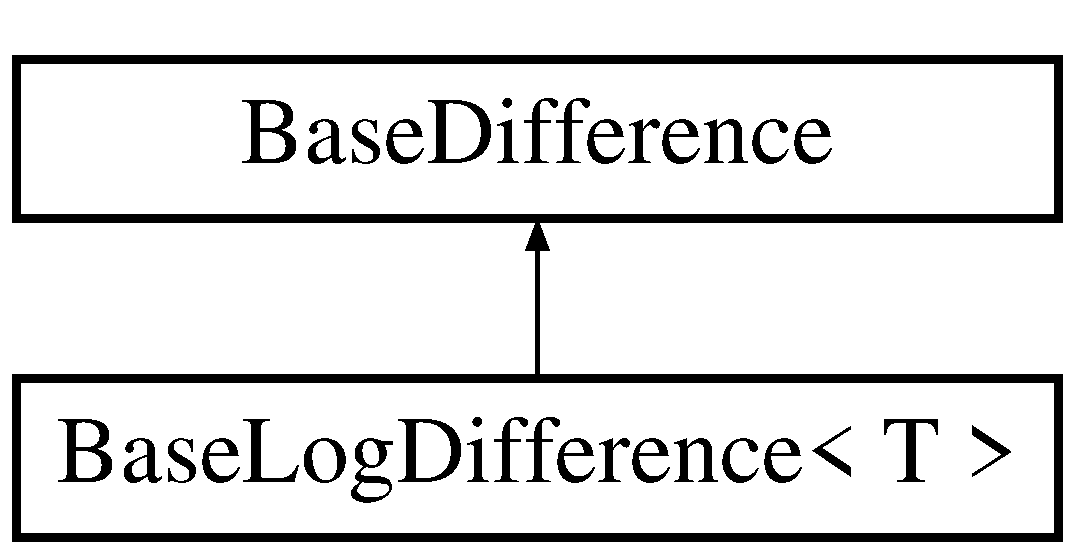
\includegraphics[height=2.000000cm]{classBaseDifference}
\end{center}
\end{figure}
\subsection*{Public Member Functions}
\begin{DoxyCompactItemize}
\item 
\hyperlink{classBaseDifference_ad9fe8c26c1ce15bc9e89bbfba57018af}{Base\+Difference} ()
\item 
void {\bfseries set\+Check} (bool check)\hypertarget{classBaseDifference_a2f942b77a94f991b25b5b7d610f1e827}{}\label{classBaseDifference_a2f942b77a94f991b25b5b7d610f1e827}

\item 
bool {\bfseries get\+Check} ()\hypertarget{classBaseDifference_a4fc53b0783ce154971468ae1e03bb1ec}{}\label{classBaseDifference_a4fc53b0783ce154971468ae1e03bb1ec}

\item 
void {\bfseries set\+Prop} (string prop)\hypertarget{classBaseDifference_a07199ac3c1cb1182caa73b2409608ea9}{}\label{classBaseDifference_a07199ac3c1cb1182caa73b2409608ea9}

\item 
string {\bfseries get\+Prop} ()\hypertarget{classBaseDifference_af8f73848d23d96034d2c326fbd258f2a}{}\label{classBaseDifference_af8f73848d23d96034d2c326fbd258f2a}

\item 
virtual void \hyperlink{classBaseDifference_ab369b45441dc65ae4346031872b70122}{visit\+To\+Assign} (\hyperlink{classVisitor}{Visitor} \&v, string to\+Assign)=0
\item 
virtual void \hyperlink{classBaseDifference_ab7a85a4a4ef9ef3a3e9abc97d3e19af4}{visit\+To\+Print} (\hyperlink{classVisitor}{Visitor} \&v)=0
\end{DoxyCompactItemize}
\subsection*{Protected Attributes}
\begin{DoxyCompactItemize}
\item 
bool {\bfseries check}\hypertarget{classBaseDifference_a28ad8522789fca062d1f14cf60ca34fa}{}\label{classBaseDifference_a28ad8522789fca062d1f14cf60ca34fa}

\item 
string {\bfseries prop}\hypertarget{classBaseDifference_ac476496c52f737394c5c4d42df4e3f9d}{}\label{classBaseDifference_ac476496c52f737394c5c4d42df4e3f9d}

\end{DoxyCompactItemize}


\subsection{Detailed Description}
Models a basic difference 

\subsection{Constructor \& Destructor Documentation}
\index{Base\+Difference@{Base\+Difference}!Base\+Difference@{Base\+Difference}}
\index{Base\+Difference@{Base\+Difference}!Base\+Difference@{Base\+Difference}}
\subsubsection[{\texorpdfstring{Base\+Difference()}{BaseDifference()}}]{\setlength{\rightskip}{0pt plus 5cm}Base\+Difference\+::\+Base\+Difference (
\begin{DoxyParamCaption}
{}
\end{DoxyParamCaption}
)\hspace{0.3cm}{\ttfamily [inline]}}\hypertarget{classBaseDifference_ad9fe8c26c1ce15bc9e89bbfba57018af}{}\label{classBaseDifference_ad9fe8c26c1ce15bc9e89bbfba57018af}
Default = no difference 

\subsection{Member Function Documentation}
\index{Base\+Difference@{Base\+Difference}!visit\+To\+Assign@{visit\+To\+Assign}}
\index{visit\+To\+Assign@{visit\+To\+Assign}!Base\+Difference@{Base\+Difference}}
\subsubsection[{\texorpdfstring{visit\+To\+Assign(\+Visitor \&v, string to\+Assign)=0}{visitToAssign(Visitor &v, string toAssign)=0}}]{\setlength{\rightskip}{0pt plus 5cm}virtual void Base\+Difference\+::visit\+To\+Assign (
\begin{DoxyParamCaption}
\item[{{\bf Visitor} \&}]{v, }
\item[{string}]{to\+Assign}
\end{DoxyParamCaption}
)\hspace{0.3cm}{\ttfamily [pure virtual]}}\hypertarget{classBaseDifference_ab369b45441dc65ae4346031872b70122}{}\label{classBaseDifference_ab369b45441dc65ae4346031872b70122}
Method used to visit the base difference and set his generic value


\begin{DoxyParams}{Parameters}
{\em v} & visitor used to visit the base difference \\
\hline
{\em to\+Assign} & value to assign, it\textquotesingle{}s a string and the specific implementation will know how to handle and cast it properly \\
\hline
\end{DoxyParams}


Implemented in \hyperlink{classBaseLogDifference_ad2174b64f0c611ea9398d49226f48f4f}{Base\+Log\+Difference$<$ T $>$}.

\index{Base\+Difference@{Base\+Difference}!visit\+To\+Print@{visit\+To\+Print}}
\index{visit\+To\+Print@{visit\+To\+Print}!Base\+Difference@{Base\+Difference}}
\subsubsection[{\texorpdfstring{visit\+To\+Print(\+Visitor \&v)=0}{visitToPrint(Visitor &v)=0}}]{\setlength{\rightskip}{0pt plus 5cm}virtual void Base\+Difference\+::visit\+To\+Print (
\begin{DoxyParamCaption}
\item[{{\bf Visitor} \&}]{v}
\end{DoxyParamCaption}
)\hspace{0.3cm}{\ttfamily [pure virtual]}}\hypertarget{classBaseDifference_ab7a85a4a4ef9ef3a3e9abc97d3e19af4}{}\label{classBaseDifference_ab7a85a4a4ef9ef3a3e9abc97d3e19af4}
Method used to visit the base difference and print his property


\begin{DoxyParams}{Parameters}
{\em v} & visitor used to print it. \\
\hline
\end{DoxyParams}


Implemented in \hyperlink{classBaseLogDifference_aedf247712392189dc236bd82e8fa8ea0}{Base\+Log\+Difference$<$ T $>$}.



The documentation for this class was generated from the following file\+:\begin{DoxyCompactItemize}
\item 
/home/doomdiskday/workspace2/main/src/model/\+H\+W/\+Basic/Base\+Difference.\+h\end{DoxyCompactItemize}

\hypertarget{classBaseInfo}{}\section{Base\+Info$<$ T $>$ Class Template Reference}
\label{classBaseInfo}\index{Base\+Info$<$ T $>$@{Base\+Info$<$ T $>$}}
Inheritance diagram for Base\+Info$<$ T $>$\+:\begin{figure}[H]
\begin{center}
\leavevmode
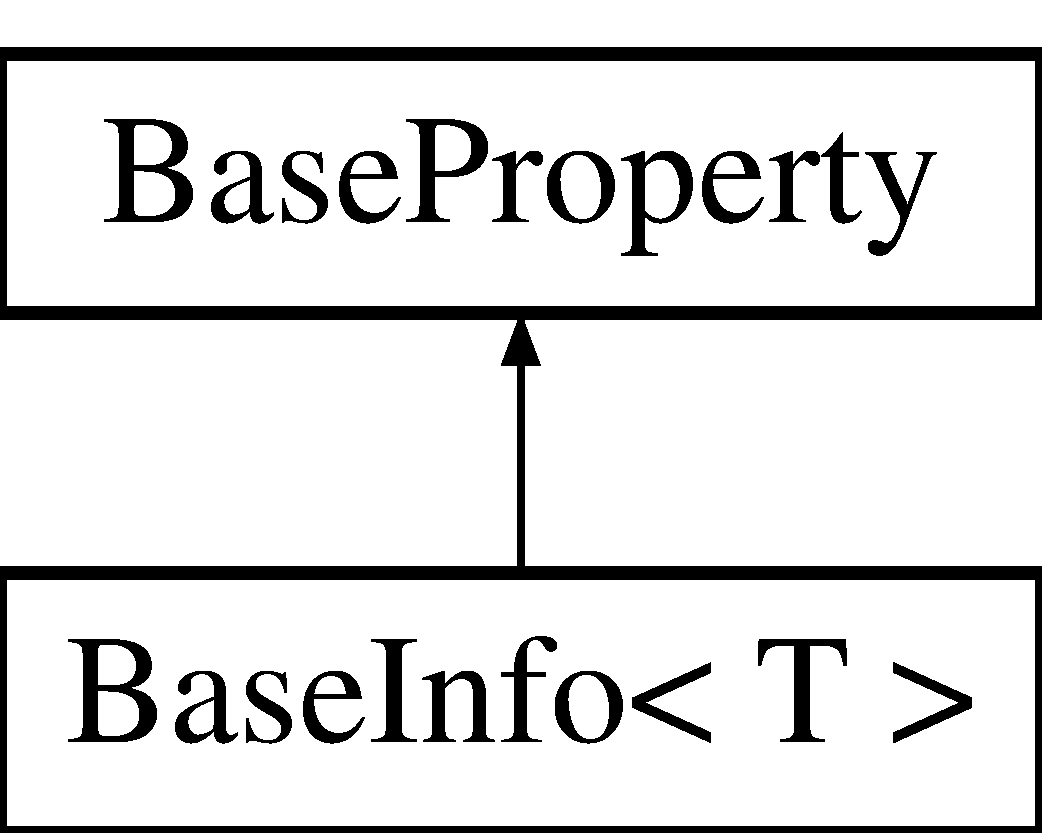
\includegraphics[height=2.000000cm]{classBaseInfo}
\end{center}
\end{figure}
\subsection*{Public Member Functions}
\begin{DoxyCompactItemize}
\item 
void {\bfseries set\+Value} (T value)\hypertarget{classBaseInfo_a09e8ede57d2eaad37b868ca2dafce74f}{}\label{classBaseInfo_a09e8ede57d2eaad37b868ca2dafce74f}

\item 
T {\bfseries get\+Value} ()\hypertarget{classBaseInfo_af3590382940cb865a5a8bb59d5d052af}{}\label{classBaseInfo_af3590382940cb865a5a8bb59d5d052af}

\item 
void \hyperlink{classBaseInfo_a84d4e0585478afa4fa067e7485a69159}{visit\+Value\+With\+Base\+Command} (\hyperlink{classVisitor}{Visitor} \&visitor, \hyperlink{classCommand}{Command} $\ast$cmd)
\item 
void \hyperlink{classBaseInfo_a903966b7c9bb3e206b72d7e167d0102a}{visit\+To\+Print} (\hyperlink{classVisitor}{Visitor} \&v)
\item 
void \hyperlink{classBaseInfo_aec2c01b1d1c5a1d8322e4e1c294872d5}{visit\+To\+Log} (\hyperlink{classVisitor}{Visitor} \&v, F\+I\+LE $\ast$log\+File)
\item 
void \hyperlink{classBaseInfo_aab20a2adc240dea5945e0c4340ade696}{visit\+To\+Assign} (\hyperlink{classVisitor}{Visitor} \&v, string to\+Assign)
\end{DoxyCompactItemize}


\subsection{Member Function Documentation}
\index{Base\+Info@{Base\+Info}!visit\+To\+Assign@{visit\+To\+Assign}}
\index{visit\+To\+Assign@{visit\+To\+Assign}!Base\+Info@{Base\+Info}}
\subsubsection[{\texorpdfstring{visit\+To\+Assign(\+Visitor \&v, string to\+Assign)}{visitToAssign(Visitor &v, string toAssign)}}]{\setlength{\rightskip}{0pt plus 5cm}template$<$class T$>$ void {\bf Base\+Info}$<$ T $>$\+::visit\+To\+Assign (
\begin{DoxyParamCaption}
\item[{{\bf Visitor} \&}]{v, }
\item[{string}]{to\+Assign}
\end{DoxyParamCaption}
)\hspace{0.3cm}{\ttfamily [inline]}, {\ttfamily [virtual]}}\hypertarget{classBaseInfo_aab20a2adc240dea5945e0c4340ade696}{}\label{classBaseInfo_aab20a2adc240dea5945e0c4340ade696}
Visit the object and assign his generic value.


\begin{DoxyParams}{Parameters}
{\em v} & the visitor used \\
\hline
{\em to\+Assign} & the value to assign (it\textquotesingle{}s everytime a string and the visitor will know how to cast it properly) \\
\hline
\end{DoxyParams}


Implements \hyperlink{classBaseProperty_a5213a052c34530a5f561149d7b48db60}{Base\+Property}.

\index{Base\+Info@{Base\+Info}!visit\+To\+Log@{visit\+To\+Log}}
\index{visit\+To\+Log@{visit\+To\+Log}!Base\+Info@{Base\+Info}}
\subsubsection[{\texorpdfstring{visit\+To\+Log(\+Visitor \&v, F\+I\+L\+E $\ast$log\+File)}{visitToLog(Visitor &v, FILE *logFile)}}]{\setlength{\rightskip}{0pt plus 5cm}template$<$class T$>$ void {\bf Base\+Info}$<$ T $>$\+::visit\+To\+Log (
\begin{DoxyParamCaption}
\item[{{\bf Visitor} \&}]{v, }
\item[{F\+I\+LE $\ast$}]{log\+File}
\end{DoxyParamCaption}
)\hspace{0.3cm}{\ttfamily [inline]}, {\ttfamily [virtual]}}\hypertarget{classBaseInfo_aec2c01b1d1c5a1d8322e4e1c294872d5}{}\label{classBaseInfo_aec2c01b1d1c5a1d8322e4e1c294872d5}
Visit the object and log it into a log file


\begin{DoxyParams}{Parameters}
{\em v} & the visitor used \\
\hline
{\em log\+File} & the log file \\
\hline
\end{DoxyParams}


Implements \hyperlink{classBaseProperty_a9e5f999d32dc4b0943948a70689565a1}{Base\+Property}.

\index{Base\+Info@{Base\+Info}!visit\+To\+Print@{visit\+To\+Print}}
\index{visit\+To\+Print@{visit\+To\+Print}!Base\+Info@{Base\+Info}}
\subsubsection[{\texorpdfstring{visit\+To\+Print(\+Visitor \&v)}{visitToPrint(Visitor &v)}}]{\setlength{\rightskip}{0pt plus 5cm}template$<$class T$>$ void {\bf Base\+Info}$<$ T $>$\+::visit\+To\+Print (
\begin{DoxyParamCaption}
\item[{{\bf Visitor} \&}]{v}
\end{DoxyParamCaption}
)\hspace{0.3cm}{\ttfamily [inline]}, {\ttfamily [virtual]}}\hypertarget{classBaseInfo_a903966b7c9bb3e206b72d7e167d0102a}{}\label{classBaseInfo_a903966b7c9bb3e206b72d7e167d0102a}
Visit the object and print his content


\begin{DoxyParams}{Parameters}
{\em v} & the visitor used to print \\
\hline
\end{DoxyParams}


Implements \hyperlink{classBaseProperty_a3c5334878537be377d3d50cc8b5091be}{Base\+Property}.

\index{Base\+Info@{Base\+Info}!visit\+Value\+With\+Base\+Command@{visit\+Value\+With\+Base\+Command}}
\index{visit\+Value\+With\+Base\+Command@{visit\+Value\+With\+Base\+Command}!Base\+Info@{Base\+Info}}
\subsubsection[{\texorpdfstring{visit\+Value\+With\+Base\+Command(\+Visitor \&visitor, Command $\ast$cmd)}{visitValueWithBaseCommand(Visitor &visitor, Command *cmd)}}]{\setlength{\rightskip}{0pt plus 5cm}template$<$class T$>$ void {\bf Base\+Info}$<$ T $>$\+::visit\+Value\+With\+Base\+Command (
\begin{DoxyParamCaption}
\item[{{\bf Visitor} \&}]{v, }
\item[{{\bf Command} $\ast$}]{cmd}
\end{DoxyParamCaption}
)\hspace{0.3cm}{\ttfamily [inline]}, {\ttfamily [virtual]}}\hypertarget{classBaseInfo_a84d4e0585478afa4fa067e7485a69159}{}\label{classBaseInfo_a84d4e0585478afa4fa067e7485a69159}
Visit the object and set his generic value with a command


\begin{DoxyParams}{Parameters}
{\em v} & the visitor used to set the value \\
\hline
{\em cmd} & the command used to set the value \\
\hline
\end{DoxyParams}


Implements \hyperlink{classBaseProperty_a83a5d6b8ebee03e73e11a7a57df56df3}{Base\+Property}.



The documentation for this class was generated from the following file\+:\begin{DoxyCompactItemize}
\item 
/home/doomdiskday/workspace2/main/src/model/\+H\+W/\+Basic/Base\+Info.\+h\end{DoxyCompactItemize}

\hypertarget{classBaseInfoComparator}{}\section{Base\+Info\+Comparator Class Reference}
\label{classBaseInfoComparator}\index{Base\+Info\+Comparator@{Base\+Info\+Comparator}}


{\ttfamily \#include $<$Base\+Info\+Comparator.\+h$>$}

\subsection*{Public Member Functions}
\begin{DoxyCompactItemize}
\item 
bool {\bfseries compare} (\hyperlink{classBaseProperty}{Base\+Property} $\ast$orig, \hyperlink{classBaseProperty}{Base\+Property} $\ast$to\+Check, \hyperlink{classBaseDifference}{Base\+Difference} $\ast$log)\hypertarget{classBaseInfoComparator_ab9451e03f463dc4bcaa995c64916a1db}{}\label{classBaseInfoComparator_ab9451e03f463dc4bcaa995c64916a1db}

\item 
bool {\bfseries visit\+To\+Compare} (\hyperlink{classBaseInfo}{Base\+Info}$<$ int $>$ $\ast$orig, \hyperlink{classBaseInfo}{Base\+Info}$<$ int $>$ $\ast$to\+Check, \hyperlink{classBaseDifference}{Base\+Difference} $\ast$log)\hypertarget{classBaseInfoComparator_a5e80cb49f73f2a2bb6cdeac8e09e6dc3}{}\label{classBaseInfoComparator_a5e80cb49f73f2a2bb6cdeac8e09e6dc3}

\item 
bool {\bfseries visit\+To\+Compare} (\hyperlink{classBaseInfo}{Base\+Info}$<$ string $>$ $\ast$orig, \hyperlink{classBaseInfo}{Base\+Info}$<$ string $>$ $\ast$to\+Check, \hyperlink{classBaseDifference}{Base\+Difference} $\ast$log)\hypertarget{classBaseInfoComparator_a09e5add363c7e953fa09b40eae7843ee}{}\label{classBaseInfoComparator_a09e5add363c7e953fa09b40eae7843ee}

\end{DoxyCompactItemize}


\subsection{Detailed Description}
This comparator compare two different Base\+Properties and set a log difference to the correct value. Contains two different implementations (int and string) for the comparisons 

The documentation for this class was generated from the following file\+:\begin{DoxyCompactItemize}
\item 
/home/doomdiskday/workspace2/main/src/utils/Base\+Info\+Comparator.\+h\end{DoxyCompactItemize}

\hypertarget{classBaseInfoVisitor}{}\section{Base\+Info\+Visitor Class Reference}
\label{classBaseInfoVisitor}\index{Base\+Info\+Visitor@{Base\+Info\+Visitor}}


{\ttfamily \#include $<$Base\+Info\+Visitor.\+h$>$}

Inheritance diagram for Base\+Info\+Visitor\+:\begin{figure}[H]
\begin{center}
\leavevmode
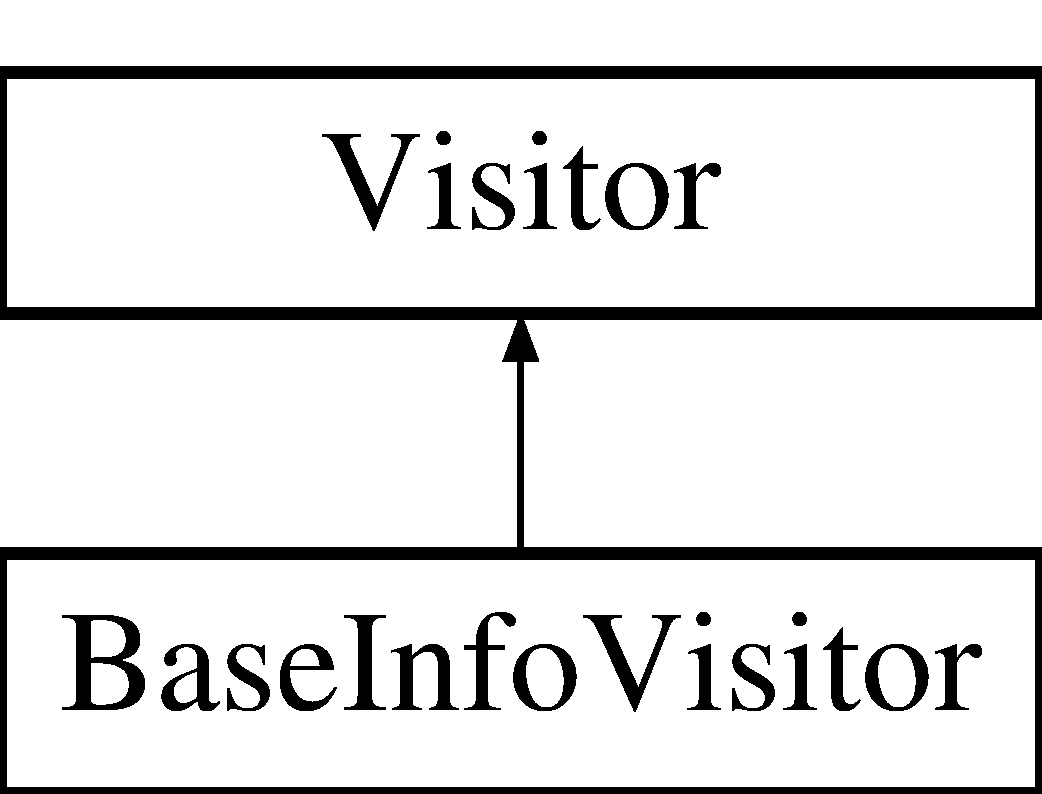
\includegraphics[height=2.000000cm]{classBaseInfoVisitor}
\end{center}
\end{figure}
\subsection*{Public Member Functions}
\begin{DoxyCompactItemize}
\item 
void \hyperlink{classBaseInfoVisitor_a96013581736191e0c186746f061b6d2e}{visit\+Base\+Info\+With\+Command} (int \&v, \hyperlink{classCommand}{Command} $\ast$cmd)
\item 
void \hyperlink{classBaseInfoVisitor_a8615d145a52433f981a147642038fe91}{visit\+Base\+Info\+With\+Command} (string \&v, \hyperlink{classCommand}{Command} $\ast$cmd)
\item 
void \hyperlink{classBaseInfoVisitor_a395234ebebdfbaf4f7e155bfc0a5aa5d}{visit\+Base\+Info\+To\+Print} (int v, string property)
\item 
void \hyperlink{classBaseInfoVisitor_a5be08c690d21e5c1d9257efdf0a75ca4}{visit\+Base\+Info\+To\+Print} (string v, string property)
\item 
void \hyperlink{classBaseInfoVisitor_adf0f9a3ad34d26595ee2cb78cc370a65}{visit\+Base\+Info\+To\+Log} (int v, string property, F\+I\+LE $\ast$log\+File)
\item 
void \hyperlink{classBaseInfoVisitor_a8590d40b5c1c277dee482518ad31c494}{visit\+Base\+Info\+To\+Log} (string v, string property, F\+I\+LE $\ast$log\+File)
\item 
void \hyperlink{classBaseInfoVisitor_a56c3bb5a441e77566e62881e5a82b9d8}{visit\+Base\+Info\+With\+Value} (int \&v, string to\+Assign)
\item 
void \hyperlink{classBaseInfoVisitor_adc07ce4d4919fccad038d90c9c820178}{visit\+Base\+Info\+With\+Value} (string \&v, string to\+Assign)
\item 
void \hyperlink{classBaseInfoVisitor_ad0c9667e9004fd1494f79b09947b0620}{visit\+Log\+To\+Print} (bool check, string prop, string value)
\item 
void \hyperlink{classBaseInfoVisitor_a326f9be710640548f76a08253422318a}{visit\+Log\+To\+Print} (bool check, string prop, int value)
\item 
void {\bfseries visit\+And\+Set\+Base\+Log\+Visitor} (string \&to\+Assign, string value)\hypertarget{classBaseInfoVisitor_a4782e630fd239dca702d5572c483ddf7}{}\label{classBaseInfoVisitor_a4782e630fd239dca702d5572c483ddf7}

\end{DoxyCompactItemize}


\subsection{Detailed Description}
This class model a visitor able to visit properties and log differences and manage them 

\subsection{Member Function Documentation}
\index{Base\+Info\+Visitor@{Base\+Info\+Visitor}!visit\+Base\+Info\+To\+Log@{visit\+Base\+Info\+To\+Log}}
\index{visit\+Base\+Info\+To\+Log@{visit\+Base\+Info\+To\+Log}!Base\+Info\+Visitor@{Base\+Info\+Visitor}}
\subsubsection[{\texorpdfstring{visit\+Base\+Info\+To\+Log(int v, string property, F\+I\+L\+E $\ast$log\+File)}{visitBaseInfoToLog(int v, string property, FILE *logFile)}}]{\setlength{\rightskip}{0pt plus 5cm}void Base\+Info\+Visitor\+::visit\+Base\+Info\+To\+Log (
\begin{DoxyParamCaption}
\item[{int}]{v, }
\item[{string}]{property, }
\item[{F\+I\+LE $\ast$}]{log\+File}
\end{DoxyParamCaption}
)\hspace{0.3cm}{\ttfamily [inline]}, {\ttfamily [virtual]}}\hypertarget{classBaseInfoVisitor_adf0f9a3ad34d26595ee2cb78cc370a65}{}\label{classBaseInfoVisitor_adf0f9a3ad34d26595ee2cb78cc370a65}
Method used to visit a baseinfo and log his value and his property


\begin{DoxyParams}{Parameters}
{\em v} & the int value to log \\
\hline
{\em property} & the property to log \\
\hline
{\em log\+File} & the log file to populate. \\
\hline
\end{DoxyParams}


Implements \hyperlink{classVisitor_addcf4dbedba4a2ba739d0fdef144eb6d}{Visitor}.

\index{Base\+Info\+Visitor@{Base\+Info\+Visitor}!visit\+Base\+Info\+To\+Log@{visit\+Base\+Info\+To\+Log}}
\index{visit\+Base\+Info\+To\+Log@{visit\+Base\+Info\+To\+Log}!Base\+Info\+Visitor@{Base\+Info\+Visitor}}
\subsubsection[{\texorpdfstring{visit\+Base\+Info\+To\+Log(string v, string property, F\+I\+L\+E $\ast$log\+File)}{visitBaseInfoToLog(string v, string property, FILE *logFile)}}]{\setlength{\rightskip}{0pt plus 5cm}void Base\+Info\+Visitor\+::visit\+Base\+Info\+To\+Log (
\begin{DoxyParamCaption}
\item[{string}]{v, }
\item[{string}]{property, }
\item[{F\+I\+LE $\ast$}]{log\+File}
\end{DoxyParamCaption}
)\hspace{0.3cm}{\ttfamily [inline]}, {\ttfamily [virtual]}}\hypertarget{classBaseInfoVisitor_a8590d40b5c1c277dee482518ad31c494}{}\label{classBaseInfoVisitor_a8590d40b5c1c277dee482518ad31c494}
Method used to visit a baseinfo and log his value and his property


\begin{DoxyParams}{Parameters}
{\em v} & the string value to log \\
\hline
{\em property} & the property to log \\
\hline
{\em log\+File} & the log file to populate. \\
\hline
\end{DoxyParams}


Implements \hyperlink{classVisitor_a591ed3a6edd9b31a8a1b2847c5a22e29}{Visitor}.

\index{Base\+Info\+Visitor@{Base\+Info\+Visitor}!visit\+Base\+Info\+To\+Print@{visit\+Base\+Info\+To\+Print}}
\index{visit\+Base\+Info\+To\+Print@{visit\+Base\+Info\+To\+Print}!Base\+Info\+Visitor@{Base\+Info\+Visitor}}
\subsubsection[{\texorpdfstring{visit\+Base\+Info\+To\+Print(int v, string property)}{visitBaseInfoToPrint(int v, string property)}}]{\setlength{\rightskip}{0pt plus 5cm}void Base\+Info\+Visitor\+::visit\+Base\+Info\+To\+Print (
\begin{DoxyParamCaption}
\item[{int}]{v, }
\item[{string}]{property}
\end{DoxyParamCaption}
)\hspace{0.3cm}{\ttfamily [inline]}, {\ttfamily [virtual]}}\hypertarget{classBaseInfoVisitor_a395234ebebdfbaf4f7e155bfc0a5aa5d}{}\label{classBaseInfoVisitor_a395234ebebdfbaf4f7e155bfc0a5aa5d}
Method used to visit a baseinfo and print his value and his property


\begin{DoxyParams}{Parameters}
{\em v} & the int value to print \\
\hline
{\em property} & the property to print \\
\hline
\end{DoxyParams}


Implements \hyperlink{classVisitor_a3d6f39af42e955dcd56d1d928f6edfe2}{Visitor}.

\index{Base\+Info\+Visitor@{Base\+Info\+Visitor}!visit\+Base\+Info\+To\+Print@{visit\+Base\+Info\+To\+Print}}
\index{visit\+Base\+Info\+To\+Print@{visit\+Base\+Info\+To\+Print}!Base\+Info\+Visitor@{Base\+Info\+Visitor}}
\subsubsection[{\texorpdfstring{visit\+Base\+Info\+To\+Print(string v, string property)}{visitBaseInfoToPrint(string v, string property)}}]{\setlength{\rightskip}{0pt plus 5cm}void Base\+Info\+Visitor\+::visit\+Base\+Info\+To\+Print (
\begin{DoxyParamCaption}
\item[{string}]{v, }
\item[{string}]{property}
\end{DoxyParamCaption}
)\hspace{0.3cm}{\ttfamily [inline]}, {\ttfamily [virtual]}}\hypertarget{classBaseInfoVisitor_a5be08c690d21e5c1d9257efdf0a75ca4}{}\label{classBaseInfoVisitor_a5be08c690d21e5c1d9257efdf0a75ca4}
Method used to visit a baseinfo and print his value and his property


\begin{DoxyParams}{Parameters}
{\em v} & the string value to print \\
\hline
{\em property} & the property to print \\
\hline
\end{DoxyParams}


Implements \hyperlink{classVisitor_a9f87fbabd6b8cd4d5456d81faff2c31a}{Visitor}.

\index{Base\+Info\+Visitor@{Base\+Info\+Visitor}!visit\+Base\+Info\+With\+Command@{visit\+Base\+Info\+With\+Command}}
\index{visit\+Base\+Info\+With\+Command@{visit\+Base\+Info\+With\+Command}!Base\+Info\+Visitor@{Base\+Info\+Visitor}}
\subsubsection[{\texorpdfstring{visit\+Base\+Info\+With\+Command(int \&v, Command $\ast$cmd)}{visitBaseInfoWithCommand(int &v, Command *cmd)}}]{\setlength{\rightskip}{0pt plus 5cm}void Base\+Info\+Visitor\+::visit\+Base\+Info\+With\+Command (
\begin{DoxyParamCaption}
\item[{int \&}]{v, }
\item[{{\bf Command} $\ast$}]{cmd}
\end{DoxyParamCaption}
)\hspace{0.3cm}{\ttfamily [inline]}, {\ttfamily [virtual]}}\hypertarget{classBaseInfoVisitor_a96013581736191e0c186746f061b6d2e}{}\label{classBaseInfoVisitor_a96013581736191e0c186746f061b6d2e}
Method used to visit a baseinfo and set his value to an information retrieved by a command passed by param


\begin{DoxyParams}{Parameters}
{\em v} & the int value to set \\
\hline
{\em cmd} & the command used \\
\hline
\end{DoxyParams}


Implements \hyperlink{classVisitor_aa290c4e12905eb700f631b83ce77deea}{Visitor}.

\index{Base\+Info\+Visitor@{Base\+Info\+Visitor}!visit\+Base\+Info\+With\+Command@{visit\+Base\+Info\+With\+Command}}
\index{visit\+Base\+Info\+With\+Command@{visit\+Base\+Info\+With\+Command}!Base\+Info\+Visitor@{Base\+Info\+Visitor}}
\subsubsection[{\texorpdfstring{visit\+Base\+Info\+With\+Command(string \&v, Command $\ast$cmd)}{visitBaseInfoWithCommand(string &v, Command *cmd)}}]{\setlength{\rightskip}{0pt plus 5cm}void Base\+Info\+Visitor\+::visit\+Base\+Info\+With\+Command (
\begin{DoxyParamCaption}
\item[{string \&}]{v, }
\item[{{\bf Command} $\ast$}]{cmd}
\end{DoxyParamCaption}
)\hspace{0.3cm}{\ttfamily [inline]}, {\ttfamily [virtual]}}\hypertarget{classBaseInfoVisitor_a8615d145a52433f981a147642038fe91}{}\label{classBaseInfoVisitor_a8615d145a52433f981a147642038fe91}
Method used to visit a baseinfo and set his value to an information retrieved by a command passed by param


\begin{DoxyParams}{Parameters}
{\em v} & the string value to set \\
\hline
{\em cmd} & the command used \\
\hline
\end{DoxyParams}


Implements \hyperlink{classVisitor_aa6045f028cc91712ab5cca38e1461d39}{Visitor}.

\index{Base\+Info\+Visitor@{Base\+Info\+Visitor}!visit\+Base\+Info\+With\+Value@{visit\+Base\+Info\+With\+Value}}
\index{visit\+Base\+Info\+With\+Value@{visit\+Base\+Info\+With\+Value}!Base\+Info\+Visitor@{Base\+Info\+Visitor}}
\subsubsection[{\texorpdfstring{visit\+Base\+Info\+With\+Value(int \&v, string to\+Assign)}{visitBaseInfoWithValue(int &v, string toAssign)}}]{\setlength{\rightskip}{0pt plus 5cm}void Base\+Info\+Visitor\+::visit\+Base\+Info\+With\+Value (
\begin{DoxyParamCaption}
\item[{int \&}]{v, }
\item[{string}]{to\+Assign}
\end{DoxyParamCaption}
)\hspace{0.3cm}{\ttfamily [inline]}, {\ttfamily [virtual]}}\hypertarget{classBaseInfoVisitor_a56c3bb5a441e77566e62881e5a82b9d8}{}\label{classBaseInfoVisitor_a56c3bb5a441e77566e62881e5a82b9d8}
Method used to visit a baseinfo and set his value.


\begin{DoxyParams}{Parameters}
{\em v} & the int value to set \\
\hline
{\em property} & the property to set \\
\hline
\end{DoxyParams}


Implements \hyperlink{classVisitor_a766dd43ac0c15f92b15a5b0fb90deca9}{Visitor}.

\index{Base\+Info\+Visitor@{Base\+Info\+Visitor}!visit\+Base\+Info\+With\+Value@{visit\+Base\+Info\+With\+Value}}
\index{visit\+Base\+Info\+With\+Value@{visit\+Base\+Info\+With\+Value}!Base\+Info\+Visitor@{Base\+Info\+Visitor}}
\subsubsection[{\texorpdfstring{visit\+Base\+Info\+With\+Value(string \&v, string to\+Assign)}{visitBaseInfoWithValue(string &v, string toAssign)}}]{\setlength{\rightskip}{0pt plus 5cm}void Base\+Info\+Visitor\+::visit\+Base\+Info\+With\+Value (
\begin{DoxyParamCaption}
\item[{string \&}]{v, }
\item[{string}]{to\+Assign}
\end{DoxyParamCaption}
)\hspace{0.3cm}{\ttfamily [inline]}, {\ttfamily [virtual]}}\hypertarget{classBaseInfoVisitor_adc07ce4d4919fccad038d90c9c820178}{}\label{classBaseInfoVisitor_adc07ce4d4919fccad038d90c9c820178}
Method used to visit a baseinfo and set his value.


\begin{DoxyParams}{Parameters}
{\em v} & the string value to set \\
\hline
{\em property} & the property to set \\
\hline
\end{DoxyParams}


Implements \hyperlink{classVisitor_afb85cf66df37046633ef80f085c8c4fe}{Visitor}.

\index{Base\+Info\+Visitor@{Base\+Info\+Visitor}!visit\+Log\+To\+Print@{visit\+Log\+To\+Print}}
\index{visit\+Log\+To\+Print@{visit\+Log\+To\+Print}!Base\+Info\+Visitor@{Base\+Info\+Visitor}}
\subsubsection[{\texorpdfstring{visit\+Log\+To\+Print(bool check, string prop, string value)}{visitLogToPrint(bool check, string prop, string value)}}]{\setlength{\rightskip}{0pt plus 5cm}void Base\+Info\+Visitor\+::visit\+Log\+To\+Print (
\begin{DoxyParamCaption}
\item[{bool}]{check, }
\item[{string}]{prop, }
\item[{string}]{value}
\end{DoxyParamCaption}
)\hspace{0.3cm}{\ttfamily [inline]}, {\ttfamily [virtual]}}\hypertarget{classBaseInfoVisitor_ad0c9667e9004fd1494f79b09947b0620}{}\label{classBaseInfoVisitor_ad0c9667e9004fd1494f79b09947b0620}
Method used to visit a log file and populate it


\begin{DoxyParams}{Parameters}
{\em check} & the check value \\
\hline
{\em prop} & the property checked \\
\hline
{\em value} & the value checked \\
\hline
\end{DoxyParams}


Implements \hyperlink{classVisitor_a3e8e80f88fd9513a971f4db4cde00ef7}{Visitor}.

\index{Base\+Info\+Visitor@{Base\+Info\+Visitor}!visit\+Log\+To\+Print@{visit\+Log\+To\+Print}}
\index{visit\+Log\+To\+Print@{visit\+Log\+To\+Print}!Base\+Info\+Visitor@{Base\+Info\+Visitor}}
\subsubsection[{\texorpdfstring{visit\+Log\+To\+Print(bool check, string prop, int value)}{visitLogToPrint(bool check, string prop, int value)}}]{\setlength{\rightskip}{0pt plus 5cm}void Base\+Info\+Visitor\+::visit\+Log\+To\+Print (
\begin{DoxyParamCaption}
\item[{bool}]{check, }
\item[{string}]{prop, }
\item[{int}]{value}
\end{DoxyParamCaption}
)\hspace{0.3cm}{\ttfamily [inline]}, {\ttfamily [virtual]}}\hypertarget{classBaseInfoVisitor_a326f9be710640548f76a08253422318a}{}\label{classBaseInfoVisitor_a326f9be710640548f76a08253422318a}
Method used to visit a log file and populate it


\begin{DoxyParams}{Parameters}
{\em check} & the check value \\
\hline
{\em prop} & the property checked \\
\hline
{\em value} & the value checked \\
\hline
\end{DoxyParams}


Implements \hyperlink{classVisitor_ac889258497b1a2c2d673de0ceb3b227b}{Visitor}.



The documentation for this class was generated from the following file\+:\begin{DoxyCompactItemize}
\item 
/home/doomdiskday/workspace2/main/src/model/\+H\+W/\+Visitors/Base\+Info\+Visitor.\+h\end{DoxyCompactItemize}

\hypertarget{classBaseLogDifference}{}\section{Base\+Log\+Difference$<$ T $>$ Class Template Reference}
\label{classBaseLogDifference}\index{Base\+Log\+Difference$<$ T $>$@{Base\+Log\+Difference$<$ T $>$}}


{\ttfamily \#include $<$Base\+Log\+Difference.\+h$>$}

Inheritance diagram for Base\+Log\+Difference$<$ T $>$\+:\begin{figure}[H]
\begin{center}
\leavevmode
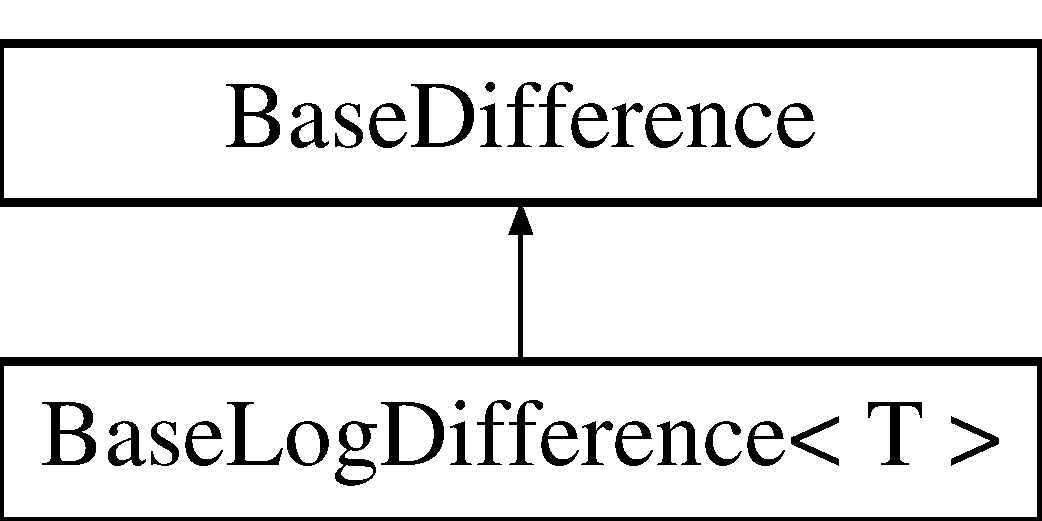
\includegraphics[height=2.000000cm]{classBaseLogDifference}
\end{center}
\end{figure}
\subsection*{Public Member Functions}
\begin{DoxyCompactItemize}
\item 
void {\bfseries set\+Value} (T value)\hypertarget{classBaseLogDifference_acaaeeaab163080f9ec47074a8db4fa3d}{}\label{classBaseLogDifference_acaaeeaab163080f9ec47074a8db4fa3d}

\item 
T {\bfseries get\+Value} ()\hypertarget{classBaseLogDifference_a1771f91aacb9e5b12b5d38de64285dc5}{}\label{classBaseLogDifference_a1771f91aacb9e5b12b5d38de64285dc5}

\item 
void \hyperlink{classBaseLogDifference_ad2174b64f0c611ea9398d49226f48f4f}{visit\+To\+Assign} (\hyperlink{classVisitor}{Visitor} \&v, string to\+Assign)
\item 
void \hyperlink{classBaseLogDifference_aedf247712392189dc236bd82e8fa8ea0}{visit\+To\+Print} (\hyperlink{classVisitor}{Visitor} \&v)
\end{DoxyCompactItemize}
\subsection*{Additional Inherited Members}


\subsection{Detailed Description}
\subsubsection*{template$<$class T$>$\\*
class Base\+Log\+Difference$<$ T $>$}

This template class rappresents a generic \hyperlink{classBaseLogDifference}{Base\+Log\+Difference} used to find difference during the checking phase. 

\subsection{Member Function Documentation}
\index{Base\+Log\+Difference@{Base\+Log\+Difference}!visit\+To\+Assign@{visit\+To\+Assign}}
\index{visit\+To\+Assign@{visit\+To\+Assign}!Base\+Log\+Difference@{Base\+Log\+Difference}}
\subsubsection[{\texorpdfstring{visit\+To\+Assign(\+Visitor \&v, string to\+Assign)}{visitToAssign(Visitor &v, string toAssign)}}]{\setlength{\rightskip}{0pt plus 5cm}template$<$class T $>$ void {\bf Base\+Log\+Difference}$<$ T $>$\+::visit\+To\+Assign (
\begin{DoxyParamCaption}
\item[{{\bf Visitor} \&}]{v, }
\item[{string}]{to\+Assign}
\end{DoxyParamCaption}
)\hspace{0.3cm}{\ttfamily [inline]}, {\ttfamily [virtual]}}\hypertarget{classBaseLogDifference_ad2174b64f0c611ea9398d49226f48f4f}{}\label{classBaseLogDifference_ad2174b64f0c611ea9398d49226f48f4f}
Method used to assign the T value by a visitor.


\begin{DoxyParams}{Parameters}
{\em v} & the visitor used \\
\hline
{\em to\+Assign} & the value to assign. it\textquotesingle{}s a string and the visitor will know how to cast it. \\
\hline
\end{DoxyParams}


Implements \hyperlink{classBaseDifference_ab369b45441dc65ae4346031872b70122}{Base\+Difference}.

\index{Base\+Log\+Difference@{Base\+Log\+Difference}!visit\+To\+Print@{visit\+To\+Print}}
\index{visit\+To\+Print@{visit\+To\+Print}!Base\+Log\+Difference@{Base\+Log\+Difference}}
\subsubsection[{\texorpdfstring{visit\+To\+Print(\+Visitor \&v)}{visitToPrint(Visitor &v)}}]{\setlength{\rightskip}{0pt plus 5cm}template$<$class T $>$ void {\bf Base\+Log\+Difference}$<$ T $>$\+::visit\+To\+Print (
\begin{DoxyParamCaption}
\item[{{\bf Visitor} \&}]{v}
\end{DoxyParamCaption}
)\hspace{0.3cm}{\ttfamily [inline]}, {\ttfamily [virtual]}}\hypertarget{classBaseLogDifference_aedf247712392189dc236bd82e8fa8ea0}{}\label{classBaseLogDifference_aedf247712392189dc236bd82e8fa8ea0}
Method used to print the generic value.


\begin{DoxyParams}{Parameters}
{\em v} & visitor used to print. \\
\hline
\end{DoxyParams}


Implements \hyperlink{classBaseDifference_ab7a85a4a4ef9ef3a3e9abc97d3e19af4}{Base\+Difference}.



The documentation for this class was generated from the following file\+:\begin{DoxyCompactItemize}
\item 
/home/doomdiskday/workspace2/main/src/model/\+H\+W/\+Basic/Base\+Log\+Difference.\+h\end{DoxyCompactItemize}

\hypertarget{classBaseProperty}{}\section{Base\+Property Class Reference}
\label{classBaseProperty}\index{Base\+Property@{Base\+Property}}


{\ttfamily \#include $<$Base\+Property.\+h$>$}

Inheritance diagram for Base\+Property\+:\begin{figure}[H]
\begin{center}
\leavevmode
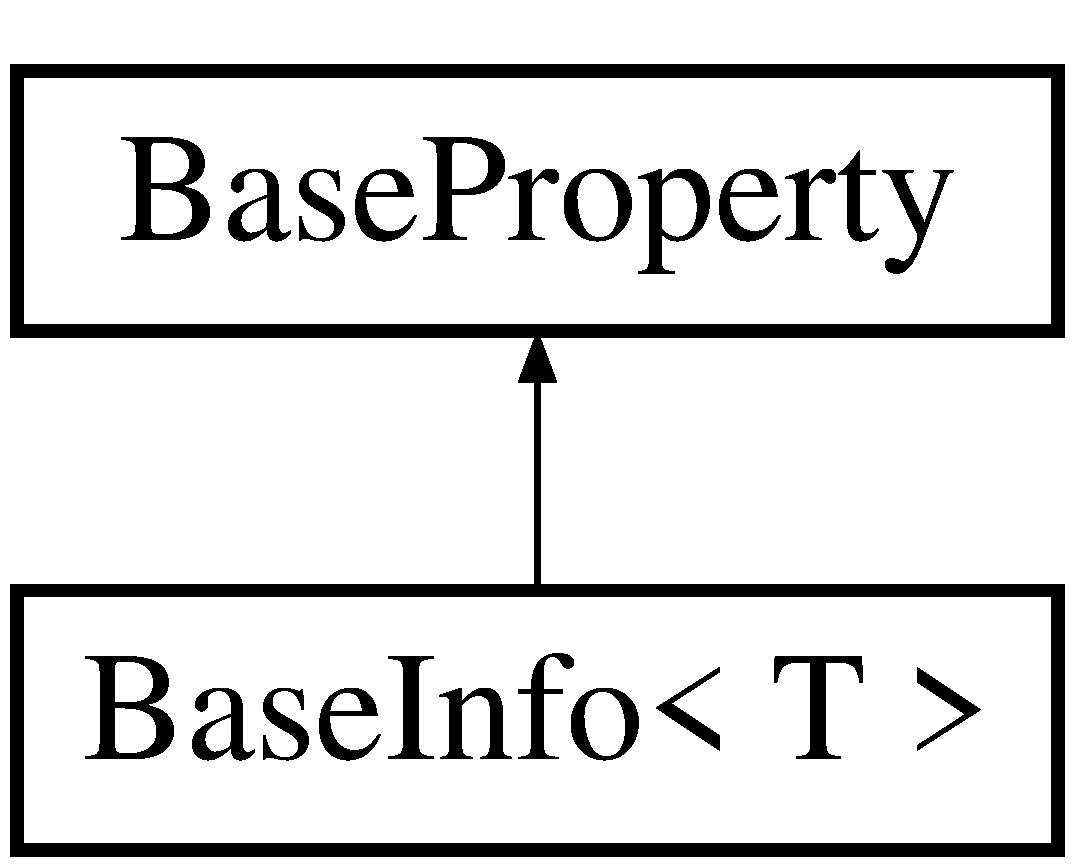
\includegraphics[height=2.000000cm]{classBaseProperty}
\end{center}
\end{figure}
\subsection*{Public Member Functions}
\begin{DoxyCompactItemize}
\item 
void {\bfseries set\+Property} (string property)\hypertarget{classBaseProperty_add91584f9f27a6f0f6d723042403445a}{}\label{classBaseProperty_add91584f9f27a6f0f6d723042403445a}

\item 
string {\bfseries get\+Property} ()\hypertarget{classBaseProperty_a403ce39c3c637bdc45078c9e7e52e2b3}{}\label{classBaseProperty_a403ce39c3c637bdc45078c9e7e52e2b3}

\item 
virtual void \hyperlink{classBaseProperty_a83a5d6b8ebee03e73e11a7a57df56df3}{visit\+Value\+With\+Base\+Command} (\hyperlink{classVisitor}{Visitor} \&v, \hyperlink{classCommand}{Command} $\ast$cmd)=0
\item 
virtual void \hyperlink{classBaseProperty_a3c5334878537be377d3d50cc8b5091be}{visit\+To\+Print} (\hyperlink{classVisitor}{Visitor} \&v)=0
\item 
virtual void \hyperlink{classBaseProperty_a9e5f999d32dc4b0943948a70689565a1}{visit\+To\+Log} (\hyperlink{classVisitor}{Visitor} \&v, F\+I\+LE $\ast$log\+File)=0
\item 
virtual void \hyperlink{classBaseProperty_a5213a052c34530a5f561149d7b48db60}{visit\+To\+Assign} (\hyperlink{classVisitor}{Visitor} \&v, string to\+Assign)=0
\end{DoxyCompactItemize}


\subsection{Detailed Description}
This class models a base property, it\textquotesingle{}s composed by a string only that rappresents the property name and is extended by  that model the final property composed by the value too 

\subsection{Member Function Documentation}
\index{Base\+Property@{Base\+Property}!visit\+To\+Assign@{visit\+To\+Assign}}
\index{visit\+To\+Assign@{visit\+To\+Assign}!Base\+Property@{Base\+Property}}
\subsubsection[{\texorpdfstring{visit\+To\+Assign(\+Visitor \&v, string to\+Assign)=0}{visitToAssign(Visitor &v, string toAssign)=0}}]{\setlength{\rightskip}{0pt plus 5cm}virtual void Base\+Property\+::visit\+To\+Assign (
\begin{DoxyParamCaption}
\item[{{\bf Visitor} \&}]{v, }
\item[{string}]{to\+Assign}
\end{DoxyParamCaption}
)\hspace{0.3cm}{\ttfamily [pure virtual]}}\hypertarget{classBaseProperty_a5213a052c34530a5f561149d7b48db60}{}\label{classBaseProperty_a5213a052c34530a5f561149d7b48db60}
Visit the object and assign his generic value.


\begin{DoxyParams}{Parameters}
{\em v} & the visitor used \\
\hline
{\em to\+Assign} & the value to assign (it\textquotesingle{}s everytime a string and the visitor will know how to cast it properly) \\
\hline
\end{DoxyParams}


Implemented in \hyperlink{classBaseInfo_aab20a2adc240dea5945e0c4340ade696}{Base\+Info$<$ T $>$}.

\index{Base\+Property@{Base\+Property}!visit\+To\+Log@{visit\+To\+Log}}
\index{visit\+To\+Log@{visit\+To\+Log}!Base\+Property@{Base\+Property}}
\subsubsection[{\texorpdfstring{visit\+To\+Log(\+Visitor \&v, F\+I\+L\+E $\ast$log\+File)=0}{visitToLog(Visitor &v, FILE *logFile)=0}}]{\setlength{\rightskip}{0pt plus 5cm}virtual void Base\+Property\+::visit\+To\+Log (
\begin{DoxyParamCaption}
\item[{{\bf Visitor} \&}]{v, }
\item[{F\+I\+LE $\ast$}]{log\+File}
\end{DoxyParamCaption}
)\hspace{0.3cm}{\ttfamily [pure virtual]}}\hypertarget{classBaseProperty_a9e5f999d32dc4b0943948a70689565a1}{}\label{classBaseProperty_a9e5f999d32dc4b0943948a70689565a1}
Visit the object and log it into a log file


\begin{DoxyParams}{Parameters}
{\em v} & the visitor used \\
\hline
{\em log\+File} & the log file \\
\hline
\end{DoxyParams}


Implemented in \hyperlink{classBaseInfo_aec2c01b1d1c5a1d8322e4e1c294872d5}{Base\+Info$<$ T $>$}.

\index{Base\+Property@{Base\+Property}!visit\+To\+Print@{visit\+To\+Print}}
\index{visit\+To\+Print@{visit\+To\+Print}!Base\+Property@{Base\+Property}}
\subsubsection[{\texorpdfstring{visit\+To\+Print(\+Visitor \&v)=0}{visitToPrint(Visitor &v)=0}}]{\setlength{\rightskip}{0pt plus 5cm}virtual void Base\+Property\+::visit\+To\+Print (
\begin{DoxyParamCaption}
\item[{{\bf Visitor} \&}]{v}
\end{DoxyParamCaption}
)\hspace{0.3cm}{\ttfamily [pure virtual]}}\hypertarget{classBaseProperty_a3c5334878537be377d3d50cc8b5091be}{}\label{classBaseProperty_a3c5334878537be377d3d50cc8b5091be}
Visit the object and print his content


\begin{DoxyParams}{Parameters}
{\em v} & the visitor used to print \\
\hline
\end{DoxyParams}


Implemented in \hyperlink{classBaseInfo_a903966b7c9bb3e206b72d7e167d0102a}{Base\+Info$<$ T $>$}.

\index{Base\+Property@{Base\+Property}!visit\+Value\+With\+Base\+Command@{visit\+Value\+With\+Base\+Command}}
\index{visit\+Value\+With\+Base\+Command@{visit\+Value\+With\+Base\+Command}!Base\+Property@{Base\+Property}}
\subsubsection[{\texorpdfstring{visit\+Value\+With\+Base\+Command(\+Visitor \&v, Command $\ast$cmd)=0}{visitValueWithBaseCommand(Visitor &v, Command *cmd)=0}}]{\setlength{\rightskip}{0pt plus 5cm}virtual void Base\+Property\+::visit\+Value\+With\+Base\+Command (
\begin{DoxyParamCaption}
\item[{{\bf Visitor} \&}]{v, }
\item[{{\bf Command} $\ast$}]{cmd}
\end{DoxyParamCaption}
)\hspace{0.3cm}{\ttfamily [pure virtual]}}\hypertarget{classBaseProperty_a83a5d6b8ebee03e73e11a7a57df56df3}{}\label{classBaseProperty_a83a5d6b8ebee03e73e11a7a57df56df3}
Visit the object and set his generic value with a command


\begin{DoxyParams}{Parameters}
{\em v} & the visitor used to set the value \\
\hline
{\em cmd} & the command used to set the value \\
\hline
\end{DoxyParams}


Implemented in \hyperlink{classBaseInfo_a84d4e0585478afa4fa067e7485a69159}{Base\+Info$<$ T $>$}.



The documentation for this class was generated from the following file\+:\begin{DoxyCompactItemize}
\item 
/home/doomdiskday/workspace2/main/src/model/\+H\+W/\+Basic/Base\+Property.\+h\end{DoxyCompactItemize}

\hypertarget{classBIOS}{}\section{B\+I\+OS Class Reference}
\label{classBIOS}\index{B\+I\+OS@{B\+I\+OS}}


{\ttfamily \#include $<$B\+I\+O\+S.\+h$>$}

Inheritance diagram for B\+I\+OS\+:\begin{figure}[H]
\begin{center}
\leavevmode
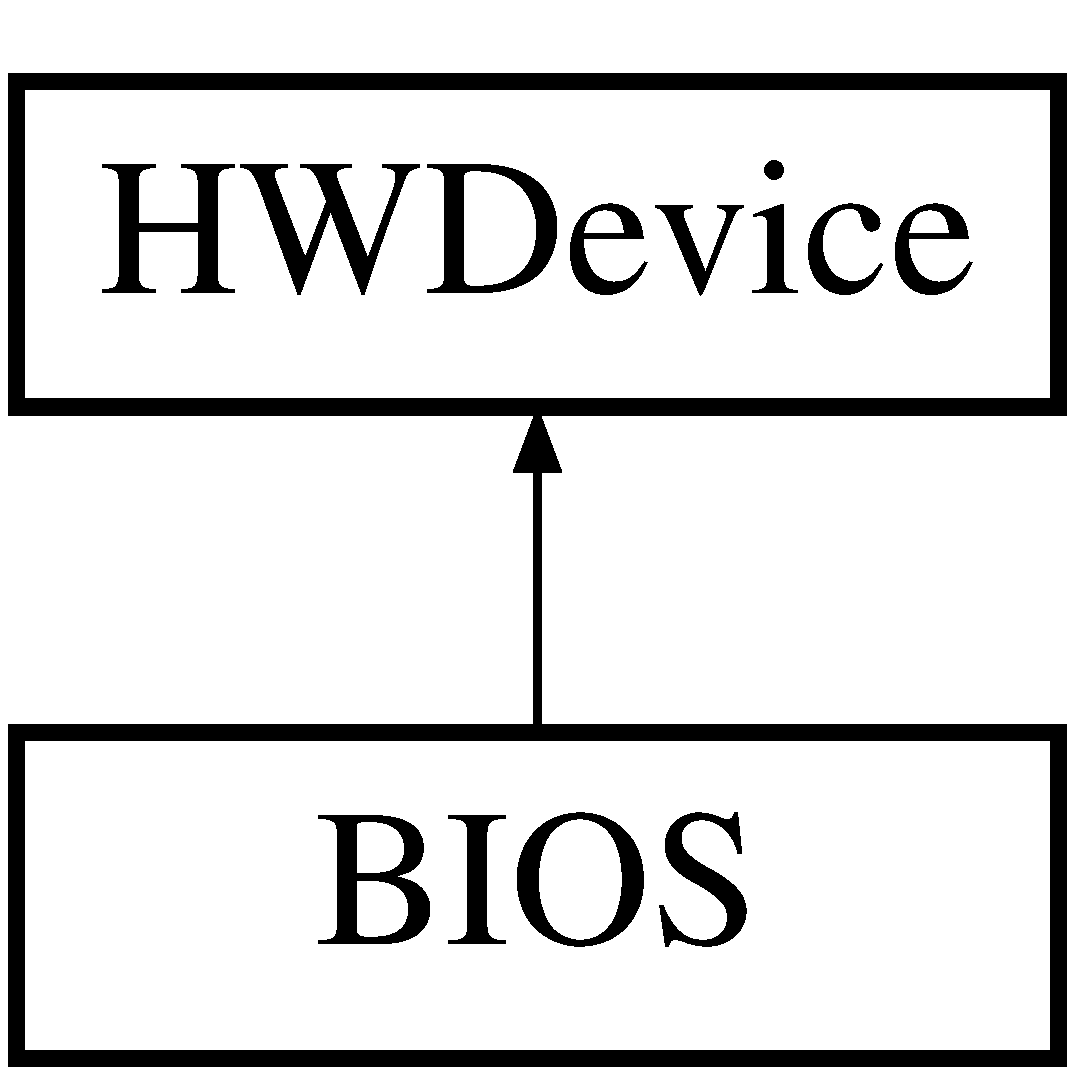
\includegraphics[height=2.000000cm]{classBIOS}
\end{center}
\end{figure}
\subsection*{Public Member Functions}
\begin{DoxyCompactItemize}
\item 
{\bfseries B\+I\+OS} (int position)\hypertarget{classBIOS_adbe126d9247cb1262747f838258bffce}{}\label{classBIOS_adbe126d9247cb1262747f838258bffce}

\end{DoxyCompactItemize}
\subsection*{Additional Inherited Members}


\subsection{Detailed Description}
Rappresents a \hyperlink{classBIOS}{B\+I\+OS} 

The documentation for this class was generated from the following file\+:\begin{DoxyCompactItemize}
\item 
/home/doomdiskday/workspace2/main/src/model/\+H\+W/\+B\+I\+O\+S/B\+I\+O\+S.\+h\end{DoxyCompactItemize}

\hypertarget{classBIOSManager}{}\section{B\+I\+O\+S\+Manager Class Reference}
\label{classBIOSManager}\index{B\+I\+O\+S\+Manager@{B\+I\+O\+S\+Manager}}


{\ttfamily \#include $<$B\+I\+O\+S\+Manager.\+h$>$}

Inheritance diagram for B\+I\+O\+S\+Manager\+:\begin{figure}[H]
\begin{center}
\leavevmode
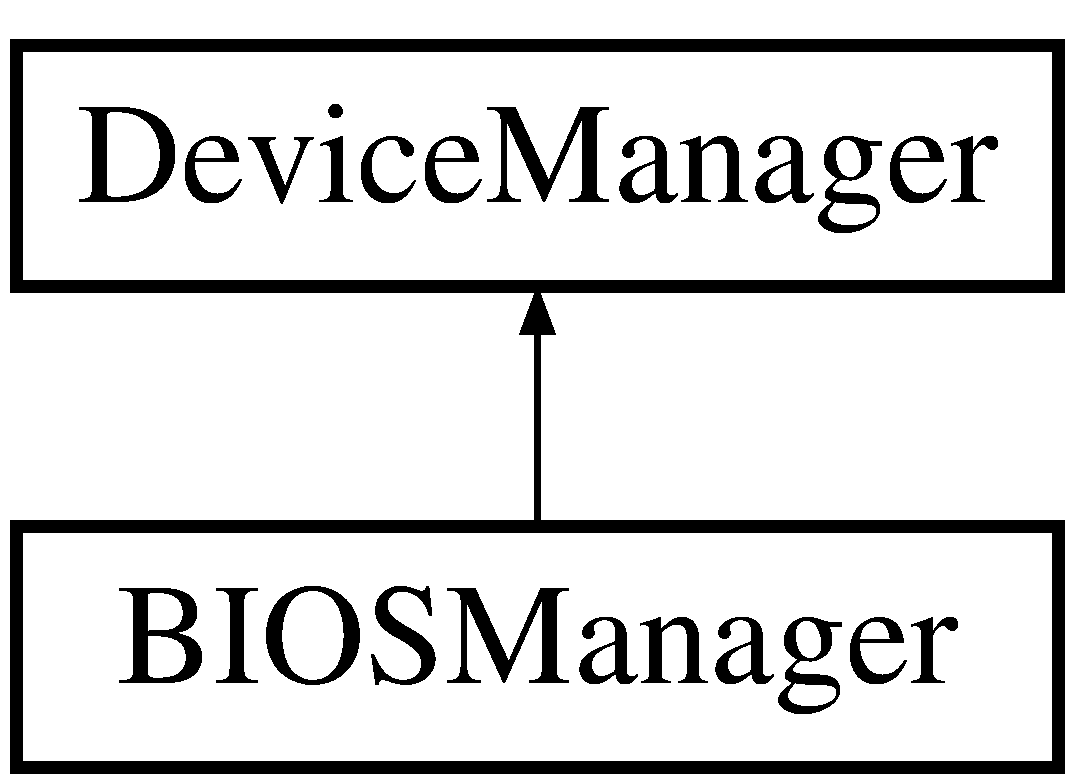
\includegraphics[height=2.000000cm]{classBIOSManager}
\end{center}
\end{figure}
\subsection*{Public Member Functions}
\begin{DoxyCompactItemize}
\item 
void \hyperlink{classBIOSManager_a51496e7da497767975a30fa0aeb53465}{generate\+All\+Devices} ()
\item 
\hyperlink{classHWDevice}{H\+W\+Device} $\ast$ \hyperlink{classBIOSManager_a18f5940451895ec20a049da0b7c01d7d}{generate\+New\+Device} (int position)
\item 
void \hyperlink{classBIOSManager_aaa51bf1d61f4609484a9903fe5a6340e}{set\+Commands} (int device\+Position)
\item 
\hyperlink{classBaseDifference}{Base\+Difference} $\ast$$\ast$ \hyperlink{classBIOSManager_adac6d8eaa4f657834592928b28f29b65}{generate\+Log\+Difference} ()
\item 
\hyperlink{classHWDevice}{H\+W\+Device} $\ast$ \hyperlink{classBIOSManager_ae75fe3a8dad20db9dfa5c3e9ddb2adfd}{generate\+Fake\+Device} ()
\end{DoxyCompactItemize}
\subsection*{Additional Inherited Members}


\subsection{Detailed Description}
This class rappresents a generic \hyperlink{classBIOSManager}{B\+I\+O\+S\+Manager}. It\textquotesingle{}s used to manage all B\+I\+O\+Ses presents on the system. 

\subsection{Member Function Documentation}
\index{B\+I\+O\+S\+Manager@{B\+I\+O\+S\+Manager}!generate\+All\+Devices@{generate\+All\+Devices}}
\index{generate\+All\+Devices@{generate\+All\+Devices}!B\+I\+O\+S\+Manager@{B\+I\+O\+S\+Manager}}
\subsubsection[{\texorpdfstring{generate\+All\+Devices()}{generateAllDevices()}}]{\setlength{\rightskip}{0pt plus 5cm}void B\+I\+O\+S\+Manager\+::generate\+All\+Devices (
\begin{DoxyParamCaption}
{}
\end{DoxyParamCaption}
)\hspace{0.3cm}{\ttfamily [virtual]}}\hypertarget{classBIOSManager_a51496e7da497767975a30fa0aeb53465}{}\label{classBIOSManager_a51496e7da497767975a30fa0aeb53465}
Generate and populate the devices array. This method will be overwritten from the specific classes (\hyperlink{classBIOS}{B\+I\+OS}, H\+DD, ecc..) 

Implements \hyperlink{classDeviceManager_ae9fa3bd3aa66f373d7748628b7ba26cc}{Device\+Manager}.

\index{B\+I\+O\+S\+Manager@{B\+I\+O\+S\+Manager}!generate\+Fake\+Device@{generate\+Fake\+Device}}
\index{generate\+Fake\+Device@{generate\+Fake\+Device}!B\+I\+O\+S\+Manager@{B\+I\+O\+S\+Manager}}
\subsubsection[{\texorpdfstring{generate\+Fake\+Device()}{generateFakeDevice()}}]{\setlength{\rightskip}{0pt plus 5cm}{\bf H\+W\+Device} $\ast$ B\+I\+O\+S\+Manager\+::generate\+Fake\+Device (
\begin{DoxyParamCaption}
{}
\end{DoxyParamCaption}
)\hspace{0.3cm}{\ttfamily [virtual]}}\hypertarget{classBIOSManager_ae75fe3a8dad20db9dfa5c3e9ddb2adfd}{}\label{classBIOSManager_ae75fe3a8dad20db9dfa5c3e9ddb2adfd}
This abstract method will produce a Fake (Specified by the concrete classes) Device that will be used later to compare devices 

Implements \hyperlink{classDeviceManager_a218031345b7b61c79f427985d950c3f3}{Device\+Manager}.

\index{B\+I\+O\+S\+Manager@{B\+I\+O\+S\+Manager}!generate\+Log\+Difference@{generate\+Log\+Difference}}
\index{generate\+Log\+Difference@{generate\+Log\+Difference}!B\+I\+O\+S\+Manager@{B\+I\+O\+S\+Manager}}
\subsubsection[{\texorpdfstring{generate\+Log\+Difference()}{generateLogDifference()}}]{\setlength{\rightskip}{0pt plus 5cm}{\bf Base\+Difference} $\ast$$\ast$ B\+I\+O\+S\+Manager\+::generate\+Log\+Difference (
\begin{DoxyParamCaption}
{}
\end{DoxyParamCaption}
)\hspace{0.3cm}{\ttfamily [virtual]}}\hypertarget{classBIOSManager_adac6d8eaa4f657834592928b28f29b65}{}\label{classBIOSManager_adac6d8eaa4f657834592928b28f29b65}
This abstract method will produce a \hyperlink{classBaseDifference}{Base\+Difference}, it will be used to compare different  between them.

\begin{DoxyReturn}{Returns}
the differences to populate 
\end{DoxyReturn}


Implements \hyperlink{classDeviceManager_ae9916011e50a6a48aea3d87b6c44b27e}{Device\+Manager}.

\index{B\+I\+O\+S\+Manager@{B\+I\+O\+S\+Manager}!generate\+New\+Device@{generate\+New\+Device}}
\index{generate\+New\+Device@{generate\+New\+Device}!B\+I\+O\+S\+Manager@{B\+I\+O\+S\+Manager}}
\subsubsection[{\texorpdfstring{generate\+New\+Device(int position)}{generateNewDevice(int position)}}]{\setlength{\rightskip}{0pt plus 5cm}{\bf H\+W\+Device} $\ast$ B\+I\+O\+S\+Manager\+::generate\+New\+Device (
\begin{DoxyParamCaption}
\item[{int}]{position}
\end{DoxyParamCaption}
)\hspace{0.3cm}{\ttfamily [virtual]}}\hypertarget{classBIOSManager_a18f5940451895ec20a049da0b7c01d7d}{}\label{classBIOSManager_a18f5940451895ec20a049da0b7c01d7d}
Generate and return a new device in a specific position.


\begin{DoxyParams}{Parameters}
{\em position} & used by the device \\
\hline
\end{DoxyParams}
\begin{DoxyReturn}{Returns}
the generated device 
\end{DoxyReturn}


Implements \hyperlink{classDeviceManager_a64c7c17d8cb8d407361dbcf8f6f17ccf}{Device\+Manager}.

\index{B\+I\+O\+S\+Manager@{B\+I\+O\+S\+Manager}!set\+Commands@{set\+Commands}}
\index{set\+Commands@{set\+Commands}!B\+I\+O\+S\+Manager@{B\+I\+O\+S\+Manager}}
\subsubsection[{\texorpdfstring{set\+Commands(int device\+Position)}{setCommands(int devicePosition)}}]{\setlength{\rightskip}{0pt plus 5cm}void B\+I\+O\+S\+Manager\+::set\+Commands (
\begin{DoxyParamCaption}
\item[{int}]{device\+Position}
\end{DoxyParamCaption}
)\hspace{0.3cm}{\ttfamily [virtual]}}\hypertarget{classBIOSManager_aaa51bf1d61f4609484a9903fe5a6340e}{}\label{classBIOSManager_aaa51bf1d61f4609484a9903fe5a6340e}
Set all commands used to retrieve infos. This method will be overwritten from the specific classes (\hyperlink{classBIOS}{B\+I\+OS}, H\+DD, ecc...)


\begin{DoxyParams}{Parameters}
{\em device\+Position} & the device position in the devices array \\
\hline
\end{DoxyParams}


Implements \hyperlink{classDeviceManager_ae367c6847b2988cf6249cbf6254261cb}{Device\+Manager}.



The documentation for this class was generated from the following files\+:\begin{DoxyCompactItemize}
\item 
/home/doomdiskday/workspace2/main/src/model/\+H\+W/\+B\+I\+O\+S/B\+I\+O\+S\+Manager.\+h\item 
/home/doomdiskday/workspace2/main/src/model/\+H\+W/\+B\+I\+O\+S/B\+I\+O\+S\+Manager.\+cpp\end{DoxyCompactItemize}

\hypertarget{classCommand}{}\section{Command Class Reference}
\label{classCommand}\index{Command@{Command}}


{\ttfamily \#include $<$Command.\+h$>$}

\subsection*{Public Member Functions}
\begin{DoxyCompactItemize}
\item 
void {\bfseries set\+Command} (string command)\hypertarget{classCommand_a5939caf9002688381de327a19b7cafae}{}\label{classCommand_a5939caf9002688381de327a19b7cafae}

\item 
void {\bfseries set\+Filter} (string to\+Filter)\hypertarget{classCommand_acf26ff1c38e38207e1522b2d49f0a8b8}{}\label{classCommand_acf26ff1c38e38207e1522b2d49f0a8b8}

\item 
void {\bfseries set\+Second\+Filter} (string second\+Filter)\hypertarget{classCommand_a615bf229502f06c0d5b1a64df7dd1e9c}{}\label{classCommand_a615bf229502f06c0d5b1a64df7dd1e9c}

\item 
int {\bfseries get\+Position} ()\hypertarget{classCommand_ab2573831d9864c076816590bc5a2eb3c}{}\label{classCommand_ab2573831d9864c076816590bc5a2eb3c}

\item 
string {\bfseries get\+Command} ()\hypertarget{classCommand_abdd31f136459c4aeaabcac39ec21bbf1}{}\label{classCommand_abdd31f136459c4aeaabcac39ec21bbf1}

\item 
string {\bfseries get\+Filter} ()\hypertarget{classCommand_a68ab7852a1c55af383220142efce25f3}{}\label{classCommand_a68ab7852a1c55af383220142efce25f3}

\item 
string {\bfseries get\+Second\+Filter} ()\hypertarget{classCommand_a4dedeb327ba2b4439b670d08afdb1286}{}\label{classCommand_a4dedeb327ba2b4439b670d08afdb1286}

\end{DoxyCompactItemize}


\subsection{Detailed Description}
Reppresents a specific command that will be execute to retrieve informations about devices 

The documentation for this class was generated from the following files\+:\begin{DoxyCompactItemize}
\item 
/home/doomdiskday/workspace2/main/src/model/\+H\+W/\+Basic/Command.\+h\item 
/home/doomdiskday/workspace2/main/src/model/\+H\+W/\+Basic/Command.\+cpp\end{DoxyCompactItemize}

\hypertarget{classCommandManager}{}\section{Command\+Manager$<$ T $>$ Class Template Reference}
\label{classCommandManager}\index{Command\+Manager$<$ T $>$@{Command\+Manager$<$ T $>$}}


{\ttfamily \#include $<$Command\+Manager.\+h$>$}

Inheritance diagram for Command\+Manager$<$ T $>$\+:\begin{figure}[H]
\begin{center}
\leavevmode
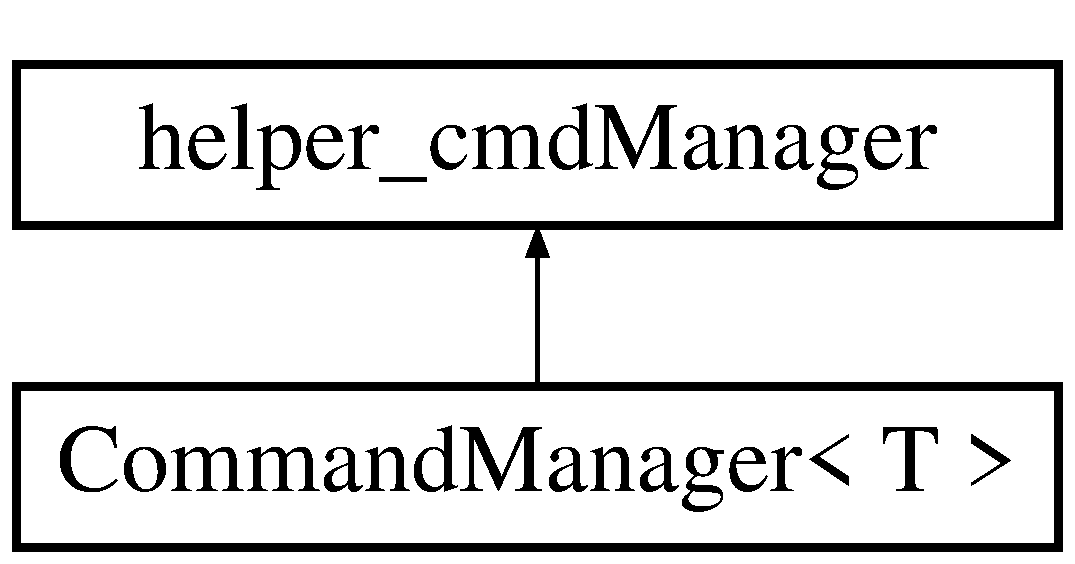
\includegraphics[height=2.000000cm]{classCommandManager}
\end{center}
\end{figure}
\subsection*{Additional Inherited Members}


\subsection{Detailed Description}
\subsubsection*{template$<$class T$>$\\*
class Command\+Manager$<$ T $>$}

Used to manage commands 

The documentation for this class was generated from the following file\+:\begin{DoxyCompactItemize}
\item 
/home/doomdiskday/workspace2/main/src/utils/Command\+Manager.\+h\end{DoxyCompactItemize}

\hypertarget{classCommandManager_3_01int_01_4}{}\section{Command\+Manager$<$ int $>$ Class Template Reference}
\label{classCommandManager_3_01int_01_4}\index{Command\+Manager$<$ int $>$@{Command\+Manager$<$ int $>$}}
Inheritance diagram for Command\+Manager$<$ int $>$\+:\begin{figure}[H]
\begin{center}
\leavevmode
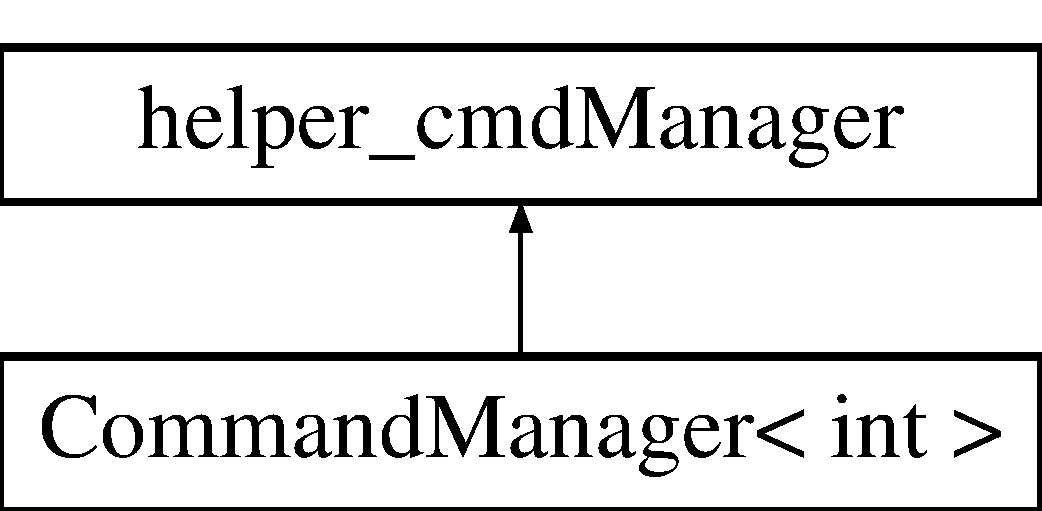
\includegraphics[height=2.000000cm]{classCommandManager_3_01int_01_4}
\end{center}
\end{figure}
\subsection*{Public Member Functions}
\begin{DoxyCompactItemize}
\item 
int {\bfseries get\+Info\+From\+Command} (\hyperlink{classCommand}{Command} $\ast$cmd)\hypertarget{classCommandManager_3_01int_01_4_aa9e1e98538e24030a1d0cdc527066019}{}\label{classCommandManager_3_01int_01_4_aa9e1e98538e24030a1d0cdc527066019}

\end{DoxyCompactItemize}


The documentation for this class was generated from the following file\+:\begin{DoxyCompactItemize}
\item 
/home/doomdiskday/workspace2/main/src/utils/Command\+Manager.\+h\end{DoxyCompactItemize}

\hypertarget{classCommandManager_3_01string_01_4}{}\section{Command\+Manager$<$ string $>$ Class Template Reference}
\label{classCommandManager_3_01string_01_4}\index{Command\+Manager$<$ string $>$@{Command\+Manager$<$ string $>$}}
Inheritance diagram for Command\+Manager$<$ string $>$\+:\begin{figure}[H]
\begin{center}
\leavevmode
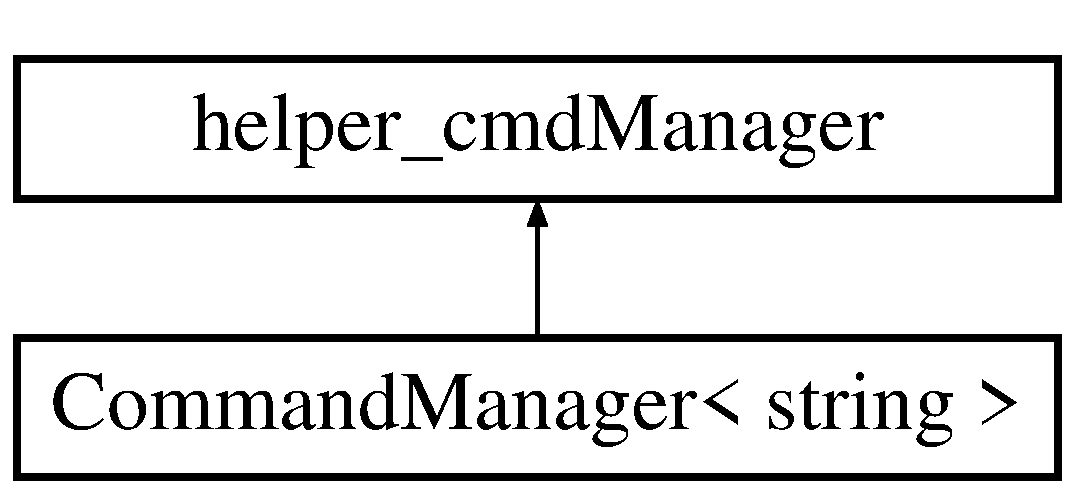
\includegraphics[height=2.000000cm]{classCommandManager_3_01string_01_4}
\end{center}
\end{figure}
\subsection*{Public Member Functions}
\begin{DoxyCompactItemize}
\item 
string {\bfseries get\+Info\+From\+Command} (\hyperlink{classCommand}{Command} $\ast$cmd)\hypertarget{classCommandManager_3_01string_01_4_a78542c11499eae788e790e44a3f5e5c6}{}\label{classCommandManager_3_01string_01_4_a78542c11499eae788e790e44a3f5e5c6}

\end{DoxyCompactItemize}


The documentation for this class was generated from the following file\+:\begin{DoxyCompactItemize}
\item 
/home/doomdiskday/workspace2/main/src/utils/Command\+Manager.\+h\end{DoxyCompactItemize}

\hypertarget{classDeviceManager}{}\section{Device\+Manager Class Reference}
\label{classDeviceManager}\index{Device\+Manager@{Device\+Manager}}


{\ttfamily \#include $<$Device\+Manager.\+h$>$}

Inheritance diagram for Device\+Manager\+:\begin{figure}[H]
\begin{center}
\leavevmode
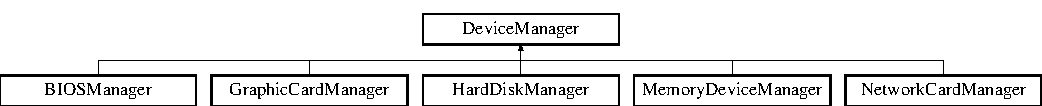
\includegraphics[height=1.426752cm]{classDeviceManager}
\end{center}
\end{figure}
\subsection*{Public Member Functions}
\begin{DoxyCompactItemize}
\item 
int \hyperlink{classDeviceManager_ab0e75c9472f3213243f5be200cf8a459}{get\+Number\+Of\+Devices} ()
\item 
\hyperlink{classHWDevice}{H\+W\+Device} $\ast$$\ast$ \hyperlink{classDeviceManager_a6d01b46c8522dc3d5a7cefbab539a21d}{get\+Devices} ()
\item 
string \hyperlink{classDeviceManager_aebc35de93caa9623ac28166f463494fb}{get\+File\+Path} ()
\item 
void \hyperlink{classDeviceManager_ac5ebb7ae4c669b43e96f2c533880c2a2}{print\+All\+Infos} ()
\item 
virtual bool \hyperlink{classDeviceManager_af9949548d51650ab8ac223d32559f8f0}{check\+Devices\+Existence} ()
\item 
virtual void \hyperlink{classDeviceManager_ae9fa3bd3aa66f373d7748628b7ba26cc}{generate\+All\+Devices} ()=0
\item 
virtual \hyperlink{classHWDevice}{H\+W\+Device} $\ast$ \hyperlink{classDeviceManager_a64c7c17d8cb8d407361dbcf8f6f17ccf}{generate\+New\+Device} (int position)=0
\item 
virtual void \hyperlink{classDeviceManager_ae367c6847b2988cf6249cbf6254261cb}{set\+Commands} (int device\+Position)=0
\item 
virtual void \hyperlink{classDeviceManager_a4c34a8b9035b29829739c533b611ab07}{set\+All\+Infos} (int position)
\item 
virtual void \hyperlink{classDeviceManager_a17458750431e2131c06e58e8b82a90d1}{find\+Devices} ()
\item 
virtual void \hyperlink{classDeviceManager_a0bbabbb33adf1eb6eee22ac78d1da7b7}{generate\+Log} ()
\item 
int \hyperlink{classDeviceManager_a7e7bcbfe9ad42a5986d354352b80d917}{count\+Devices\+From\+File} (string path)
\item 
\hyperlink{classHWDevice}{H\+W\+Device} $\ast$$\ast$ \hyperlink{classDeviceManager_a8c9576d042fb3a949c7658bb514a54ae}{retrieve\+From\+File} (string path, int \&err, int \&size)
\item 
virtual \hyperlink{classBaseDifference}{Base\+Difference} $\ast$$\ast$ \hyperlink{classDeviceManager_ae9916011e50a6a48aea3d87b6c44b27e}{generate\+Log\+Difference} ()=0
\item 
virtual \hyperlink{classHWDevice}{H\+W\+Device} $\ast$ \hyperlink{classDeviceManager_a218031345b7b61c79f427985d950c3f3}{generate\+Fake\+Device} ()=0
\item 
\hyperlink{classBaseDifference}{Base\+Difference} $\ast$$\ast$ \hyperlink{classDeviceManager_a2e15cd9f0728183029e9d078c942da0a}{check\+Devices} (\hyperlink{classHWDevice}{H\+W\+Device} $\ast$orig, \hyperlink{classHWDevice}{H\+W\+Device} $\ast$to\+Check)
\item 
\hyperlink{classBaseDifference}{Base\+Difference} $\ast$$\ast$$\ast$ \hyperlink{classDeviceManager_a571878f54147f206f63aad938fb59b51}{check\+Devices\+From\+File} (string path, int \&err, int \&size, int \&added, int \&removed)
\end{DoxyCompactItemize}
\subsection*{Protected Attributes}
\begin{DoxyCompactItemize}
\item 
string {\bfseries file\+Name}\hypertarget{classDeviceManager_a744ce0aeda4453860233c6f8b5adb3d4}{}\label{classDeviceManager_a744ce0aeda4453860233c6f8b5adb3d4}

\item 
string {\bfseries in\+File\+Name}\hypertarget{classDeviceManager_a4b4f8ded511116ad9247f9dff8e52276}{}\label{classDeviceManager_a4b4f8ded511116ad9247f9dff8e52276}

\item 
string {\bfseries on\+Difference\+Name}\hypertarget{classDeviceManager_a0ec69b1c6c309a18c35c929a8270de8e}{}\label{classDeviceManager_a0ec69b1c6c309a18c35c929a8270de8e}

\item 
int {\bfseries number\+Of\+Infos}\hypertarget{classDeviceManager_a423e58bd66300388667857304f89f488}{}\label{classDeviceManager_a423e58bd66300388667857304f89f488}

\item 
\hyperlink{classCommand}{Command} $\ast$ {\bfseries number\+Of\+Devices\+Command}\hypertarget{classDeviceManager_a2494b9606c93ee9fb33e32594fa575bf}{}\label{classDeviceManager_a2494b9606c93ee9fb33e32594fa575bf}

\item 
int {\bfseries number\+Of\+Devices}\hypertarget{classDeviceManager_a0d1b28c1d0439fed7c41a15974860697}{}\label{classDeviceManager_a0d1b28c1d0439fed7c41a15974860697}

\item 
\hyperlink{classHWDevice}{H\+W\+Device} $\ast$$\ast$ {\bfseries devices}\hypertarget{classDeviceManager_ac6a7ba09f929d09fbabf60d36db24b2c}{}\label{classDeviceManager_ac6a7ba09f929d09fbabf60d36db24b2c}

\item 
\hyperlink{classCommand}{Command} $\ast$$\ast$ {\bfseries commands}\hypertarget{classDeviceManager_a0f68f691cc8127b0eac36b3e4b2603fd}{}\label{classDeviceManager_a0f68f691cc8127b0eac36b3e4b2603fd}

\item 
int {\bfseries number\+Of\+Commands}\hypertarget{classDeviceManager_a6740c39443b17dc714bebd8b76c201d4}{}\label{classDeviceManager_a6740c39443b17dc714bebd8b76c201d4}

\item 
\hyperlink{classCommand}{Command} $\ast$ {\bfseries check\+Command}\hypertarget{classDeviceManager_abd465cbbacdcfdbe5c91afb365549b92}{}\label{classDeviceManager_abd465cbbacdcfdbe5c91afb365549b92}

\end{DoxyCompactItemize}
\subsection*{Friends}
\begin{DoxyCompactItemize}
\item 
class {\bfseries H\+W\+Manager}\hypertarget{classDeviceManager_abb119eaaf520facbb8c60125012911a2}{}\label{classDeviceManager_abb119eaaf520facbb8c60125012911a2}

\end{DoxyCompactItemize}


\subsection{Detailed Description}
Abstract class used to manage completely a group of specific  

\subsection{Member Function Documentation}
\index{Device\+Manager@{Device\+Manager}!check\+Devices@{check\+Devices}}
\index{check\+Devices@{check\+Devices}!Device\+Manager@{Device\+Manager}}
\subsubsection[{\texorpdfstring{check\+Devices(\+H\+W\+Device $\ast$orig, H\+W\+Device $\ast$to\+Check)}{checkDevices(HWDevice *orig, HWDevice *toCheck)}}]{\setlength{\rightskip}{0pt plus 5cm}{\bf Base\+Difference}$\ast$$\ast$ Device\+Manager\+::check\+Devices (
\begin{DoxyParamCaption}
\item[{{\bf H\+W\+Device} $\ast$}]{orig, }
\item[{{\bf H\+W\+Device} $\ast$}]{to\+Check}
\end{DoxyParamCaption}
)\hspace{0.3cm}{\ttfamily [inline]}}\hypertarget{classDeviceManager_a2e15cd9f0728183029e9d078c942da0a}{}\label{classDeviceManager_a2e15cd9f0728183029e9d078c942da0a}
This method check two different  between them and return a difference log. \index{Device\+Manager@{Device\+Manager}!check\+Devices\+Existence@{check\+Devices\+Existence}}
\index{check\+Devices\+Existence@{check\+Devices\+Existence}!Device\+Manager@{Device\+Manager}}
\subsubsection[{\texorpdfstring{check\+Devices\+Existence()}{checkDevicesExistence()}}]{\setlength{\rightskip}{0pt plus 5cm}virtual bool Device\+Manager\+::check\+Devices\+Existence (
\begin{DoxyParamCaption}
{}
\end{DoxyParamCaption}
)\hspace{0.3cm}{\ttfamily [inline]}, {\ttfamily [virtual]}}\hypertarget{classDeviceManager_af9949548d51650ab8ac223d32559f8f0}{}\label{classDeviceManager_af9949548d51650ab8ac223d32559f8f0}
Check the existences of a specific device.

\begin{DoxyReturn}{Returns}
true if some device exists, false otherwise 
\end{DoxyReturn}
\index{Device\+Manager@{Device\+Manager}!check\+Devices\+From\+File@{check\+Devices\+From\+File}}
\index{check\+Devices\+From\+File@{check\+Devices\+From\+File}!Device\+Manager@{Device\+Manager}}
\subsubsection[{\texorpdfstring{check\+Devices\+From\+File(string path, int \&err, int \&size, int \&added, int \&removed)}{checkDevicesFromFile(string path, int &err, int &size, int &added, int &removed)}}]{\setlength{\rightskip}{0pt plus 5cm}{\bf Base\+Difference}$\ast$$\ast$$\ast$ Device\+Manager\+::check\+Devices\+From\+File (
\begin{DoxyParamCaption}
\item[{string}]{path, }
\item[{int \&}]{err, }
\item[{int \&}]{size, }
\item[{int \&}]{added, }
\item[{int \&}]{removed}
\end{DoxyParamCaption}
)\hspace{0.3cm}{\ttfamily [inline]}}\hypertarget{classDeviceManager_a571878f54147f206f63aad938fb59b51}{}\label{classDeviceManager_a571878f54147f206f63aad938fb59b51}
This method checks devices retrieved on the machine with a well-\/formed log passed by param.


\begin{DoxyParams}{Parameters}
{\em path} & log file path \\
\hline
{\em err} & error message (0 = OK, -\/1 = S\+O\+M\+E\+T\+H\+I\+NG W\+E\+NT W\+R\+O\+NG) \\
\hline
{\em size} & difference log size \\
\hline
{\em added} & number of devices apparently added \\
\hline
{\em removed} & number of devices apparently removed \\
\hline
\end{DoxyParams}
\index{Device\+Manager@{Device\+Manager}!count\+Devices\+From\+File@{count\+Devices\+From\+File}}
\index{count\+Devices\+From\+File@{count\+Devices\+From\+File}!Device\+Manager@{Device\+Manager}}
\subsubsection[{\texorpdfstring{count\+Devices\+From\+File(string path)}{countDevicesFromFile(string path)}}]{\setlength{\rightskip}{0pt plus 5cm}int Device\+Manager\+::count\+Devices\+From\+File (
\begin{DoxyParamCaption}
\item[{string}]{path}
\end{DoxyParamCaption}
)\hspace{0.3cm}{\ttfamily [inline]}}\hypertarget{classDeviceManager_a7e7bcbfe9ad42a5986d354352b80d917}{}\label{classDeviceManager_a7e7bcbfe9ad42a5986d354352b80d917}
Return the number of devices retrieved in a log\+File.


\begin{DoxyParams}{Parameters}
{\em path} & the log file path \\
\hline
\end{DoxyParams}
\begin{DoxyReturn}{Returns}
number of devices retrieved in a file 
\end{DoxyReturn}
\index{Device\+Manager@{Device\+Manager}!find\+Devices@{find\+Devices}}
\index{find\+Devices@{find\+Devices}!Device\+Manager@{Device\+Manager}}
\subsubsection[{\texorpdfstring{find\+Devices()}{findDevices()}}]{\setlength{\rightskip}{0pt plus 5cm}virtual void Device\+Manager\+::find\+Devices (
\begin{DoxyParamCaption}
{}
\end{DoxyParamCaption}
)\hspace{0.3cm}{\ttfamily [inline]}, {\ttfamily [virtual]}}\hypertarget{classDeviceManager_a17458750431e2131c06e58e8b82a90d1}{}\label{classDeviceManager_a17458750431e2131c06e58e8b82a90d1}
Find all devices in the system and set it the devices array of the class \index{Device\+Manager@{Device\+Manager}!generate\+All\+Devices@{generate\+All\+Devices}}
\index{generate\+All\+Devices@{generate\+All\+Devices}!Device\+Manager@{Device\+Manager}}
\subsubsection[{\texorpdfstring{generate\+All\+Devices()=0}{generateAllDevices()=0}}]{\setlength{\rightskip}{0pt plus 5cm}virtual void Device\+Manager\+::generate\+All\+Devices (
\begin{DoxyParamCaption}
{}
\end{DoxyParamCaption}
)\hspace{0.3cm}{\ttfamily [pure virtual]}}\hypertarget{classDeviceManager_ae9fa3bd3aa66f373d7748628b7ba26cc}{}\label{classDeviceManager_ae9fa3bd3aa66f373d7748628b7ba26cc}
Generate and populate the devices array. This method will be overwritten from the specific classes (\hyperlink{classBIOS}{B\+I\+OS}, H\+DD, ecc..) 

Implemented in \hyperlink{classMemoryDeviceManager_a84565386d5d9ada62c495558ba7c06f8}{Memory\+Device\+Manager}, \hyperlink{classNetworkCardManager_aa6a77a00f2366720ef0a4cbbe5c01a1d}{Network\+Card\+Manager}, \hyperlink{classBIOSManager_a51496e7da497767975a30fa0aeb53465}{B\+I\+O\+S\+Manager}, \hyperlink{classHardDiskManager_ac69f4cfc902fa23ff238f33ee9731c3c}{Hard\+Disk\+Manager}, and \hyperlink{classGraphicCardManager_a6c94b17b01bd0f27bf0822c269d1c41c}{Graphic\+Card\+Manager}.

\index{Device\+Manager@{Device\+Manager}!generate\+Fake\+Device@{generate\+Fake\+Device}}
\index{generate\+Fake\+Device@{generate\+Fake\+Device}!Device\+Manager@{Device\+Manager}}
\subsubsection[{\texorpdfstring{generate\+Fake\+Device()=0}{generateFakeDevice()=0}}]{\setlength{\rightskip}{0pt plus 5cm}virtual {\bf H\+W\+Device}$\ast$ Device\+Manager\+::generate\+Fake\+Device (
\begin{DoxyParamCaption}
{}
\end{DoxyParamCaption}
)\hspace{0.3cm}{\ttfamily [pure virtual]}}\hypertarget{classDeviceManager_a218031345b7b61c79f427985d950c3f3}{}\label{classDeviceManager_a218031345b7b61c79f427985d950c3f3}
This abstract method will produce a Fake (Specified by the concrete classes) Device that will be used later to compare devices 

Implemented in \hyperlink{classNetworkCardManager_a473a9578d17f85f125183a6c48f86eb8}{Network\+Card\+Manager}, \hyperlink{classMemoryDeviceManager_aa652b05bfea23ce4dbe562ed158fb165}{Memory\+Device\+Manager}, \hyperlink{classHardDiskManager_a586e786b4512ec8dfb79edb743794b77}{Hard\+Disk\+Manager}, \hyperlink{classBIOSManager_ae75fe3a8dad20db9dfa5c3e9ddb2adfd}{B\+I\+O\+S\+Manager}, and \hyperlink{classGraphicCardManager_ac71590c819520e60a491c8e69252efe1}{Graphic\+Card\+Manager}.

\index{Device\+Manager@{Device\+Manager}!generate\+Log@{generate\+Log}}
\index{generate\+Log@{generate\+Log}!Device\+Manager@{Device\+Manager}}
\subsubsection[{\texorpdfstring{generate\+Log()}{generateLog()}}]{\setlength{\rightskip}{0pt plus 5cm}virtual void Device\+Manager\+::generate\+Log (
\begin{DoxyParamCaption}
{}
\end{DoxyParamCaption}
)\hspace{0.3cm}{\ttfamily [inline]}, {\ttfamily [virtual]}}\hypertarget{classDeviceManager_a0bbabbb33adf1eb6eee22ac78d1da7b7}{}\label{classDeviceManager_a0bbabbb33adf1eb6eee22ac78d1da7b7}
Generate a log under the file\+Name path. This method iterate for each device and visit each information with a visitor able to log them. \index{Device\+Manager@{Device\+Manager}!generate\+Log\+Difference@{generate\+Log\+Difference}}
\index{generate\+Log\+Difference@{generate\+Log\+Difference}!Device\+Manager@{Device\+Manager}}
\subsubsection[{\texorpdfstring{generate\+Log\+Difference()=0}{generateLogDifference()=0}}]{\setlength{\rightskip}{0pt plus 5cm}virtual {\bf Base\+Difference}$\ast$$\ast$ Device\+Manager\+::generate\+Log\+Difference (
\begin{DoxyParamCaption}
{}
\end{DoxyParamCaption}
)\hspace{0.3cm}{\ttfamily [pure virtual]}}\hypertarget{classDeviceManager_ae9916011e50a6a48aea3d87b6c44b27e}{}\label{classDeviceManager_ae9916011e50a6a48aea3d87b6c44b27e}
This abstract method will produce a \hyperlink{classBaseDifference}{Base\+Difference}, it will be used to compare different  between them.

\begin{DoxyReturn}{Returns}
the differences to populate 
\end{DoxyReturn}


Implemented in \hyperlink{classNetworkCardManager_a8dc8b4267433e57c6450fb7ebb0a43f6}{Network\+Card\+Manager}, \hyperlink{classMemoryDeviceManager_a1462e426adfe44f815359fb7f8b096b1}{Memory\+Device\+Manager}, \hyperlink{classHardDiskManager_ae8579afefc3c0619ef05c30b9fda3b82}{Hard\+Disk\+Manager}, \hyperlink{classBIOSManager_adac6d8eaa4f657834592928b28f29b65}{B\+I\+O\+S\+Manager}, and \hyperlink{classGraphicCardManager_a17d988dac37f04cb1dddd45eef8c3aea}{Graphic\+Card\+Manager}.

\index{Device\+Manager@{Device\+Manager}!generate\+New\+Device@{generate\+New\+Device}}
\index{generate\+New\+Device@{generate\+New\+Device}!Device\+Manager@{Device\+Manager}}
\subsubsection[{\texorpdfstring{generate\+New\+Device(int position)=0}{generateNewDevice(int position)=0}}]{\setlength{\rightskip}{0pt plus 5cm}virtual {\bf H\+W\+Device}$\ast$ Device\+Manager\+::generate\+New\+Device (
\begin{DoxyParamCaption}
\item[{int}]{position}
\end{DoxyParamCaption}
)\hspace{0.3cm}{\ttfamily [pure virtual]}}\hypertarget{classDeviceManager_a64c7c17d8cb8d407361dbcf8f6f17ccf}{}\label{classDeviceManager_a64c7c17d8cb8d407361dbcf8f6f17ccf}
Generate and return a new device in a specific position.


\begin{DoxyParams}{Parameters}
{\em position} & used by the device \\
\hline
\end{DoxyParams}
\begin{DoxyReturn}{Returns}
the generated device 
\end{DoxyReturn}


Implemented in \hyperlink{classMemoryDeviceManager_a2fa6b078f50c4bfbbbef218b8289ee89}{Memory\+Device\+Manager}, \hyperlink{classNetworkCardManager_a675dcf10689da520c3ab5ff32d066811}{Network\+Card\+Manager}, \hyperlink{classBIOSManager_a18f5940451895ec20a049da0b7c01d7d}{B\+I\+O\+S\+Manager}, \hyperlink{classHardDiskManager_a3960650a3232567f3488fb10fb10fa7c}{Hard\+Disk\+Manager}, and \hyperlink{classGraphicCardManager_a1835a9054bccb574e74dc2ebb2c28554}{Graphic\+Card\+Manager}.

\index{Device\+Manager@{Device\+Manager}!get\+Devices@{get\+Devices}}
\index{get\+Devices@{get\+Devices}!Device\+Manager@{Device\+Manager}}
\subsubsection[{\texorpdfstring{get\+Devices()}{getDevices()}}]{\setlength{\rightskip}{0pt plus 5cm}{\bf H\+W\+Device}$\ast$$\ast$ Device\+Manager\+::get\+Devices (
\begin{DoxyParamCaption}
{}
\end{DoxyParamCaption}
)\hspace{0.3cm}{\ttfamily [inline]}}\hypertarget{classDeviceManager_a6d01b46c8522dc3d5a7cefbab539a21d}{}\label{classDeviceManager_a6d01b46c8522dc3d5a7cefbab539a21d}
Return the devices array

\begin{DoxyReturn}{Returns}
devices array 
\end{DoxyReturn}
\index{Device\+Manager@{Device\+Manager}!get\+File\+Path@{get\+File\+Path}}
\index{get\+File\+Path@{get\+File\+Path}!Device\+Manager@{Device\+Manager}}
\subsubsection[{\texorpdfstring{get\+File\+Path()}{getFilePath()}}]{\setlength{\rightskip}{0pt plus 5cm}string Device\+Manager\+::get\+File\+Path (
\begin{DoxyParamCaption}
{}
\end{DoxyParamCaption}
)\hspace{0.3cm}{\ttfamily [inline]}}\hypertarget{classDeviceManager_aebc35de93caa9623ac28166f463494fb}{}\label{classDeviceManager_aebc35de93caa9623ac28166f463494fb}
Return the file path \index{Device\+Manager@{Device\+Manager}!get\+Number\+Of\+Devices@{get\+Number\+Of\+Devices}}
\index{get\+Number\+Of\+Devices@{get\+Number\+Of\+Devices}!Device\+Manager@{Device\+Manager}}
\subsubsection[{\texorpdfstring{get\+Number\+Of\+Devices()}{getNumberOfDevices()}}]{\setlength{\rightskip}{0pt plus 5cm}int Device\+Manager\+::get\+Number\+Of\+Devices (
\begin{DoxyParamCaption}
{}
\end{DoxyParamCaption}
)\hspace{0.3cm}{\ttfamily [inline]}}\hypertarget{classDeviceManager_ab0e75c9472f3213243f5be200cf8a459}{}\label{classDeviceManager_ab0e75c9472f3213243f5be200cf8a459}
Return the number of devices

\begin{DoxyReturn}{Returns}
number of devices 
\end{DoxyReturn}
\index{Device\+Manager@{Device\+Manager}!print\+All\+Infos@{print\+All\+Infos}}
\index{print\+All\+Infos@{print\+All\+Infos}!Device\+Manager@{Device\+Manager}}
\subsubsection[{\texorpdfstring{print\+All\+Infos()}{printAllInfos()}}]{\setlength{\rightskip}{0pt plus 5cm}void Device\+Manager\+::print\+All\+Infos (
\begin{DoxyParamCaption}
{}
\end{DoxyParamCaption}
)\hspace{0.3cm}{\ttfamily [inline]}}\hypertarget{classDeviceManager_ac5ebb7ae4c669b43e96f2c533880c2a2}{}\label{classDeviceManager_ac5ebb7ae4c669b43e96f2c533880c2a2}
Print all infos about devices with the following format\+: P\+R\+O\+P\+E\+R\+TY \+: V\+A\+L\+UE \index{Device\+Manager@{Device\+Manager}!retrieve\+From\+File@{retrieve\+From\+File}}
\index{retrieve\+From\+File@{retrieve\+From\+File}!Device\+Manager@{Device\+Manager}}
\subsubsection[{\texorpdfstring{retrieve\+From\+File(string path, int \&err, int \&size)}{retrieveFromFile(string path, int &err, int &size)}}]{\setlength{\rightskip}{0pt plus 5cm}{\bf H\+W\+Device}$\ast$$\ast$ Device\+Manager\+::retrieve\+From\+File (
\begin{DoxyParamCaption}
\item[{string}]{path, }
\item[{int \&}]{err, }
\item[{int \&}]{size}
\end{DoxyParamCaption}
)\hspace{0.3cm}{\ttfamily [inline]}}\hypertarget{classDeviceManager_a8c9576d042fb3a949c7658bb514a54ae}{}\label{classDeviceManager_a8c9576d042fb3a949c7658bb514a54ae}
Return an H\+W\+Device$\ast$ array from a log file passed as parameter.


\begin{DoxyParams}{Parameters}
{\em path} & the log file path \\
\hline
{\em err} & errors\mbox{[} 0 = OK, 1 = NO D\+E\+V\+I\+C\+ES F\+O\+U\+ND\mbox{]} \\
\hline
{\em size} & the output array size \\
\hline
\end{DoxyParams}
\begin{DoxyReturn}{Returns}
H\+W\+Device$\ast$ array 
\end{DoxyReturn}
\index{Device\+Manager@{Device\+Manager}!set\+All\+Infos@{set\+All\+Infos}}
\index{set\+All\+Infos@{set\+All\+Infos}!Device\+Manager@{Device\+Manager}}
\subsubsection[{\texorpdfstring{set\+All\+Infos(int position)}{setAllInfos(int position)}}]{\setlength{\rightskip}{0pt plus 5cm}virtual void Device\+Manager\+::set\+All\+Infos (
\begin{DoxyParamCaption}
\item[{int}]{position}
\end{DoxyParamCaption}
)\hspace{0.3cm}{\ttfamily [inline]}, {\ttfamily [virtual]}}\hypertarget{classDeviceManager_a4c34a8b9035b29829739c533b611ab07}{}\label{classDeviceManager_a4c34a8b9035b29829739c533b611ab07}
Set all devices informations, by default this method set all properties using the commands array and pass it, with a visitor, to the property


\begin{DoxyParams}{Parameters}
{\em position} & the device position in the device array \\
\hline
\end{DoxyParams}


Reimplemented in \hyperlink{classNetworkCardManager_a880800c63daa416ec642691c0d85ca4a}{Network\+Card\+Manager}.

\index{Device\+Manager@{Device\+Manager}!set\+Commands@{set\+Commands}}
\index{set\+Commands@{set\+Commands}!Device\+Manager@{Device\+Manager}}
\subsubsection[{\texorpdfstring{set\+Commands(int device\+Position)=0}{setCommands(int devicePosition)=0}}]{\setlength{\rightskip}{0pt plus 5cm}virtual void Device\+Manager\+::set\+Commands (
\begin{DoxyParamCaption}
\item[{int}]{device\+Position}
\end{DoxyParamCaption}
)\hspace{0.3cm}{\ttfamily [pure virtual]}}\hypertarget{classDeviceManager_ae367c6847b2988cf6249cbf6254261cb}{}\label{classDeviceManager_ae367c6847b2988cf6249cbf6254261cb}
Set all commands used to retrieve infos. This method will be overwritten from the specific classes (\hyperlink{classBIOS}{B\+I\+OS}, H\+DD, ecc...)


\begin{DoxyParams}{Parameters}
{\em device\+Position} & the device position in the devices array \\
\hline
\end{DoxyParams}


Implemented in \hyperlink{classMemoryDeviceManager_a0246a46d583a717dfabc625a5e387400}{Memory\+Device\+Manager}, \hyperlink{classNetworkCardManager_a9204cc788a83cafc73b2f798963417a2}{Network\+Card\+Manager}, \hyperlink{classBIOSManager_aaa51bf1d61f4609484a9903fe5a6340e}{B\+I\+O\+S\+Manager}, \hyperlink{classHardDiskManager_a8e219e6e508dd2d8a6190c44bcf45782}{Hard\+Disk\+Manager}, and \hyperlink{classGraphicCardManager_a42bc616062f94b2e4ee92a79ba537a16}{Graphic\+Card\+Manager}.



The documentation for this class was generated from the following file\+:\begin{DoxyCompactItemize}
\item 
/home/doomdiskday/workspace2/main/src/model/\+H\+W/\+Basic/Device\+Manager.\+h\end{DoxyCompactItemize}

\hypertarget{classFirmware}{}\section{Firmware Class Reference}
\label{classFirmware}\index{Firmware@{Firmware}}
\subsection*{Public Member Functions}
\begin{DoxyCompactItemize}
\item 
void {\bfseries set\+File\+Name} (string file\+\_\+name)\hypertarget{classFirmware_ab4a17f3cb1f104c87cf908fa2322bcb9}{}\label{classFirmware_ab4a17f3cb1f104c87cf908fa2322bcb9}

\item 
void {\bfseries set\+S\+H\+A256} (string sha256)\hypertarget{classFirmware_afafe8f4d217602d499424fa72bafe358}{}\label{classFirmware_afafe8f4d217602d499424fa72bafe358}

\item 
string {\bfseries get\+File\+Name} ()\hypertarget{classFirmware_a2ce07ffdb3f242a32db55437c464effa}{}\label{classFirmware_a2ce07ffdb3f242a32db55437c464effa}

\item 
string {\bfseries get\+S\+H\+A256} ()\hypertarget{classFirmware_a8cb04f299dc56f6a4787c3efd52aace0}{}\label{classFirmware_a8cb04f299dc56f6a4787c3efd52aace0}

\end{DoxyCompactItemize}


The documentation for this class was generated from the following file\+:\begin{DoxyCompactItemize}
\item 
/home/doomdiskday/workspace2/main/src/model/\+F\+W/\+Basic/Firmware.\+h\end{DoxyCompactItemize}

\hypertarget{classFirmwareManager}{}\section{Firmware\+Manager Class Reference}
\label{classFirmwareManager}\index{Firmware\+Manager@{Firmware\+Manager}}
\subsection*{Public Member Functions}
\begin{DoxyCompactItemize}
\item 
void {\bfseries find\+Firmware} ()\hypertarget{classFirmwareManager_ac342c3efab95288ed5cd58d4dc55828f}{}\label{classFirmwareManager_ac342c3efab95288ed5cd58d4dc55828f}

\item 
void {\bfseries generate\+Log} ()\hypertarget{classFirmwareManager_a521978f262cfa7ed05a37f73436ac035}{}\label{classFirmwareManager_a521978f262cfa7ed05a37f73436ac035}

\item 
\hyperlink{classFirmware}{Firmware} $\ast$$\ast$ {\bfseries retrieve\+From\+File} (string path, int \&err, int \&size)\hypertarget{classFirmwareManager_ade8c285cc39fa2730541a458cef43123}{}\label{classFirmwareManager_ade8c285cc39fa2730541a458cef43123}

\end{DoxyCompactItemize}


The documentation for this class was generated from the following files\+:\begin{DoxyCompactItemize}
\item 
/home/doomdiskday/workspace2/main/src/model/\+F\+W/\+Manager/Firmware\+Manager.\+h\item 
/home/doomdiskday/workspace2/main/src/model/\+F\+W/\+Manager/Firmware\+Manager.\+cpp\end{DoxyCompactItemize}

\hypertarget{classGraphicCard}{}\section{Graphic\+Card Class Reference}
\label{classGraphicCard}\index{Graphic\+Card@{Graphic\+Card}}


{\ttfamily \#include $<$Graphic\+Card.\+h$>$}

Inheritance diagram for Graphic\+Card\+:\begin{figure}[H]
\begin{center}
\leavevmode
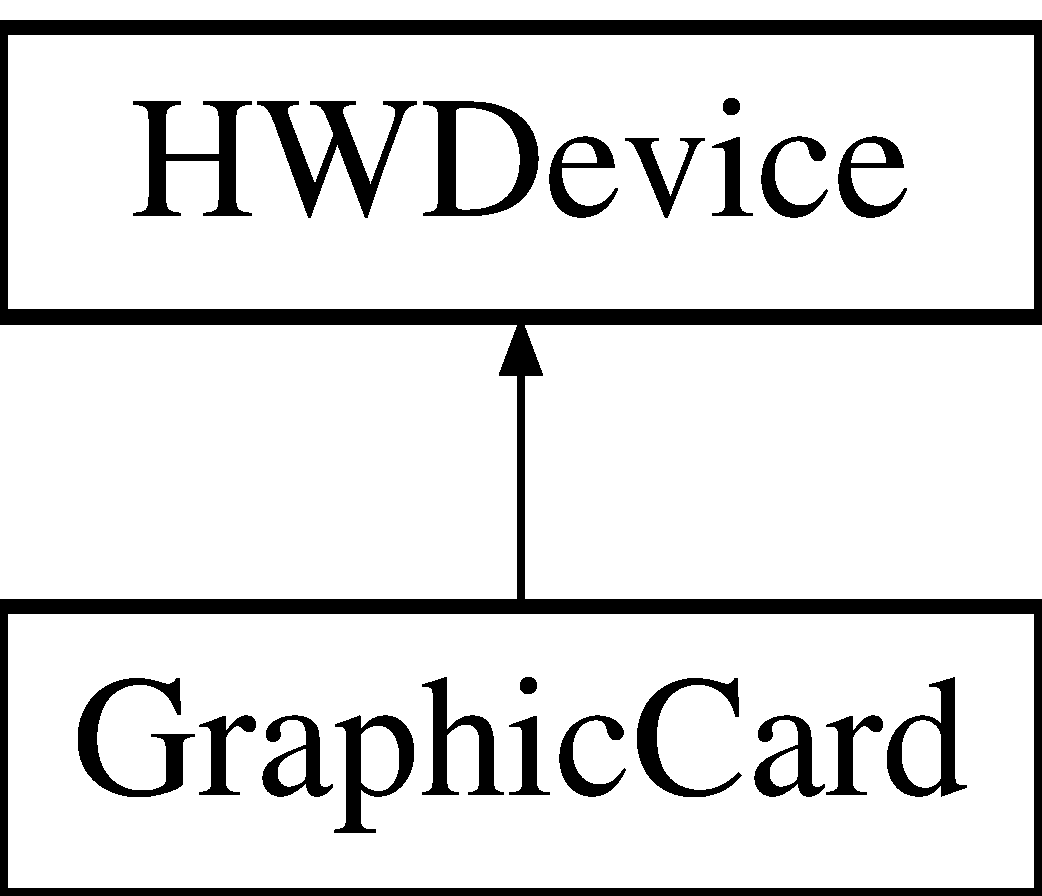
\includegraphics[height=2.000000cm]{classGraphicCard}
\end{center}
\end{figure}
\subsection*{Public Member Functions}
\begin{DoxyCompactItemize}
\item 
{\bfseries Graphic\+Card} (int position)\hypertarget{classGraphicCard_a340281cb1771cdf4006a03e5902fa991}{}\label{classGraphicCard_a340281cb1771cdf4006a03e5902fa991}

\end{DoxyCompactItemize}
\subsection*{Additional Inherited Members}


\subsection{Detailed Description}
Rappresents a \hyperlink{classGraphicCard}{Graphic\+Card} 

The documentation for this class was generated from the following file\+:\begin{DoxyCompactItemize}
\item 
/home/doomdiskday/workspace2/main/src/model/\+H\+W/\+Graphic\+Card/Graphic\+Card.\+h\end{DoxyCompactItemize}

\hypertarget{classGraphicCardManager}{}\section{Graphic\+Card\+Manager Class Reference}
\label{classGraphicCardManager}\index{Graphic\+Card\+Manager@{Graphic\+Card\+Manager}}
Inheritance diagram for Graphic\+Card\+Manager\+:\begin{figure}[H]
\begin{center}
\leavevmode
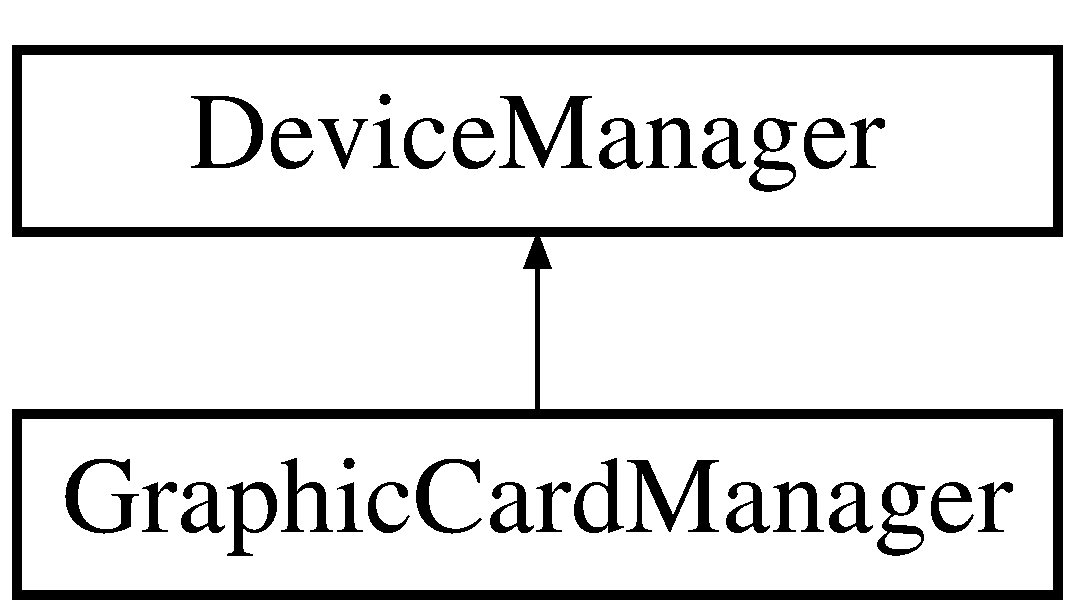
\includegraphics[height=2.000000cm]{classGraphicCardManager}
\end{center}
\end{figure}
\subsection*{Public Member Functions}
\begin{DoxyCompactItemize}
\item 
void \hyperlink{classGraphicCardManager_a6c94b17b01bd0f27bf0822c269d1c41c}{generate\+All\+Devices} ()
\item 
\hyperlink{classHWDevice}{H\+W\+Device} $\ast$ \hyperlink{classGraphicCardManager_a1835a9054bccb574e74dc2ebb2c28554}{generate\+New\+Device} (int position)
\item 
void \hyperlink{classGraphicCardManager_a42bc616062f94b2e4ee92a79ba537a16}{set\+Commands} (int device\+Position)
\item 
\hyperlink{classBaseDifference}{Base\+Difference} $\ast$$\ast$ \hyperlink{classGraphicCardManager_a17d988dac37f04cb1dddd45eef8c3aea}{generate\+Log\+Difference} ()
\item 
\hyperlink{classHWDevice}{H\+W\+Device} $\ast$ \hyperlink{classGraphicCardManager_ac71590c819520e60a491c8e69252efe1}{generate\+Fake\+Device} ()
\end{DoxyCompactItemize}
\subsection*{Additional Inherited Members}


\subsection{Member Function Documentation}
\index{Graphic\+Card\+Manager@{Graphic\+Card\+Manager}!generate\+All\+Devices@{generate\+All\+Devices}}
\index{generate\+All\+Devices@{generate\+All\+Devices}!Graphic\+Card\+Manager@{Graphic\+Card\+Manager}}
\subsubsection[{\texorpdfstring{generate\+All\+Devices()}{generateAllDevices()}}]{\setlength{\rightskip}{0pt plus 5cm}void Graphic\+Card\+Manager\+::generate\+All\+Devices (
\begin{DoxyParamCaption}
{}
\end{DoxyParamCaption}
)\hspace{0.3cm}{\ttfamily [virtual]}}\hypertarget{classGraphicCardManager_a6c94b17b01bd0f27bf0822c269d1c41c}{}\label{classGraphicCardManager_a6c94b17b01bd0f27bf0822c269d1c41c}
Generate and populate the devices array. This method will be overwritten from the specific classes (\hyperlink{classBIOS}{B\+I\+OS}, H\+DD, ecc..) 

Implements \hyperlink{classDeviceManager_ae9fa3bd3aa66f373d7748628b7ba26cc}{Device\+Manager}.

\index{Graphic\+Card\+Manager@{Graphic\+Card\+Manager}!generate\+Fake\+Device@{generate\+Fake\+Device}}
\index{generate\+Fake\+Device@{generate\+Fake\+Device}!Graphic\+Card\+Manager@{Graphic\+Card\+Manager}}
\subsubsection[{\texorpdfstring{generate\+Fake\+Device()}{generateFakeDevice()}}]{\setlength{\rightskip}{0pt plus 5cm}{\bf H\+W\+Device} $\ast$ Graphic\+Card\+Manager\+::generate\+Fake\+Device (
\begin{DoxyParamCaption}
{}
\end{DoxyParamCaption}
)\hspace{0.3cm}{\ttfamily [virtual]}}\hypertarget{classGraphicCardManager_ac71590c819520e60a491c8e69252efe1}{}\label{classGraphicCardManager_ac71590c819520e60a491c8e69252efe1}
This abstract method will produce a Fake (Specified by the concrete classes) Device that will be used later to compare devices 

Implements \hyperlink{classDeviceManager_a218031345b7b61c79f427985d950c3f3}{Device\+Manager}.

\index{Graphic\+Card\+Manager@{Graphic\+Card\+Manager}!generate\+Log\+Difference@{generate\+Log\+Difference}}
\index{generate\+Log\+Difference@{generate\+Log\+Difference}!Graphic\+Card\+Manager@{Graphic\+Card\+Manager}}
\subsubsection[{\texorpdfstring{generate\+Log\+Difference()}{generateLogDifference()}}]{\setlength{\rightskip}{0pt plus 5cm}{\bf Base\+Difference} $\ast$$\ast$ Graphic\+Card\+Manager\+::generate\+Log\+Difference (
\begin{DoxyParamCaption}
{}
\end{DoxyParamCaption}
)\hspace{0.3cm}{\ttfamily [virtual]}}\hypertarget{classGraphicCardManager_a17d988dac37f04cb1dddd45eef8c3aea}{}\label{classGraphicCardManager_a17d988dac37f04cb1dddd45eef8c3aea}
This abstract method will produce a \hyperlink{classBaseDifference}{Base\+Difference}, it will be used to compare different  between them.

\begin{DoxyReturn}{Returns}
the differences to populate 
\end{DoxyReturn}


Implements \hyperlink{classDeviceManager_ae9916011e50a6a48aea3d87b6c44b27e}{Device\+Manager}.

\index{Graphic\+Card\+Manager@{Graphic\+Card\+Manager}!generate\+New\+Device@{generate\+New\+Device}}
\index{generate\+New\+Device@{generate\+New\+Device}!Graphic\+Card\+Manager@{Graphic\+Card\+Manager}}
\subsubsection[{\texorpdfstring{generate\+New\+Device(int position)}{generateNewDevice(int position)}}]{\setlength{\rightskip}{0pt plus 5cm}{\bf H\+W\+Device} $\ast$ Graphic\+Card\+Manager\+::generate\+New\+Device (
\begin{DoxyParamCaption}
\item[{int}]{position}
\end{DoxyParamCaption}
)\hspace{0.3cm}{\ttfamily [virtual]}}\hypertarget{classGraphicCardManager_a1835a9054bccb574e74dc2ebb2c28554}{}\label{classGraphicCardManager_a1835a9054bccb574e74dc2ebb2c28554}
Generate and return a new device in a specific position.


\begin{DoxyParams}{Parameters}
{\em position} & used by the device \\
\hline
\end{DoxyParams}
\begin{DoxyReturn}{Returns}
the generated device 
\end{DoxyReturn}


Implements \hyperlink{classDeviceManager_a64c7c17d8cb8d407361dbcf8f6f17ccf}{Device\+Manager}.

\index{Graphic\+Card\+Manager@{Graphic\+Card\+Manager}!set\+Commands@{set\+Commands}}
\index{set\+Commands@{set\+Commands}!Graphic\+Card\+Manager@{Graphic\+Card\+Manager}}
\subsubsection[{\texorpdfstring{set\+Commands(int device\+Position)}{setCommands(int devicePosition)}}]{\setlength{\rightskip}{0pt plus 5cm}void Graphic\+Card\+Manager\+::set\+Commands (
\begin{DoxyParamCaption}
\item[{int}]{device\+Position}
\end{DoxyParamCaption}
)\hspace{0.3cm}{\ttfamily [virtual]}}\hypertarget{classGraphicCardManager_a42bc616062f94b2e4ee92a79ba537a16}{}\label{classGraphicCardManager_a42bc616062f94b2e4ee92a79ba537a16}
Set all commands used to retrieve infos. This method will be overwritten from the specific classes (\hyperlink{classBIOS}{B\+I\+OS}, H\+DD, ecc...)


\begin{DoxyParams}{Parameters}
{\em device\+Position} & the device position in the devices array \\
\hline
\end{DoxyParams}


Implements \hyperlink{classDeviceManager_ae367c6847b2988cf6249cbf6254261cb}{Device\+Manager}.



The documentation for this class was generated from the following files\+:\begin{DoxyCompactItemize}
\item 
/home/doomdiskday/workspace2/main/src/model/\+H\+W/\+Graphic\+Card/Graphic\+Card\+Manager.\+h\item 
/home/doomdiskday/workspace2/main/src/model/\+H\+W/\+Graphic\+Card/Graphic\+Card\+Manager.\+cpp\end{DoxyCompactItemize}

\hypertarget{classHardDisk}{}\section{Hard\+Disk Class Reference}
\label{classHardDisk}\index{Hard\+Disk@{Hard\+Disk}}
Inheritance diagram for Hard\+Disk\+:\begin{figure}[H]
\begin{center}
\leavevmode
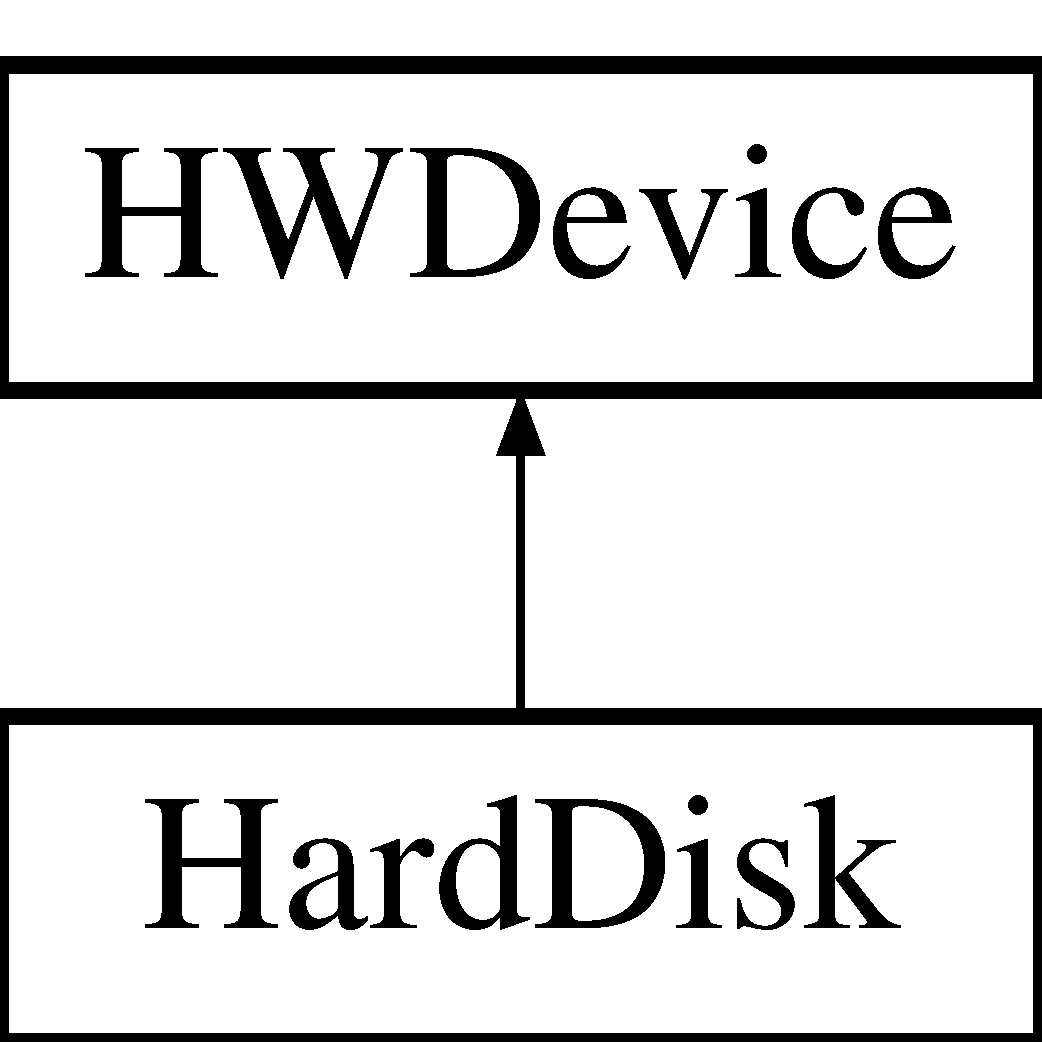
\includegraphics[height=2.000000cm]{classHardDisk}
\end{center}
\end{figure}
\subsection*{Public Member Functions}
\begin{DoxyCompactItemize}
\item 
{\bfseries Hard\+Disk} (int position)\hypertarget{classHardDisk_a48f797f4d6e17eb804ce29a3910fda85}{}\label{classHardDisk_a48f797f4d6e17eb804ce29a3910fda85}

\end{DoxyCompactItemize}
\subsection*{Additional Inherited Members}


The documentation for this class was generated from the following file\+:\begin{DoxyCompactItemize}
\item 
/home/doomdiskday/workspace2/main/src/model/\+H\+W/\+H\+D\+D/Hard\+Disk.\+h\end{DoxyCompactItemize}

\hypertarget{classHardDiskManager}{}\section{Hard\+Disk\+Manager Class Reference}
\label{classHardDiskManager}\index{Hard\+Disk\+Manager@{Hard\+Disk\+Manager}}
Inheritance diagram for Hard\+Disk\+Manager\+:\begin{figure}[H]
\begin{center}
\leavevmode
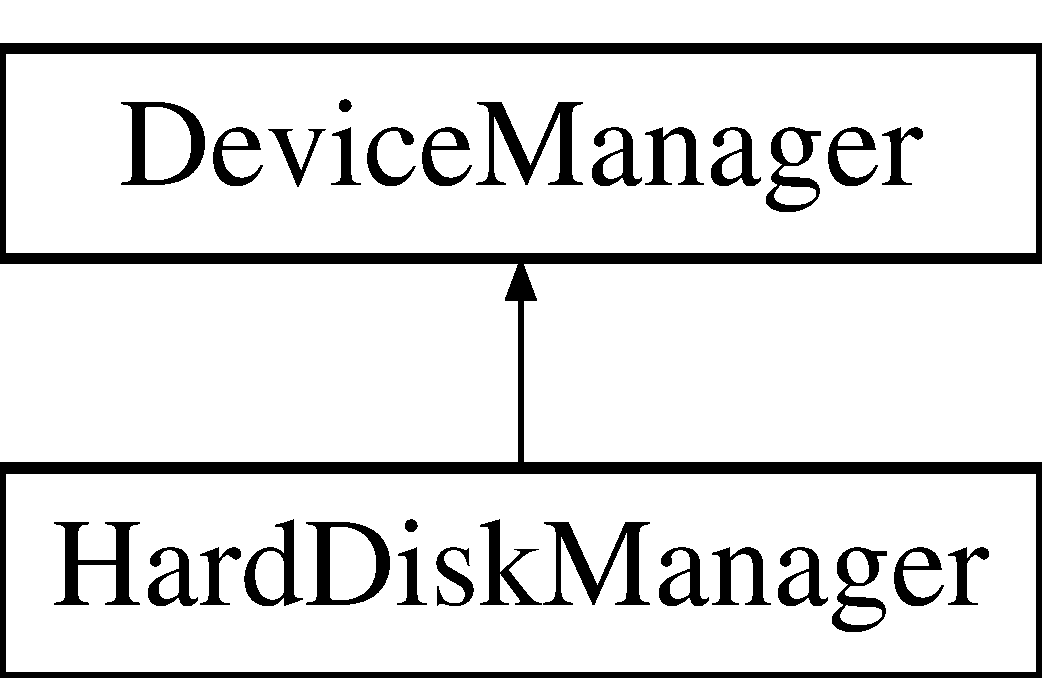
\includegraphics[height=2.000000cm]{classHardDiskManager}
\end{center}
\end{figure}
\subsection*{Public Member Functions}
\begin{DoxyCompactItemize}
\item 
void \hyperlink{classHardDiskManager_ac69f4cfc902fa23ff238f33ee9731c3c}{generate\+All\+Devices} ()
\item 
\hyperlink{classHWDevice}{H\+W\+Device} $\ast$ \hyperlink{classHardDiskManager_a3960650a3232567f3488fb10fb10fa7c}{generate\+New\+Device} (int position)
\item 
void \hyperlink{classHardDiskManager_a8e219e6e508dd2d8a6190c44bcf45782}{set\+Commands} (int device\+Position)
\item 
\hyperlink{classBaseDifference}{Base\+Difference} $\ast$$\ast$ \hyperlink{classHardDiskManager_ae8579afefc3c0619ef05c30b9fda3b82}{generate\+Log\+Difference} ()
\item 
\hyperlink{classHWDevice}{H\+W\+Device} $\ast$ \hyperlink{classHardDiskManager_a586e786b4512ec8dfb79edb743794b77}{generate\+Fake\+Device} ()
\end{DoxyCompactItemize}
\subsection*{Additional Inherited Members}


\subsection{Member Function Documentation}
\index{Hard\+Disk\+Manager@{Hard\+Disk\+Manager}!generate\+All\+Devices@{generate\+All\+Devices}}
\index{generate\+All\+Devices@{generate\+All\+Devices}!Hard\+Disk\+Manager@{Hard\+Disk\+Manager}}
\subsubsection[{\texorpdfstring{generate\+All\+Devices()}{generateAllDevices()}}]{\setlength{\rightskip}{0pt plus 5cm}void Hard\+Disk\+Manager\+::generate\+All\+Devices (
\begin{DoxyParamCaption}
{}
\end{DoxyParamCaption}
)\hspace{0.3cm}{\ttfamily [virtual]}}\hypertarget{classHardDiskManager_ac69f4cfc902fa23ff238f33ee9731c3c}{}\label{classHardDiskManager_ac69f4cfc902fa23ff238f33ee9731c3c}
Generate and populate the devices array. This method will be overwritten from the specific classes (\hyperlink{classBIOS}{B\+I\+OS}, H\+DD, ecc..) 

Implements \hyperlink{classDeviceManager_ae9fa3bd3aa66f373d7748628b7ba26cc}{Device\+Manager}.

\index{Hard\+Disk\+Manager@{Hard\+Disk\+Manager}!generate\+Fake\+Device@{generate\+Fake\+Device}}
\index{generate\+Fake\+Device@{generate\+Fake\+Device}!Hard\+Disk\+Manager@{Hard\+Disk\+Manager}}
\subsubsection[{\texorpdfstring{generate\+Fake\+Device()}{generateFakeDevice()}}]{\setlength{\rightskip}{0pt plus 5cm}{\bf H\+W\+Device} $\ast$ Hard\+Disk\+Manager\+::generate\+Fake\+Device (
\begin{DoxyParamCaption}
{}
\end{DoxyParamCaption}
)\hspace{0.3cm}{\ttfamily [virtual]}}\hypertarget{classHardDiskManager_a586e786b4512ec8dfb79edb743794b77}{}\label{classHardDiskManager_a586e786b4512ec8dfb79edb743794b77}
This abstract method will produce a Fake (Specified by the concrete classes) Device that will be used later to compare devices 

Implements \hyperlink{classDeviceManager_a218031345b7b61c79f427985d950c3f3}{Device\+Manager}.

\index{Hard\+Disk\+Manager@{Hard\+Disk\+Manager}!generate\+Log\+Difference@{generate\+Log\+Difference}}
\index{generate\+Log\+Difference@{generate\+Log\+Difference}!Hard\+Disk\+Manager@{Hard\+Disk\+Manager}}
\subsubsection[{\texorpdfstring{generate\+Log\+Difference()}{generateLogDifference()}}]{\setlength{\rightskip}{0pt plus 5cm}{\bf Base\+Difference} $\ast$$\ast$ Hard\+Disk\+Manager\+::generate\+Log\+Difference (
\begin{DoxyParamCaption}
{}
\end{DoxyParamCaption}
)\hspace{0.3cm}{\ttfamily [virtual]}}\hypertarget{classHardDiskManager_ae8579afefc3c0619ef05c30b9fda3b82}{}\label{classHardDiskManager_ae8579afefc3c0619ef05c30b9fda3b82}
This abstract method will produce a \hyperlink{classBaseDifference}{Base\+Difference}, it will be used to compare different  between them.

\begin{DoxyReturn}{Returns}
the differences to populate 
\end{DoxyReturn}


Implements \hyperlink{classDeviceManager_ae9916011e50a6a48aea3d87b6c44b27e}{Device\+Manager}.

\index{Hard\+Disk\+Manager@{Hard\+Disk\+Manager}!generate\+New\+Device@{generate\+New\+Device}}
\index{generate\+New\+Device@{generate\+New\+Device}!Hard\+Disk\+Manager@{Hard\+Disk\+Manager}}
\subsubsection[{\texorpdfstring{generate\+New\+Device(int position)}{generateNewDevice(int position)}}]{\setlength{\rightskip}{0pt plus 5cm}{\bf H\+W\+Device} $\ast$ Hard\+Disk\+Manager\+::generate\+New\+Device (
\begin{DoxyParamCaption}
\item[{int}]{position}
\end{DoxyParamCaption}
)\hspace{0.3cm}{\ttfamily [virtual]}}\hypertarget{classHardDiskManager_a3960650a3232567f3488fb10fb10fa7c}{}\label{classHardDiskManager_a3960650a3232567f3488fb10fb10fa7c}
Generate and return a new device in a specific position.


\begin{DoxyParams}{Parameters}
{\em position} & used by the device \\
\hline
\end{DoxyParams}
\begin{DoxyReturn}{Returns}
the generated device 
\end{DoxyReturn}


Implements \hyperlink{classDeviceManager_a64c7c17d8cb8d407361dbcf8f6f17ccf}{Device\+Manager}.

\index{Hard\+Disk\+Manager@{Hard\+Disk\+Manager}!set\+Commands@{set\+Commands}}
\index{set\+Commands@{set\+Commands}!Hard\+Disk\+Manager@{Hard\+Disk\+Manager}}
\subsubsection[{\texorpdfstring{set\+Commands(int device\+Position)}{setCommands(int devicePosition)}}]{\setlength{\rightskip}{0pt plus 5cm}void Hard\+Disk\+Manager\+::set\+Commands (
\begin{DoxyParamCaption}
\item[{int}]{device\+Position}
\end{DoxyParamCaption}
)\hspace{0.3cm}{\ttfamily [virtual]}}\hypertarget{classHardDiskManager_a8e219e6e508dd2d8a6190c44bcf45782}{}\label{classHardDiskManager_a8e219e6e508dd2d8a6190c44bcf45782}
Set all commands used to retrieve infos. This method will be overwritten from the specific classes (\hyperlink{classBIOS}{B\+I\+OS}, H\+DD, ecc...)


\begin{DoxyParams}{Parameters}
{\em device\+Position} & the device position in the devices array \\
\hline
\end{DoxyParams}


Implements \hyperlink{classDeviceManager_ae367c6847b2988cf6249cbf6254261cb}{Device\+Manager}.



The documentation for this class was generated from the following files\+:\begin{DoxyCompactItemize}
\item 
/home/doomdiskday/workspace2/main/src/model/\+H\+W/\+H\+D\+D/Hard\+Disk\+Manager.\+h\item 
/home/doomdiskday/workspace2/main/src/model/\+H\+W/\+H\+D\+D/Hard\+Disk\+Manager.\+cpp\end{DoxyCompactItemize}

\hypertarget{classhelper__cmdManager}{}\section{helper\+\_\+cmd\+Manager Class Reference}
\label{classhelper__cmdManager}\index{helper\+\_\+cmd\+Manager@{helper\+\_\+cmd\+Manager}}


{\ttfamily \#include $<$Command\+Manager.\+h$>$}

Inheritance diagram for helper\+\_\+cmd\+Manager\+:\begin{figure}[H]
\begin{center}
\leavevmode
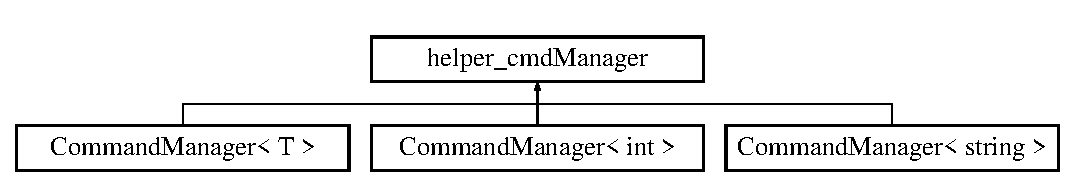
\includegraphics[height=2.000000cm]{classhelper__cmdManager}
\end{center}
\end{figure}
\subsection*{Public Member Functions}
\begin{DoxyCompactItemize}
\item 
string \hyperlink{classhelper__cmdManager_a38b9a436b41fb2774fb3201b9248caef}{Get\+Stdout\+From\+Command} (\hyperlink{classCommand}{Command} $\ast$cmd)
\end{DoxyCompactItemize}


\subsection{Detailed Description}
This helper contains all common methods for differents command\+Managers 

\subsection{Member Function Documentation}
\index{helper\+\_\+cmd\+Manager@{helper\+\_\+cmd\+Manager}!Get\+Stdout\+From\+Command@{Get\+Stdout\+From\+Command}}
\index{Get\+Stdout\+From\+Command@{Get\+Stdout\+From\+Command}!helper\+\_\+cmd\+Manager@{helper\+\_\+cmd\+Manager}}
\subsubsection[{\texorpdfstring{Get\+Stdout\+From\+Command(\+Command $\ast$cmd)}{GetStdoutFromCommand(Command *cmd)}}]{\setlength{\rightskip}{0pt plus 5cm}string helper\+\_\+cmd\+Manager\+::\+Get\+Stdout\+From\+Command (
\begin{DoxyParamCaption}
\item[{{\bf Command} $\ast$}]{cmd}
\end{DoxyParamCaption}
)\hspace{0.3cm}{\ttfamily [inline]}}\hypertarget{classhelper__cmdManager_a38b9a436b41fb2774fb3201b9248caef}{}\label{classhelper__cmdManager_a38b9a436b41fb2774fb3201b9248caef}
execute a command and return the stdout


\begin{DoxyParams}{Parameters}
{\em cmd} & the command to execute \\
\hline
\end{DoxyParams}


The documentation for this class was generated from the following file\+:\begin{DoxyCompactItemize}
\item 
/home/doomdiskday/workspace2/main/src/utils/Command\+Manager.\+h\end{DoxyCompactItemize}

\hypertarget{classHWDevice}{}\section{H\+W\+Device Class Reference}
\label{classHWDevice}\index{H\+W\+Device@{H\+W\+Device}}


{\ttfamily \#include $<$H\+W\+Device.\+h$>$}

Inheritance diagram for H\+W\+Device\+:\begin{figure}[H]
\begin{center}
\leavevmode
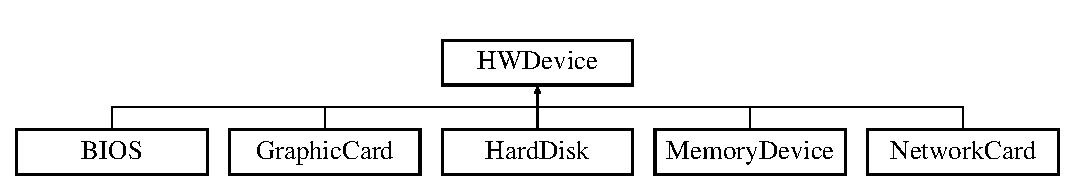
\includegraphics[height=2.000000cm]{classHWDevice}
\end{center}
\end{figure}
\subsection*{Public Member Functions}
\begin{DoxyCompactItemize}
\item 
\hyperlink{classBaseProperty}{Base\+Property} $\ast$ \hyperlink{classHWDevice_a657e562484d584cd3c1d2c9938b4865c}{get\+Property} (int property\+Position)
\end{DoxyCompactItemize}
\subsection*{Protected Attributes}
\begin{DoxyCompactItemize}
\item 
\hyperlink{classBaseProperty}{Base\+Property} $\ast$$\ast$ {\bfseries device\+Infos}\hypertarget{classHWDevice_a6987786c30ac6a7c026e2dc099a7a124}{}\label{classHWDevice_a6987786c30ac6a7c026e2dc099a7a124}

\end{DoxyCompactItemize}


\subsection{Detailed Description}
This class represents an Hardware Device 

\subsection{Member Function Documentation}
\index{H\+W\+Device@{H\+W\+Device}!get\+Property@{get\+Property}}
\index{get\+Property@{get\+Property}!H\+W\+Device@{H\+W\+Device}}
\subsubsection[{\texorpdfstring{get\+Property(int property\+Position)}{getProperty(int propertyPosition)}}]{\setlength{\rightskip}{0pt plus 5cm}{\bf Base\+Property}$\ast$ H\+W\+Device\+::get\+Property (
\begin{DoxyParamCaption}
\item[{int}]{property\+Position}
\end{DoxyParamCaption}
)\hspace{0.3cm}{\ttfamily [inline]}}\hypertarget{classHWDevice_a657e562484d584cd3c1d2c9938b4865c}{}\label{classHWDevice_a657e562484d584cd3c1d2c9938b4865c}
Return a specific property


\begin{DoxyParams}{Parameters}
{\em property\+Position} & the property position \\
\hline
\end{DoxyParams}
\begin{DoxyReturn}{Returns}
a specific property 
\end{DoxyReturn}


The documentation for this class was generated from the following file\+:\begin{DoxyCompactItemize}
\item 
/home/doomdiskday/workspace2/main/src/model/\+H\+W/\+Basic/H\+W\+Device.\+h\end{DoxyCompactItemize}

\hypertarget{classHWManager}{}\section{H\+W\+Manager Class Reference}
\label{classHWManager}\index{H\+W\+Manager@{H\+W\+Manager}}
\subsection*{Public Member Functions}
\begin{DoxyCompactItemize}
\item 
void \hyperlink{classHWManager_a867e8247ccb2c2853cde8d4461aa5b7d}{populate\+Manager} (check\+Choise choise)
\item 
void \hyperlink{classHWManager_aeec8928295c6658cfbd3b292872d8f41}{populate\+All\+Managers} ()
\item 
void \hyperlink{classHWManager_a1b94c4885dc128d740686b5bb96caec8}{populate\+Devices} (check\+Choise choise)
\item 
void \hyperlink{classHWManager_a91d0c86ad3344faf5cac802ea3f38516}{populate\+All\+Devices} ()
\item 
int \hyperlink{classHWManager_aea84312971b2f37424ac48b98ec6aeca}{get\+Number\+Of\+Devices} ()
\item 
void \hyperlink{classHWManager_a19ca6cfbb5d1e7f83a14a6a35b1fa303}{generate\+Log\+Dir} ()
\item 
void \hyperlink{classHWManager_a17459fb942af258ec4ac39d34c70bad8}{generate\+All\+Logs} ()
\item 
void \hyperlink{classHWManager_a9bd4de108a88b3554526e50fe67b3e71}{retrieve\+Devices\+From\+File} (string path)
\item 
void \hyperlink{classHWManager_a95a7659252ca203578a74ec393ad94f7}{print\+All\+Infos} ()
\item 
void \hyperlink{classHWManager_a1fe7d46d9978b65ffb1d29de7cc4a93c}{check\+With\+Default\+Directory} ()
\item 
void \hyperlink{classHWManager_a175ba9eab5c1f149aafc491636f36390}{check\+With\+File} (string path, check\+Choise choise)
\end{DoxyCompactItemize}


\subsection{Member Function Documentation}
\index{H\+W\+Manager@{H\+W\+Manager}!check\+With\+Default\+Directory@{check\+With\+Default\+Directory}}
\index{check\+With\+Default\+Directory@{check\+With\+Default\+Directory}!H\+W\+Manager@{H\+W\+Manager}}
\subsubsection[{\texorpdfstring{check\+With\+Default\+Directory()}{checkWithDefaultDirectory()}}]{\setlength{\rightskip}{0pt plus 5cm}void H\+W\+Manager\+::check\+With\+Default\+Directory (
\begin{DoxyParamCaption}
{}
\end{DoxyParamCaption}
)}\hypertarget{classHWManager_a1fe7d46d9978b65ffb1d29de7cc4a93c}{}\label{classHWManager_a1fe7d46d9978b65ffb1d29de7cc4a93c}
This method check current devices with devices stored in default log directory \index{H\+W\+Manager@{H\+W\+Manager}!check\+With\+File@{check\+With\+File}}
\index{check\+With\+File@{check\+With\+File}!H\+W\+Manager@{H\+W\+Manager}}
\subsubsection[{\texorpdfstring{check\+With\+File(string path, check\+Choise choise)}{checkWithFile(string path, checkChoise choise)}}]{\setlength{\rightskip}{0pt plus 5cm}void H\+W\+Manager\+::check\+With\+File (
\begin{DoxyParamCaption}
\item[{string}]{path, }
\item[{check\+Choise}]{choise}
\end{DoxyParamCaption}
)}\hypertarget{classHWManager_a175ba9eab5c1f149aafc491636f36390}{}\label{classHWManager_a175ba9eab5c1f149aafc491636f36390}
This method check current devices with devices stored in a log file passed by param


\begin{DoxyParams}{Parameters}
{\em path} & the log file path  the devicemanager choise \\
\hline
\end{DoxyParams}
\index{H\+W\+Manager@{H\+W\+Manager}!generate\+All\+Logs@{generate\+All\+Logs}}
\index{generate\+All\+Logs@{generate\+All\+Logs}!H\+W\+Manager@{H\+W\+Manager}}
\subsubsection[{\texorpdfstring{generate\+All\+Logs()}{generateAllLogs()}}]{\setlength{\rightskip}{0pt plus 5cm}void H\+W\+Manager\+::generate\+All\+Logs (
\begin{DoxyParamCaption}
{}
\end{DoxyParamCaption}
)}\hypertarget{classHWManager_a17459fb942af258ec4ac39d34c70bad8}{}\label{classHWManager_a17459fb942af258ec4ac39d34c70bad8}
This method generate all logs from the device managers \index{H\+W\+Manager@{H\+W\+Manager}!generate\+Log\+Dir@{generate\+Log\+Dir}}
\index{generate\+Log\+Dir@{generate\+Log\+Dir}!H\+W\+Manager@{H\+W\+Manager}}
\subsubsection[{\texorpdfstring{generate\+Log\+Dir()}{generateLogDir()}}]{\setlength{\rightskip}{0pt plus 5cm}void H\+W\+Manager\+::generate\+Log\+Dir (
\begin{DoxyParamCaption}
{}
\end{DoxyParamCaption}
)}\hypertarget{classHWManager_a19ca6cfbb5d1e7f83a14a6a35b1fa303}{}\label{classHWManager_a19ca6cfbb5d1e7f83a14a6a35b1fa303}
This method generate the main log directory \index{H\+W\+Manager@{H\+W\+Manager}!get\+Number\+Of\+Devices@{get\+Number\+Of\+Devices}}
\index{get\+Number\+Of\+Devices@{get\+Number\+Of\+Devices}!H\+W\+Manager@{H\+W\+Manager}}
\subsubsection[{\texorpdfstring{get\+Number\+Of\+Devices()}{getNumberOfDevices()}}]{\setlength{\rightskip}{0pt plus 5cm}int H\+W\+Manager\+::get\+Number\+Of\+Devices (
\begin{DoxyParamCaption}
{}
\end{DoxyParamCaption}
)}\hypertarget{classHWManager_aea84312971b2f37424ac48b98ec6aeca}{}\label{classHWManager_aea84312971b2f37424ac48b98ec6aeca}
This method return the number of devices retrieved on the system \index{H\+W\+Manager@{H\+W\+Manager}!populate\+All\+Devices@{populate\+All\+Devices}}
\index{populate\+All\+Devices@{populate\+All\+Devices}!H\+W\+Manager@{H\+W\+Manager}}
\subsubsection[{\texorpdfstring{populate\+All\+Devices()}{populateAllDevices()}}]{\setlength{\rightskip}{0pt plus 5cm}void H\+W\+Manager\+::populate\+All\+Devices (
\begin{DoxyParamCaption}
{}
\end{DoxyParamCaption}
)}\hypertarget{classHWManager_a91d0c86ad3344faf5cac802ea3f38516}{}\label{classHWManager_a91d0c86ad3344faf5cac802ea3f38516}
This method populate all manager\textquotesingle{}s devices \index{H\+W\+Manager@{H\+W\+Manager}!populate\+All\+Managers@{populate\+All\+Managers}}
\index{populate\+All\+Managers@{populate\+All\+Managers}!H\+W\+Manager@{H\+W\+Manager}}
\subsubsection[{\texorpdfstring{populate\+All\+Managers()}{populateAllManagers()}}]{\setlength{\rightskip}{0pt plus 5cm}void H\+W\+Manager\+::populate\+All\+Managers (
\begin{DoxyParamCaption}
{}
\end{DoxyParamCaption}
)}\hypertarget{classHWManager_aeec8928295c6658cfbd3b292872d8f41}{}\label{classHWManager_aeec8928295c6658cfbd3b292872d8f41}
This method populate all managers \index{H\+W\+Manager@{H\+W\+Manager}!populate\+Devices@{populate\+Devices}}
\index{populate\+Devices@{populate\+Devices}!H\+W\+Manager@{H\+W\+Manager}}
\subsubsection[{\texorpdfstring{populate\+Devices(check\+Choise choise)}{populateDevices(checkChoise choise)}}]{\setlength{\rightskip}{0pt plus 5cm}void H\+W\+Manager\+::populate\+Devices (
\begin{DoxyParamCaption}
\item[{check\+Choise}]{choise}
\end{DoxyParamCaption}
)}\hypertarget{classHWManager_a1b94c4885dc128d740686b5bb96caec8}{}\label{classHWManager_a1b94c4885dc128d740686b5bb96caec8}
This method populate a specific class of devices


\begin{DoxyParams}{Parameters}
{\em choise} & the class to populate \\
\hline
\end{DoxyParams}
\index{H\+W\+Manager@{H\+W\+Manager}!populate\+Manager@{populate\+Manager}}
\index{populate\+Manager@{populate\+Manager}!H\+W\+Manager@{H\+W\+Manager}}
\subsubsection[{\texorpdfstring{populate\+Manager(check\+Choise choise)}{populateManager(checkChoise choise)}}]{\setlength{\rightskip}{0pt plus 5cm}void H\+W\+Manager\+::populate\+Manager (
\begin{DoxyParamCaption}
\item[{check\+Choise}]{choise}
\end{DoxyParamCaption}
)}\hypertarget{classHWManager_a867e8247ccb2c2853cde8d4461aa5b7d}{}\label{classHWManager_a867e8247ccb2c2853cde8d4461aa5b7d}
This method instantiate the choosed manager


\begin{DoxyParams}{Parameters}
{\em choise} & the user\textquotesingle{}s choice \\
\hline
\end{DoxyParams}
\index{H\+W\+Manager@{H\+W\+Manager}!print\+All\+Infos@{print\+All\+Infos}}
\index{print\+All\+Infos@{print\+All\+Infos}!H\+W\+Manager@{H\+W\+Manager}}
\subsubsection[{\texorpdfstring{print\+All\+Infos()}{printAllInfos()}}]{\setlength{\rightskip}{0pt plus 5cm}void H\+W\+Manager\+::print\+All\+Infos (
\begin{DoxyParamCaption}
{}
\end{DoxyParamCaption}
)}\hypertarget{classHWManager_a95a7659252ca203578a74ec393ad94f7}{}\label{classHWManager_a95a7659252ca203578a74ec393ad94f7}
This method print all infos about devices retrieved \index{H\+W\+Manager@{H\+W\+Manager}!retrieve\+Devices\+From\+File@{retrieve\+Devices\+From\+File}}
\index{retrieve\+Devices\+From\+File@{retrieve\+Devices\+From\+File}!H\+W\+Manager@{H\+W\+Manager}}
\subsubsection[{\texorpdfstring{retrieve\+Devices\+From\+File(string path)}{retrieveDevicesFromFile(string path)}}]{\setlength{\rightskip}{0pt plus 5cm}void H\+W\+Manager\+::retrieve\+Devices\+From\+File (
\begin{DoxyParamCaption}
\item[{string}]{path}
\end{DoxyParamCaption}
)}\hypertarget{classHWManager_a9bd4de108a88b3554526e50fe67b3e71}{}\label{classHWManager_a9bd4de108a88b3554526e50fe67b3e71}
This method show all devices logged in a file


\begin{DoxyParams}{Parameters}
{\em path} & path of log file \\
\hline
\end{DoxyParams}


The documentation for this class was generated from the following files\+:\begin{DoxyCompactItemize}
\item 
/home/doomdiskday/workspace2/main/src/model/\+H\+W/\+Manager/H\+W\+Manager.\+h\item 
/home/doomdiskday/workspace2/main/src/model/\+H\+W/\+Manager/H\+W\+Manager.\+cpp\end{DoxyCompactItemize}

\hypertarget{classMemoryDevice}{}\section{Memory\+Device Class Reference}
\label{classMemoryDevice}\index{Memory\+Device@{Memory\+Device}}


{\ttfamily \#include $<$Memory\+Device.\+h$>$}

Inheritance diagram for Memory\+Device\+:\begin{figure}[H]
\begin{center}
\leavevmode
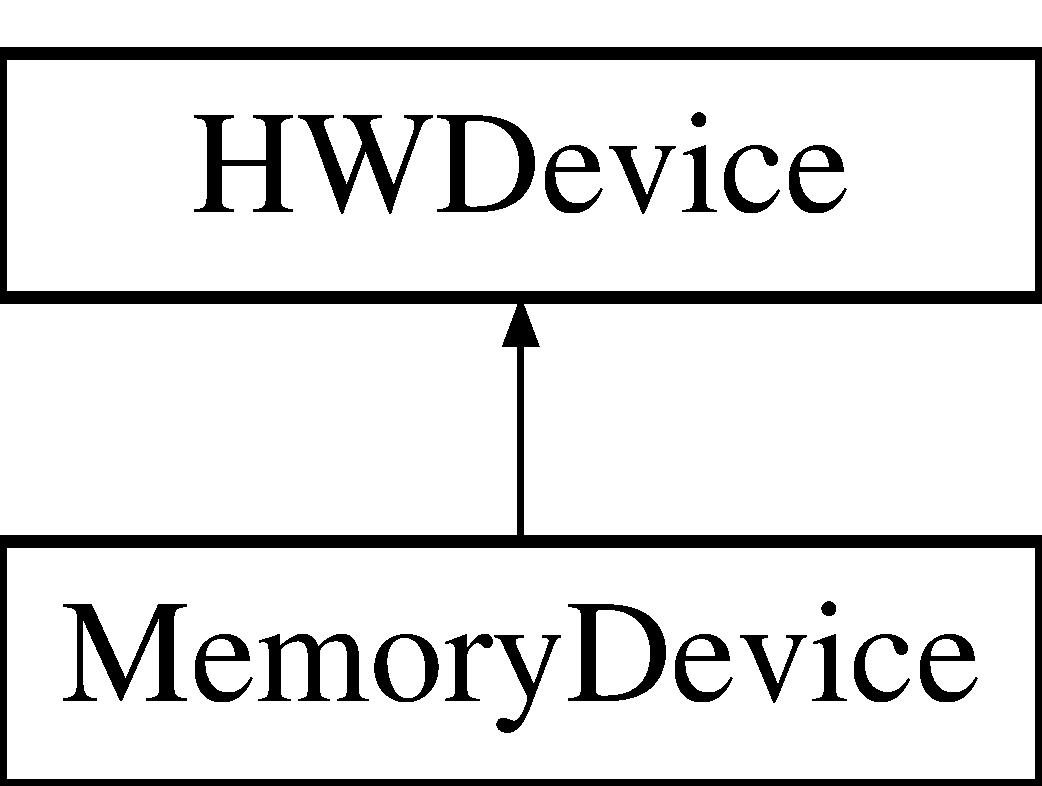
\includegraphics[height=2.000000cm]{classMemoryDevice}
\end{center}
\end{figure}
\subsection*{Public Member Functions}
\begin{DoxyCompactItemize}
\item 
{\bfseries Memory\+Device} (int position)\hypertarget{classMemoryDevice_a8f890a8d70b54abefa45ac1d6f7a28be}{}\label{classMemoryDevice_a8f890a8d70b54abefa45ac1d6f7a28be}

\end{DoxyCompactItemize}
\subsection*{Additional Inherited Members}


\subsection{Detailed Description}
This class represents a generic \hyperlink{classMemoryDevice}{Memory\+Device} 

The documentation for this class was generated from the following file\+:\begin{DoxyCompactItemize}
\item 
/home/doomdiskday/workspace2/main/src/model/\+H\+W/\+Memory/Memory\+Device.\+h\end{DoxyCompactItemize}

\hypertarget{classMemoryDeviceManager}{}\section{Memory\+Device\+Manager Class Reference}
\label{classMemoryDeviceManager}\index{Memory\+Device\+Manager@{Memory\+Device\+Manager}}


{\ttfamily \#include $<$Memory\+Device\+Manager.\+h$>$}

Inheritance diagram for Memory\+Device\+Manager\+:\begin{figure}[H]
\begin{center}
\leavevmode
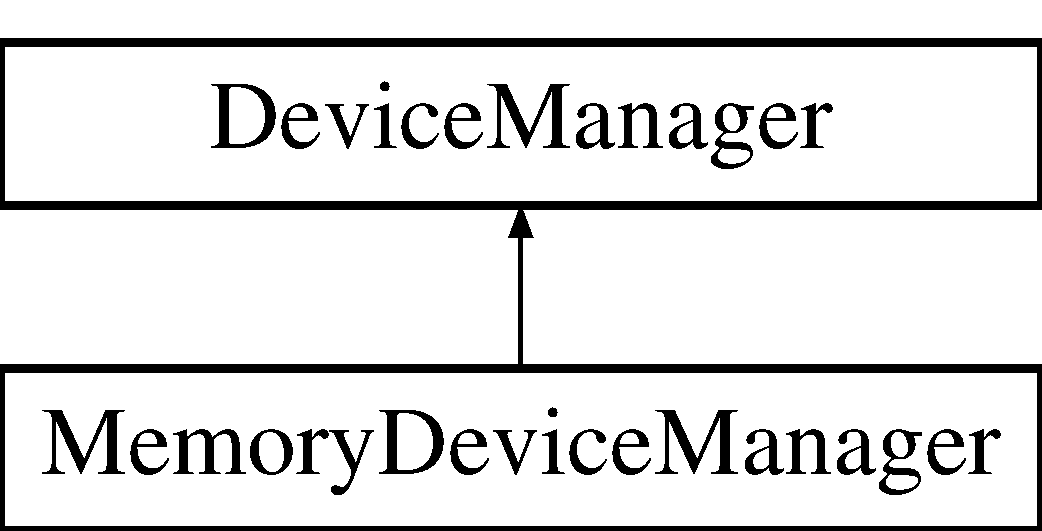
\includegraphics[height=2.000000cm]{classMemoryDeviceManager}
\end{center}
\end{figure}
\subsection*{Public Member Functions}
\begin{DoxyCompactItemize}
\item 
void \hyperlink{classMemoryDeviceManager_a84565386d5d9ada62c495558ba7c06f8}{generate\+All\+Devices} ()
\item 
\hyperlink{classHWDevice}{H\+W\+Device} $\ast$ \hyperlink{classMemoryDeviceManager_a2fa6b078f50c4bfbbbef218b8289ee89}{generate\+New\+Device} (int position)
\item 
void \hyperlink{classMemoryDeviceManager_a0246a46d583a717dfabc625a5e387400}{set\+Commands} (int device\+Position)
\item 
\hyperlink{classBaseDifference}{Base\+Difference} $\ast$$\ast$ \hyperlink{classMemoryDeviceManager_a1462e426adfe44f815359fb7f8b096b1}{generate\+Log\+Difference} ()
\item 
\hyperlink{classHWDevice}{H\+W\+Device} $\ast$ \hyperlink{classMemoryDeviceManager_aa652b05bfea23ce4dbe562ed158fb165}{generate\+Fake\+Device} ()
\end{DoxyCompactItemize}
\subsection*{Additional Inherited Members}


\subsection{Detailed Description}
Reppresents a Memory device manager, it\textquotesingle{}s used to manage all memory devices . 

\subsection{Member Function Documentation}
\index{Memory\+Device\+Manager@{Memory\+Device\+Manager}!generate\+All\+Devices@{generate\+All\+Devices}}
\index{generate\+All\+Devices@{generate\+All\+Devices}!Memory\+Device\+Manager@{Memory\+Device\+Manager}}
\subsubsection[{\texorpdfstring{generate\+All\+Devices()}{generateAllDevices()}}]{\setlength{\rightskip}{0pt plus 5cm}void Memory\+Device\+Manager\+::generate\+All\+Devices (
\begin{DoxyParamCaption}
{}
\end{DoxyParamCaption}
)\hspace{0.3cm}{\ttfamily [virtual]}}\hypertarget{classMemoryDeviceManager_a84565386d5d9ada62c495558ba7c06f8}{}\label{classMemoryDeviceManager_a84565386d5d9ada62c495558ba7c06f8}
Generate and populate the devices array. This method will be overwritten from the specific classes (\hyperlink{classBIOS}{B\+I\+OS}, H\+DD, ecc..) 

Implements \hyperlink{classDeviceManager_ae9fa3bd3aa66f373d7748628b7ba26cc}{Device\+Manager}.

\index{Memory\+Device\+Manager@{Memory\+Device\+Manager}!generate\+Fake\+Device@{generate\+Fake\+Device}}
\index{generate\+Fake\+Device@{generate\+Fake\+Device}!Memory\+Device\+Manager@{Memory\+Device\+Manager}}
\subsubsection[{\texorpdfstring{generate\+Fake\+Device()}{generateFakeDevice()}}]{\setlength{\rightskip}{0pt plus 5cm}{\bf H\+W\+Device} $\ast$ Memory\+Device\+Manager\+::generate\+Fake\+Device (
\begin{DoxyParamCaption}
{}
\end{DoxyParamCaption}
)\hspace{0.3cm}{\ttfamily [virtual]}}\hypertarget{classMemoryDeviceManager_aa652b05bfea23ce4dbe562ed158fb165}{}\label{classMemoryDeviceManager_aa652b05bfea23ce4dbe562ed158fb165}
This abstract method will produce a Fake (Specified by the concrete classes) Device that will be used later to compare devices 

Implements \hyperlink{classDeviceManager_a218031345b7b61c79f427985d950c3f3}{Device\+Manager}.

\index{Memory\+Device\+Manager@{Memory\+Device\+Manager}!generate\+Log\+Difference@{generate\+Log\+Difference}}
\index{generate\+Log\+Difference@{generate\+Log\+Difference}!Memory\+Device\+Manager@{Memory\+Device\+Manager}}
\subsubsection[{\texorpdfstring{generate\+Log\+Difference()}{generateLogDifference()}}]{\setlength{\rightskip}{0pt plus 5cm}{\bf Base\+Difference} $\ast$$\ast$ Memory\+Device\+Manager\+::generate\+Log\+Difference (
\begin{DoxyParamCaption}
{}
\end{DoxyParamCaption}
)\hspace{0.3cm}{\ttfamily [virtual]}}\hypertarget{classMemoryDeviceManager_a1462e426adfe44f815359fb7f8b096b1}{}\label{classMemoryDeviceManager_a1462e426adfe44f815359fb7f8b096b1}
This abstract method will produce a \hyperlink{classBaseDifference}{Base\+Difference}, it will be used to compare different  between them.

\begin{DoxyReturn}{Returns}
the differences to populate 
\end{DoxyReturn}


Implements \hyperlink{classDeviceManager_ae9916011e50a6a48aea3d87b6c44b27e}{Device\+Manager}.

\index{Memory\+Device\+Manager@{Memory\+Device\+Manager}!generate\+New\+Device@{generate\+New\+Device}}
\index{generate\+New\+Device@{generate\+New\+Device}!Memory\+Device\+Manager@{Memory\+Device\+Manager}}
\subsubsection[{\texorpdfstring{generate\+New\+Device(int position)}{generateNewDevice(int position)}}]{\setlength{\rightskip}{0pt plus 5cm}{\bf H\+W\+Device} $\ast$ Memory\+Device\+Manager\+::generate\+New\+Device (
\begin{DoxyParamCaption}
\item[{int}]{position}
\end{DoxyParamCaption}
)\hspace{0.3cm}{\ttfamily [virtual]}}\hypertarget{classMemoryDeviceManager_a2fa6b078f50c4bfbbbef218b8289ee89}{}\label{classMemoryDeviceManager_a2fa6b078f50c4bfbbbef218b8289ee89}
Generate and return a new device in a specific position.


\begin{DoxyParams}{Parameters}
{\em position} & used by the device \\
\hline
\end{DoxyParams}
\begin{DoxyReturn}{Returns}
the generated device 
\end{DoxyReturn}


Implements \hyperlink{classDeviceManager_a64c7c17d8cb8d407361dbcf8f6f17ccf}{Device\+Manager}.

\index{Memory\+Device\+Manager@{Memory\+Device\+Manager}!set\+Commands@{set\+Commands}}
\index{set\+Commands@{set\+Commands}!Memory\+Device\+Manager@{Memory\+Device\+Manager}}
\subsubsection[{\texorpdfstring{set\+Commands(int device\+Position)}{setCommands(int devicePosition)}}]{\setlength{\rightskip}{0pt plus 5cm}void Memory\+Device\+Manager\+::set\+Commands (
\begin{DoxyParamCaption}
\item[{int}]{device\+Position}
\end{DoxyParamCaption}
)\hspace{0.3cm}{\ttfamily [virtual]}}\hypertarget{classMemoryDeviceManager_a0246a46d583a717dfabc625a5e387400}{}\label{classMemoryDeviceManager_a0246a46d583a717dfabc625a5e387400}
Set all commands used to retrieve infos. This method will be overwritten from the specific classes (\hyperlink{classBIOS}{B\+I\+OS}, H\+DD, ecc...)


\begin{DoxyParams}{Parameters}
{\em device\+Position} & the device position in the devices array \\
\hline
\end{DoxyParams}


Implements \hyperlink{classDeviceManager_ae367c6847b2988cf6249cbf6254261cb}{Device\+Manager}.



The documentation for this class was generated from the following files\+:\begin{DoxyCompactItemize}
\item 
/home/doomdiskday/workspace2/main/src/model/\+H\+W/\+Memory/Memory\+Device\+Manager.\+h\item 
/home/doomdiskday/workspace2/main/src/model/\+H\+W/\+Memory/Memory\+Device\+Manager.\+cpp\end{DoxyCompactItemize}

\hypertarget{classNetworkCard}{}\section{Network\+Card Class Reference}
\label{classNetworkCard}\index{Network\+Card@{Network\+Card}}


{\ttfamily \#include $<$Network\+Card.\+h$>$}

Inheritance diagram for Network\+Card\+:\begin{figure}[H]
\begin{center}
\leavevmode
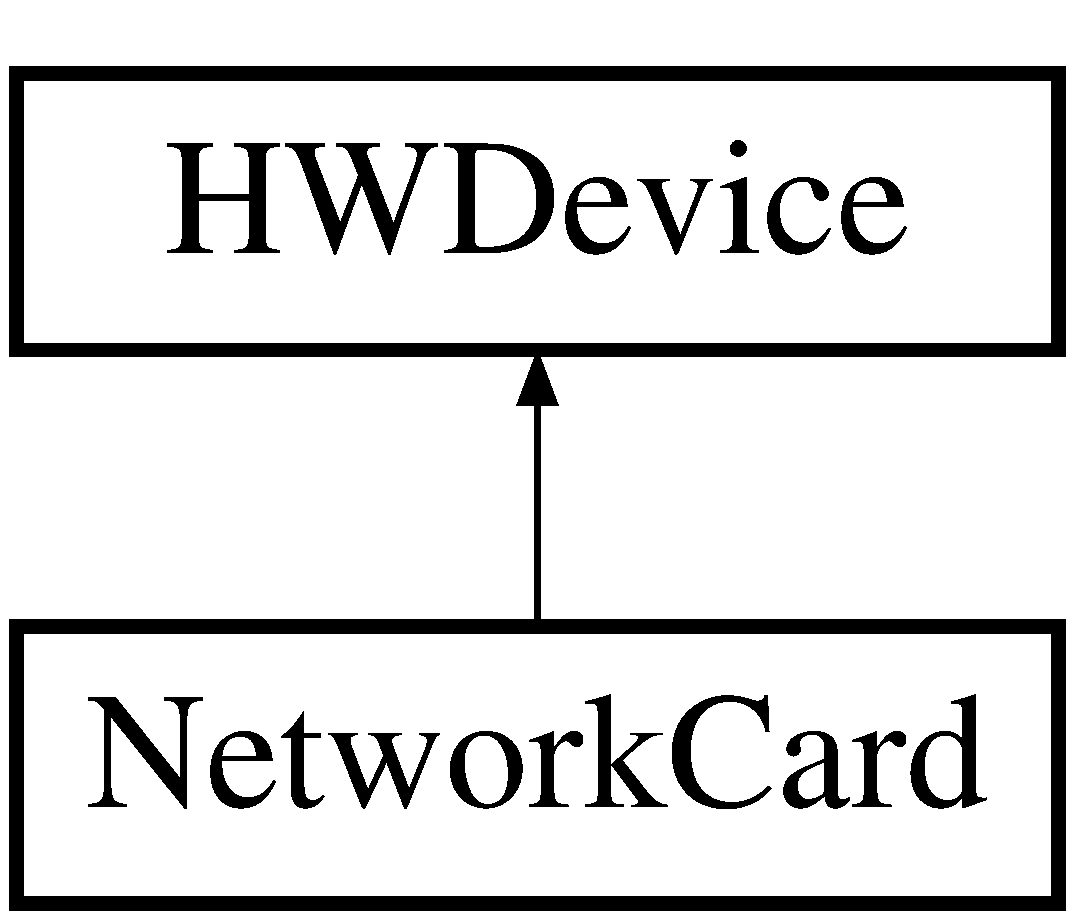
\includegraphics[height=2.000000cm]{classNetworkCard}
\end{center}
\end{figure}
\subsection*{Public Member Functions}
\begin{DoxyCompactItemize}
\item 
{\bfseries Network\+Card} (int position)\hypertarget{classNetworkCard_a6a74d2a0de1390de3ada44a5ee63020f}{}\label{classNetworkCard_a6a74d2a0de1390de3ada44a5ee63020f}

\end{DoxyCompactItemize}
\subsection*{Additional Inherited Members}


\subsection{Detailed Description}
This class represents a generic Network Card 

The documentation for this class was generated from the following file\+:\begin{DoxyCompactItemize}
\item 
/home/doomdiskday/workspace2/main/src/model/\+H\+W/\+Network\+Card/Network\+Card.\+h\end{DoxyCompactItemize}

\hypertarget{classNetworkCardManager}{}\section{Network\+Card\+Manager Class Reference}
\label{classNetworkCardManager}\index{Network\+Card\+Manager@{Network\+Card\+Manager}}


{\ttfamily \#include $<$Network\+Card\+Manager.\+h$>$}

Inheritance diagram for Network\+Card\+Manager\+:\begin{figure}[H]
\begin{center}
\leavevmode
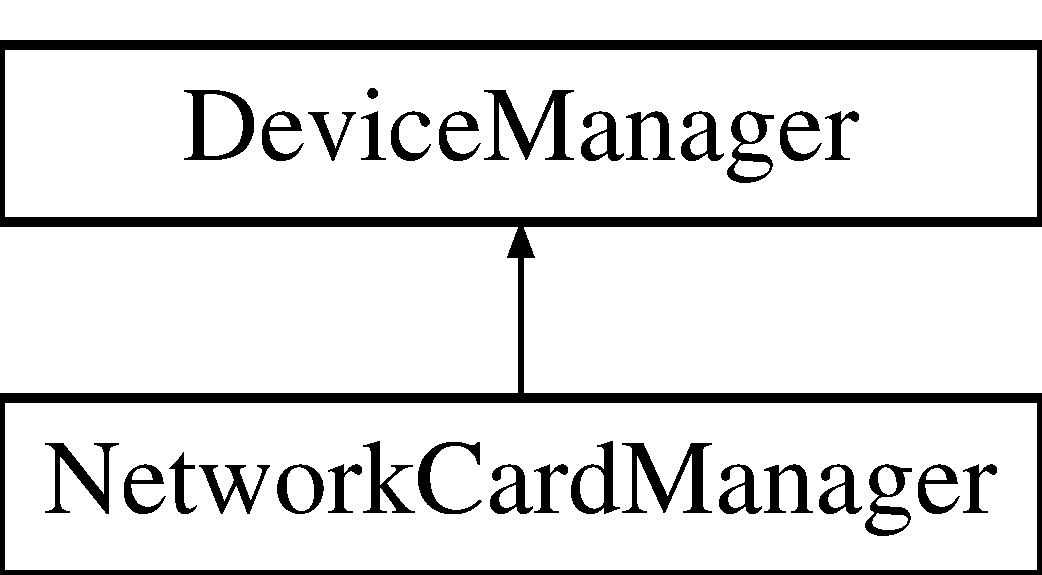
\includegraphics[height=2.000000cm]{classNetworkCardManager}
\end{center}
\end{figure}
\subsection*{Public Member Functions}
\begin{DoxyCompactItemize}
\item 
void \hyperlink{classNetworkCardManager_aa6a77a00f2366720ef0a4cbbe5c01a1d}{generate\+All\+Devices} ()
\item 
\hyperlink{classHWDevice}{H\+W\+Device} $\ast$ \hyperlink{classNetworkCardManager_a675dcf10689da520c3ab5ff32d066811}{generate\+New\+Device} (int position)
\item 
void \hyperlink{classNetworkCardManager_a9204cc788a83cafc73b2f798963417a2}{set\+Commands} (int device\+Position)
\item 
void \hyperlink{classNetworkCardManager_a880800c63daa416ec642691c0d85ca4a}{set\+All\+Infos} (int position)
\item 
\hyperlink{classBaseDifference}{Base\+Difference} $\ast$$\ast$ \hyperlink{classNetworkCardManager_a8dc8b4267433e57c6450fb7ebb0a43f6}{generate\+Log\+Difference} ()
\item 
\hyperlink{classHWDevice}{H\+W\+Device} $\ast$ \hyperlink{classNetworkCardManager_a473a9578d17f85f125183a6c48f86eb8}{generate\+Fake\+Device} ()
\end{DoxyCompactItemize}
\subsection*{Additional Inherited Members}


\subsection{Detailed Description}
Reppresents a Network card manager, it\textquotesingle{}s used to manage all network cards on the system. 

\subsection{Member Function Documentation}
\index{Network\+Card\+Manager@{Network\+Card\+Manager}!generate\+All\+Devices@{generate\+All\+Devices}}
\index{generate\+All\+Devices@{generate\+All\+Devices}!Network\+Card\+Manager@{Network\+Card\+Manager}}
\subsubsection[{\texorpdfstring{generate\+All\+Devices()}{generateAllDevices()}}]{\setlength{\rightskip}{0pt plus 5cm}void Network\+Card\+Manager\+::generate\+All\+Devices (
\begin{DoxyParamCaption}
{}
\end{DoxyParamCaption}
)\hspace{0.3cm}{\ttfamily [virtual]}}\hypertarget{classNetworkCardManager_aa6a77a00f2366720ef0a4cbbe5c01a1d}{}\label{classNetworkCardManager_aa6a77a00f2366720ef0a4cbbe5c01a1d}
Generate and populate the devices array. This method will be overwritten from the specific classes (\hyperlink{classBIOS}{B\+I\+OS}, H\+DD, ecc..) 

Implements \hyperlink{classDeviceManager_ae9fa3bd3aa66f373d7748628b7ba26cc}{Device\+Manager}.

\index{Network\+Card\+Manager@{Network\+Card\+Manager}!generate\+Fake\+Device@{generate\+Fake\+Device}}
\index{generate\+Fake\+Device@{generate\+Fake\+Device}!Network\+Card\+Manager@{Network\+Card\+Manager}}
\subsubsection[{\texorpdfstring{generate\+Fake\+Device()}{generateFakeDevice()}}]{\setlength{\rightskip}{0pt plus 5cm}{\bf H\+W\+Device} $\ast$ Network\+Card\+Manager\+::generate\+Fake\+Device (
\begin{DoxyParamCaption}
{}
\end{DoxyParamCaption}
)\hspace{0.3cm}{\ttfamily [virtual]}}\hypertarget{classNetworkCardManager_a473a9578d17f85f125183a6c48f86eb8}{}\label{classNetworkCardManager_a473a9578d17f85f125183a6c48f86eb8}
This abstract method will produce a Fake (Specified by the concrete classes) Device that will be used later to compare devices 

Implements \hyperlink{classDeviceManager_a218031345b7b61c79f427985d950c3f3}{Device\+Manager}.

\index{Network\+Card\+Manager@{Network\+Card\+Manager}!generate\+Log\+Difference@{generate\+Log\+Difference}}
\index{generate\+Log\+Difference@{generate\+Log\+Difference}!Network\+Card\+Manager@{Network\+Card\+Manager}}
\subsubsection[{\texorpdfstring{generate\+Log\+Difference()}{generateLogDifference()}}]{\setlength{\rightskip}{0pt plus 5cm}{\bf Base\+Difference} $\ast$$\ast$ Network\+Card\+Manager\+::generate\+Log\+Difference (
\begin{DoxyParamCaption}
{}
\end{DoxyParamCaption}
)\hspace{0.3cm}{\ttfamily [virtual]}}\hypertarget{classNetworkCardManager_a8dc8b4267433e57c6450fb7ebb0a43f6}{}\label{classNetworkCardManager_a8dc8b4267433e57c6450fb7ebb0a43f6}
This abstract method will produce a \hyperlink{classBaseDifference}{Base\+Difference}, it will be used to compare different  between them.

\begin{DoxyReturn}{Returns}
the differences to populate 
\end{DoxyReturn}


Implements \hyperlink{classDeviceManager_ae9916011e50a6a48aea3d87b6c44b27e}{Device\+Manager}.

\index{Network\+Card\+Manager@{Network\+Card\+Manager}!generate\+New\+Device@{generate\+New\+Device}}
\index{generate\+New\+Device@{generate\+New\+Device}!Network\+Card\+Manager@{Network\+Card\+Manager}}
\subsubsection[{\texorpdfstring{generate\+New\+Device(int position)}{generateNewDevice(int position)}}]{\setlength{\rightskip}{0pt plus 5cm}{\bf H\+W\+Device} $\ast$ Network\+Card\+Manager\+::generate\+New\+Device (
\begin{DoxyParamCaption}
\item[{int}]{position}
\end{DoxyParamCaption}
)\hspace{0.3cm}{\ttfamily [virtual]}}\hypertarget{classNetworkCardManager_a675dcf10689da520c3ab5ff32d066811}{}\label{classNetworkCardManager_a675dcf10689da520c3ab5ff32d066811}
Generate and return a new device in a specific position.


\begin{DoxyParams}{Parameters}
{\em position} & used by the device \\
\hline
\end{DoxyParams}
\begin{DoxyReturn}{Returns}
the generated device 
\end{DoxyReturn}


Implements \hyperlink{classDeviceManager_a64c7c17d8cb8d407361dbcf8f6f17ccf}{Device\+Manager}.

\index{Network\+Card\+Manager@{Network\+Card\+Manager}!set\+All\+Infos@{set\+All\+Infos}}
\index{set\+All\+Infos@{set\+All\+Infos}!Network\+Card\+Manager@{Network\+Card\+Manager}}
\subsubsection[{\texorpdfstring{set\+All\+Infos(int position)}{setAllInfos(int position)}}]{\setlength{\rightskip}{0pt plus 5cm}void Network\+Card\+Manager\+::set\+All\+Infos (
\begin{DoxyParamCaption}
\item[{int}]{position}
\end{DoxyParamCaption}
)\hspace{0.3cm}{\ttfamily [virtual]}}\hypertarget{classNetworkCardManager_a880800c63daa416ec642691c0d85ca4a}{}\label{classNetworkCardManager_a880800c63daa416ec642691c0d85ca4a}
Set all devices informations, by default this method set all properties using the commands array and pass it, with a visitor, to the property


\begin{DoxyParams}{Parameters}
{\em position} & the device position in the device array \\
\hline
\end{DoxyParams}


Reimplemented from \hyperlink{classDeviceManager_a4c34a8b9035b29829739c533b611ab07}{Device\+Manager}.

\index{Network\+Card\+Manager@{Network\+Card\+Manager}!set\+Commands@{set\+Commands}}
\index{set\+Commands@{set\+Commands}!Network\+Card\+Manager@{Network\+Card\+Manager}}
\subsubsection[{\texorpdfstring{set\+Commands(int device\+Position)}{setCommands(int devicePosition)}}]{\setlength{\rightskip}{0pt plus 5cm}void Network\+Card\+Manager\+::set\+Commands (
\begin{DoxyParamCaption}
\item[{int}]{device\+Position}
\end{DoxyParamCaption}
)\hspace{0.3cm}{\ttfamily [virtual]}}\hypertarget{classNetworkCardManager_a9204cc788a83cafc73b2f798963417a2}{}\label{classNetworkCardManager_a9204cc788a83cafc73b2f798963417a2}
Set all commands used to retrieve infos. This method will be overwritten from the specific classes (\hyperlink{classBIOS}{B\+I\+OS}, H\+DD, ecc...)


\begin{DoxyParams}{Parameters}
{\em device\+Position} & the device position in the devices array \\
\hline
\end{DoxyParams}


Implements \hyperlink{classDeviceManager_ae367c6847b2988cf6249cbf6254261cb}{Device\+Manager}.



The documentation for this class was generated from the following files\+:\begin{DoxyCompactItemize}
\item 
/home/doomdiskday/workspace2/main/src/model/\+H\+W/\+Network\+Card/Network\+Card\+Manager.\+h\item 
/home/doomdiskday/workspace2/main/src/model/\+H\+W/\+Network\+Card/Network\+Card\+Manager.\+cpp\end{DoxyCompactItemize}

\hypertarget{classStringManager}{}\section{String\+Manager Class Reference}
\label{classStringManager}\index{String\+Manager@{String\+Manager}}
\subsection*{Public Member Functions}
\begin{DoxyCompactItemize}
\item 
string \hyperlink{classStringManager_a5b7c33e4a32695316cf1f3135409ae2e}{get\+Sub\+String} (string to\+Filter, string filter, bool before\+The\+Filter)
\item 
string \hyperlink{classStringManager_a536560162badf4e7436c885b8d72871c}{get\+Property} (string to\+Filter, string property)
\item 
string \hyperlink{classStringManager_ad44b7aa8859dde0fe235efeab3d5c0b7}{trimmed} (std\+::string s)
\item 
bool \hyperlink{classStringManager_a04d29318d90a6d342a0b504d4bcba389}{is\+Number} (string to\+Check)
\end{DoxyCompactItemize}


\subsection{Member Function Documentation}
\index{String\+Manager@{String\+Manager}!get\+Property@{get\+Property}}
\index{get\+Property@{get\+Property}!String\+Manager@{String\+Manager}}
\subsubsection[{\texorpdfstring{get\+Property(string to\+Filter, string property)}{getProperty(string toFilter, string property)}}]{\setlength{\rightskip}{0pt plus 5cm}string String\+Manager\+::get\+Property (
\begin{DoxyParamCaption}
\item[{string}]{to\+Filter, }
\item[{string}]{property}
\end{DoxyParamCaption}
)}\hypertarget{classStringManager_a536560162badf4e7436c885b8d72871c}{}\label{classStringManager_a536560162badf4e7436c885b8d72871c}
return a filtered(filter= \char`\"{}\+:\char`\"{}) property


\begin{DoxyParams}{Parameters}
{\em to\+Filter} & the string to filter to extrapolate the property \\
\hline
{\em property} & the property to filter \\
\hline
\end{DoxyParams}
\begin{DoxyReturn}{Returns}
the filtered property 
\end{DoxyReturn}
\index{String\+Manager@{String\+Manager}!get\+Sub\+String@{get\+Sub\+String}}
\index{get\+Sub\+String@{get\+Sub\+String}!String\+Manager@{String\+Manager}}
\subsubsection[{\texorpdfstring{get\+Sub\+String(string to\+Filter, string filter, bool before\+The\+Filter)}{getSubString(string toFilter, string filter, bool beforeTheFilter)}}]{\setlength{\rightskip}{0pt plus 5cm}string String\+Manager\+::get\+Sub\+String (
\begin{DoxyParamCaption}
\item[{string}]{to\+Filter, }
\item[{string}]{filter, }
\item[{bool}]{before\+The\+Filter}
\end{DoxyParamCaption}
)}\hypertarget{classStringManager_a5b7c33e4a32695316cf1f3135409ae2e}{}\label{classStringManager_a5b7c33e4a32695316cf1f3135409ae2e}
return a filtered string


\begin{DoxyParams}{Parameters}
{\em to\+Filter} & string to filter \\
\hline
{\em filter} & filter to use \\
\hline
{\em before\+The\+Filter} & (T\+R\+UE=Filter before the string, F\+A\+L\+SE=Filter after the string) \\
\hline
\end{DoxyParams}
\index{String\+Manager@{String\+Manager}!is\+Number@{is\+Number}}
\index{is\+Number@{is\+Number}!String\+Manager@{String\+Manager}}
\subsubsection[{\texorpdfstring{is\+Number(string to\+Check)}{isNumber(string toCheck)}}]{\setlength{\rightskip}{0pt plus 5cm}bool String\+Manager\+::is\+Number (
\begin{DoxyParamCaption}
\item[{string}]{to\+Check}
\end{DoxyParamCaption}
)}\hypertarget{classStringManager_a04d29318d90a6d342a0b504d4bcba389}{}\label{classStringManager_a04d29318d90a6d342a0b504d4bcba389}
Check if a string passed is a number or not \index{String\+Manager@{String\+Manager}!trimmed@{trimmed}}
\index{trimmed@{trimmed}!String\+Manager@{String\+Manager}}
\subsubsection[{\texorpdfstring{trimmed(std\+::string s)}{trimmed(std::string s)}}]{\setlength{\rightskip}{0pt plus 5cm}std\+::string String\+Manager\+::trimmed (
\begin{DoxyParamCaption}
\item[{std\+::string}]{s}
\end{DoxyParamCaption}
)}\hypertarget{classStringManager_ad44b7aa8859dde0fe235efeab3d5c0b7}{}\label{classStringManager_ad44b7aa8859dde0fe235efeab3d5c0b7}
Trim a string


\begin{DoxyParams}{Parameters}
{\em s} & string to trim \\
\hline
\end{DoxyParams}
\begin{DoxyReturn}{Returns}
trimmed string 
\end{DoxyReturn}


The documentation for this class was generated from the following files\+:\begin{DoxyCompactItemize}
\item 
/home/doomdiskday/workspace2/main/src/utils/String\+Manager.\+h\item 
/home/doomdiskday/workspace2/main/src/utils/String\+Manager.\+cpp\end{DoxyCompactItemize}

\hypertarget{classVisitor}{}\section{Visitor Class Reference}
\label{classVisitor}\index{Visitor@{Visitor}}


{\ttfamily \#include $<$Visitor.\+h$>$}

Inheritance diagram for Visitor\+:\begin{figure}[H]
\begin{center}
\leavevmode
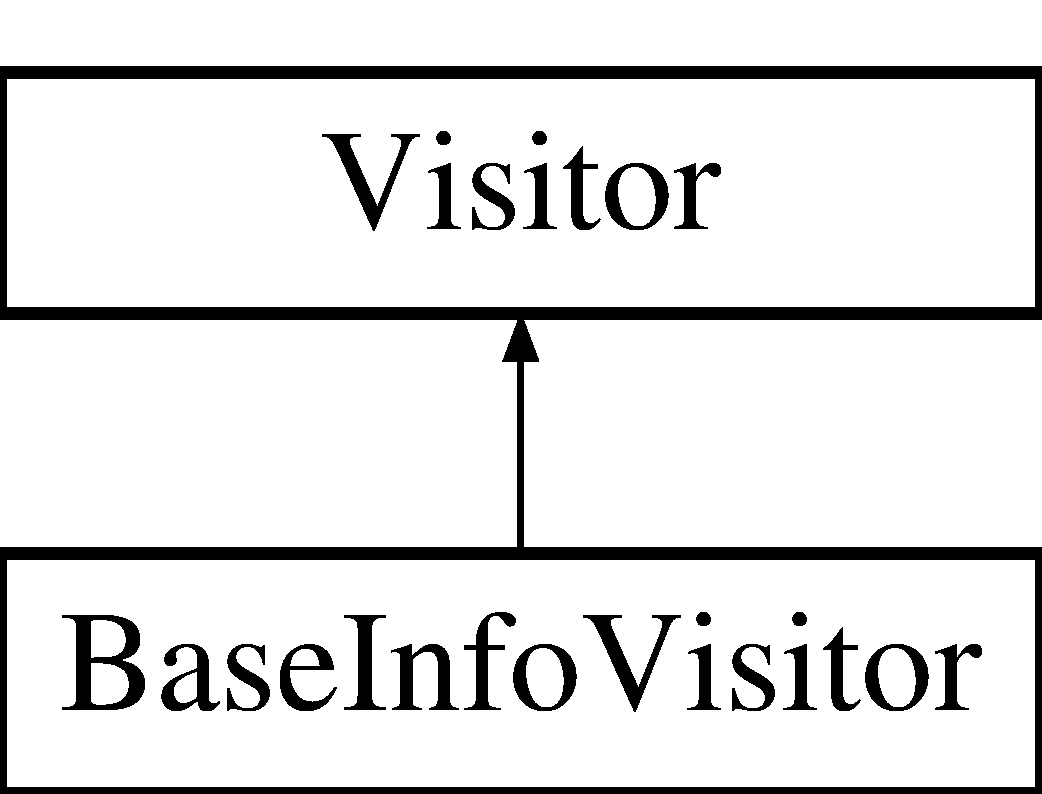
\includegraphics[height=2.000000cm]{classVisitor}
\end{center}
\end{figure}
\subsection*{Public Member Functions}
\begin{DoxyCompactItemize}
\item 
virtual void \hyperlink{classVisitor_aa290c4e12905eb700f631b83ce77deea}{visit\+Base\+Info\+With\+Command} (int \&v, \hyperlink{classCommand}{Command} $\ast$cmd)=0
\item 
virtual void \hyperlink{classVisitor_aa6045f028cc91712ab5cca38e1461d39}{visit\+Base\+Info\+With\+Command} (string \&v, \hyperlink{classCommand}{Command} $\ast$cmd)=0
\item 
virtual void \hyperlink{classVisitor_a3d6f39af42e955dcd56d1d928f6edfe2}{visit\+Base\+Info\+To\+Print} (int v, string property)=0
\item 
virtual void \hyperlink{classVisitor_a9f87fbabd6b8cd4d5456d81faff2c31a}{visit\+Base\+Info\+To\+Print} (string v, string property)=0
\item 
virtual void \hyperlink{classVisitor_addcf4dbedba4a2ba739d0fdef144eb6d}{visit\+Base\+Info\+To\+Log} (int v, string property, F\+I\+LE $\ast$log\+File)=0
\item 
virtual void \hyperlink{classVisitor_a591ed3a6edd9b31a8a1b2847c5a22e29}{visit\+Base\+Info\+To\+Log} (string v, string property, F\+I\+LE $\ast$log\+File)=0
\item 
virtual void \hyperlink{classVisitor_a766dd43ac0c15f92b15a5b0fb90deca9}{visit\+Base\+Info\+With\+Value} (int \&v, string to\+Assign)=0
\item 
virtual void \hyperlink{classVisitor_afb85cf66df37046633ef80f085c8c4fe}{visit\+Base\+Info\+With\+Value} (string \&v, string to\+Assign)=0
\item 
virtual void \hyperlink{classVisitor_a3e8e80f88fd9513a971f4db4cde00ef7}{visit\+Log\+To\+Print} (bool check, string prop, string value)=0
\item 
virtual void \hyperlink{classVisitor_ac889258497b1a2c2d673de0ceb3b227b}{visit\+Log\+To\+Print} (bool check, string prop, int value)=0
\end{DoxyCompactItemize}


\subsection{Detailed Description}
This class rappresents a generic visitor. It\textquotesingle{}s used to visit and manage (set, print, log) both property and logdifferences. 

\subsection{Member Function Documentation}
\index{Visitor@{Visitor}!visit\+Base\+Info\+To\+Log@{visit\+Base\+Info\+To\+Log}}
\index{visit\+Base\+Info\+To\+Log@{visit\+Base\+Info\+To\+Log}!Visitor@{Visitor}}
\subsubsection[{\texorpdfstring{visit\+Base\+Info\+To\+Log(int v, string property, F\+I\+L\+E $\ast$log\+File)=0}{visitBaseInfoToLog(int v, string property, FILE *logFile)=0}}]{\setlength{\rightskip}{0pt plus 5cm}virtual void Visitor\+::visit\+Base\+Info\+To\+Log (
\begin{DoxyParamCaption}
\item[{int}]{v, }
\item[{string}]{property, }
\item[{F\+I\+LE $\ast$}]{log\+File}
\end{DoxyParamCaption}
)\hspace{0.3cm}{\ttfamily [pure virtual]}}\hypertarget{classVisitor_addcf4dbedba4a2ba739d0fdef144eb6d}{}\label{classVisitor_addcf4dbedba4a2ba739d0fdef144eb6d}
Method used to visit a baseinfo and log his value and his property


\begin{DoxyParams}{Parameters}
{\em v} & the int value to log \\
\hline
{\em property} & the property to log \\
\hline
{\em log\+File} & the log file to populate. \\
\hline
\end{DoxyParams}


Implemented in \hyperlink{classBaseInfoVisitor_adf0f9a3ad34d26595ee2cb78cc370a65}{Base\+Info\+Visitor}.

\index{Visitor@{Visitor}!visit\+Base\+Info\+To\+Log@{visit\+Base\+Info\+To\+Log}}
\index{visit\+Base\+Info\+To\+Log@{visit\+Base\+Info\+To\+Log}!Visitor@{Visitor}}
\subsubsection[{\texorpdfstring{visit\+Base\+Info\+To\+Log(string v, string property, F\+I\+L\+E $\ast$log\+File)=0}{visitBaseInfoToLog(string v, string property, FILE *logFile)=0}}]{\setlength{\rightskip}{0pt plus 5cm}virtual void Visitor\+::visit\+Base\+Info\+To\+Log (
\begin{DoxyParamCaption}
\item[{string}]{v, }
\item[{string}]{property, }
\item[{F\+I\+LE $\ast$}]{log\+File}
\end{DoxyParamCaption}
)\hspace{0.3cm}{\ttfamily [pure virtual]}}\hypertarget{classVisitor_a591ed3a6edd9b31a8a1b2847c5a22e29}{}\label{classVisitor_a591ed3a6edd9b31a8a1b2847c5a22e29}
Method used to visit a baseinfo and log his value and his property


\begin{DoxyParams}{Parameters}
{\em v} & the string value to log \\
\hline
{\em property} & the property to log \\
\hline
{\em log\+File} & the log file to populate. \\
\hline
\end{DoxyParams}


Implemented in \hyperlink{classBaseInfoVisitor_a8590d40b5c1c277dee482518ad31c494}{Base\+Info\+Visitor}.

\index{Visitor@{Visitor}!visit\+Base\+Info\+To\+Print@{visit\+Base\+Info\+To\+Print}}
\index{visit\+Base\+Info\+To\+Print@{visit\+Base\+Info\+To\+Print}!Visitor@{Visitor}}
\subsubsection[{\texorpdfstring{visit\+Base\+Info\+To\+Print(int v, string property)=0}{visitBaseInfoToPrint(int v, string property)=0}}]{\setlength{\rightskip}{0pt plus 5cm}virtual void Visitor\+::visit\+Base\+Info\+To\+Print (
\begin{DoxyParamCaption}
\item[{int}]{v, }
\item[{string}]{property}
\end{DoxyParamCaption}
)\hspace{0.3cm}{\ttfamily [pure virtual]}}\hypertarget{classVisitor_a3d6f39af42e955dcd56d1d928f6edfe2}{}\label{classVisitor_a3d6f39af42e955dcd56d1d928f6edfe2}
Method used to visit a baseinfo and print his value and his property


\begin{DoxyParams}{Parameters}
{\em v} & the int value to print \\
\hline
{\em property} & the property to print \\
\hline
\end{DoxyParams}


Implemented in \hyperlink{classBaseInfoVisitor_a395234ebebdfbaf4f7e155bfc0a5aa5d}{Base\+Info\+Visitor}.

\index{Visitor@{Visitor}!visit\+Base\+Info\+To\+Print@{visit\+Base\+Info\+To\+Print}}
\index{visit\+Base\+Info\+To\+Print@{visit\+Base\+Info\+To\+Print}!Visitor@{Visitor}}
\subsubsection[{\texorpdfstring{visit\+Base\+Info\+To\+Print(string v, string property)=0}{visitBaseInfoToPrint(string v, string property)=0}}]{\setlength{\rightskip}{0pt plus 5cm}virtual void Visitor\+::visit\+Base\+Info\+To\+Print (
\begin{DoxyParamCaption}
\item[{string}]{v, }
\item[{string}]{property}
\end{DoxyParamCaption}
)\hspace{0.3cm}{\ttfamily [pure virtual]}}\hypertarget{classVisitor_a9f87fbabd6b8cd4d5456d81faff2c31a}{}\label{classVisitor_a9f87fbabd6b8cd4d5456d81faff2c31a}
Method used to visit a baseinfo and print his value and his property


\begin{DoxyParams}{Parameters}
{\em v} & the string value to print \\
\hline
{\em property} & the property to print \\
\hline
\end{DoxyParams}


Implemented in \hyperlink{classBaseInfoVisitor_a5be08c690d21e5c1d9257efdf0a75ca4}{Base\+Info\+Visitor}.

\index{Visitor@{Visitor}!visit\+Base\+Info\+With\+Command@{visit\+Base\+Info\+With\+Command}}
\index{visit\+Base\+Info\+With\+Command@{visit\+Base\+Info\+With\+Command}!Visitor@{Visitor}}
\subsubsection[{\texorpdfstring{visit\+Base\+Info\+With\+Command(int \&v, Command $\ast$cmd)=0}{visitBaseInfoWithCommand(int &v, Command *cmd)=0}}]{\setlength{\rightskip}{0pt plus 5cm}virtual void Visitor\+::visit\+Base\+Info\+With\+Command (
\begin{DoxyParamCaption}
\item[{int \&}]{v, }
\item[{{\bf Command} $\ast$}]{cmd}
\end{DoxyParamCaption}
)\hspace{0.3cm}{\ttfamily [pure virtual]}}\hypertarget{classVisitor_aa290c4e12905eb700f631b83ce77deea}{}\label{classVisitor_aa290c4e12905eb700f631b83ce77deea}
Method used to visit a baseinfo and set his value to an information retrieved by a command passed by param


\begin{DoxyParams}{Parameters}
{\em v} & the int value to set \\
\hline
{\em cmd} & the command used \\
\hline
\end{DoxyParams}


Implemented in \hyperlink{classBaseInfoVisitor_a96013581736191e0c186746f061b6d2e}{Base\+Info\+Visitor}.

\index{Visitor@{Visitor}!visit\+Base\+Info\+With\+Command@{visit\+Base\+Info\+With\+Command}}
\index{visit\+Base\+Info\+With\+Command@{visit\+Base\+Info\+With\+Command}!Visitor@{Visitor}}
\subsubsection[{\texorpdfstring{visit\+Base\+Info\+With\+Command(string \&v, Command $\ast$cmd)=0}{visitBaseInfoWithCommand(string &v, Command *cmd)=0}}]{\setlength{\rightskip}{0pt plus 5cm}virtual void Visitor\+::visit\+Base\+Info\+With\+Command (
\begin{DoxyParamCaption}
\item[{string \&}]{v, }
\item[{{\bf Command} $\ast$}]{cmd}
\end{DoxyParamCaption}
)\hspace{0.3cm}{\ttfamily [pure virtual]}}\hypertarget{classVisitor_aa6045f028cc91712ab5cca38e1461d39}{}\label{classVisitor_aa6045f028cc91712ab5cca38e1461d39}
Method used to visit a baseinfo and set his value to an information retrieved by a command passed by param


\begin{DoxyParams}{Parameters}
{\em v} & the string value to set \\
\hline
{\em cmd} & the command used \\
\hline
\end{DoxyParams}


Implemented in \hyperlink{classBaseInfoVisitor_a8615d145a52433f981a147642038fe91}{Base\+Info\+Visitor}.

\index{Visitor@{Visitor}!visit\+Base\+Info\+With\+Value@{visit\+Base\+Info\+With\+Value}}
\index{visit\+Base\+Info\+With\+Value@{visit\+Base\+Info\+With\+Value}!Visitor@{Visitor}}
\subsubsection[{\texorpdfstring{visit\+Base\+Info\+With\+Value(int \&v, string to\+Assign)=0}{visitBaseInfoWithValue(int &v, string toAssign)=0}}]{\setlength{\rightskip}{0pt plus 5cm}virtual void Visitor\+::visit\+Base\+Info\+With\+Value (
\begin{DoxyParamCaption}
\item[{int \&}]{v, }
\item[{string}]{to\+Assign}
\end{DoxyParamCaption}
)\hspace{0.3cm}{\ttfamily [pure virtual]}}\hypertarget{classVisitor_a766dd43ac0c15f92b15a5b0fb90deca9}{}\label{classVisitor_a766dd43ac0c15f92b15a5b0fb90deca9}
Method used to visit a baseinfo and set his value.


\begin{DoxyParams}{Parameters}
{\em v} & the int value to set \\
\hline
{\em property} & the property to set \\
\hline
\end{DoxyParams}


Implemented in \hyperlink{classBaseInfoVisitor_a56c3bb5a441e77566e62881e5a82b9d8}{Base\+Info\+Visitor}.

\index{Visitor@{Visitor}!visit\+Base\+Info\+With\+Value@{visit\+Base\+Info\+With\+Value}}
\index{visit\+Base\+Info\+With\+Value@{visit\+Base\+Info\+With\+Value}!Visitor@{Visitor}}
\subsubsection[{\texorpdfstring{visit\+Base\+Info\+With\+Value(string \&v, string to\+Assign)=0}{visitBaseInfoWithValue(string &v, string toAssign)=0}}]{\setlength{\rightskip}{0pt plus 5cm}virtual void Visitor\+::visit\+Base\+Info\+With\+Value (
\begin{DoxyParamCaption}
\item[{string \&}]{v, }
\item[{string}]{to\+Assign}
\end{DoxyParamCaption}
)\hspace{0.3cm}{\ttfamily [pure virtual]}}\hypertarget{classVisitor_afb85cf66df37046633ef80f085c8c4fe}{}\label{classVisitor_afb85cf66df37046633ef80f085c8c4fe}
Method used to visit a baseinfo and set his value.


\begin{DoxyParams}{Parameters}
{\em v} & the string value to set \\
\hline
{\em property} & the property to set \\
\hline
\end{DoxyParams}


Implemented in \hyperlink{classBaseInfoVisitor_adc07ce4d4919fccad038d90c9c820178}{Base\+Info\+Visitor}.

\index{Visitor@{Visitor}!visit\+Log\+To\+Print@{visit\+Log\+To\+Print}}
\index{visit\+Log\+To\+Print@{visit\+Log\+To\+Print}!Visitor@{Visitor}}
\subsubsection[{\texorpdfstring{visit\+Log\+To\+Print(bool check, string prop, string value)=0}{visitLogToPrint(bool check, string prop, string value)=0}}]{\setlength{\rightskip}{0pt plus 5cm}virtual void Visitor\+::visit\+Log\+To\+Print (
\begin{DoxyParamCaption}
\item[{bool}]{check, }
\item[{string}]{prop, }
\item[{string}]{value}
\end{DoxyParamCaption}
)\hspace{0.3cm}{\ttfamily [pure virtual]}}\hypertarget{classVisitor_a3e8e80f88fd9513a971f4db4cde00ef7}{}\label{classVisitor_a3e8e80f88fd9513a971f4db4cde00ef7}
Method used to visit a log file and populate it


\begin{DoxyParams}{Parameters}
{\em check} & the check value \\
\hline
{\em prop} & the property checked \\
\hline
{\em value} & the value checked \\
\hline
\end{DoxyParams}


Implemented in \hyperlink{classBaseInfoVisitor_ad0c9667e9004fd1494f79b09947b0620}{Base\+Info\+Visitor}.

\index{Visitor@{Visitor}!visit\+Log\+To\+Print@{visit\+Log\+To\+Print}}
\index{visit\+Log\+To\+Print@{visit\+Log\+To\+Print}!Visitor@{Visitor}}
\subsubsection[{\texorpdfstring{visit\+Log\+To\+Print(bool check, string prop, int value)=0}{visitLogToPrint(bool check, string prop, int value)=0}}]{\setlength{\rightskip}{0pt plus 5cm}virtual void Visitor\+::visit\+Log\+To\+Print (
\begin{DoxyParamCaption}
\item[{bool}]{check, }
\item[{string}]{prop, }
\item[{int}]{value}
\end{DoxyParamCaption}
)\hspace{0.3cm}{\ttfamily [pure virtual]}}\hypertarget{classVisitor_ac889258497b1a2c2d673de0ceb3b227b}{}\label{classVisitor_ac889258497b1a2c2d673de0ceb3b227b}
Method used to visit a log file and populate it


\begin{DoxyParams}{Parameters}
{\em check} & the check value \\
\hline
{\em prop} & the property checked \\
\hline
{\em value} & the value checked \\
\hline
\end{DoxyParams}


Implemented in \hyperlink{classBaseInfoVisitor_a326f9be710640548f76a08253422318a}{Base\+Info\+Visitor}.



The documentation for this class was generated from the following file\+:\begin{DoxyCompactItemize}
\item 
/home/doomdiskday/workspace2/main/src/model/\+H\+W/\+Visitors/Visitor.\+h\end{DoxyCompactItemize}

%--- End generated contents ---

% Index
\backmatter
\newpage
\phantomsection
\clearemptydoublepage
\addcontentsline{toc}{chapter}{Index}
\printindex

\end{document}
